\chapter{Réalisation}
	
\section*{Introduction}
\addcontentsline{toc}{section}{Introduction }
    Le quatrième chapitre sera consacré à la mise en œuvre concrète du projet.
     Nous explorerons les choix techniques que nous avons adoptés et détaillerons le travail effectué pour donner vie à notre solution.

\section{Choix technologiques}
\par  Dans cette partie, nous explorerons les décisions stratégiques que nous avons pris concernant les technologies et les outils choisises pour la réalisation de notre solution.     
\subsection{Frameworks et base de données}
    \begin{itemize}
        \item\textbf{FastAPI : }
            \par FastAPI est un framework web moderne et rapide (à haute performance) pour la création d'API avec Python,
            basé sur les annotations de type standard de Python\cite{fastapi}. 
            \par Dans la réalisation de ce projet, nous avons opté pour le choix de FastApi comme notre backend framework vue ces performances extrêmement élevées, comparables à celles de NodeJS et Go, grâce à l'utilisation de Starlette et Pydantic.
            FastAPI est l'un des frameworks Python les plus rapides.
            \par Sa Robustesse aussi, car il permet de produire un code prêt pour la production avec une documentation interactive et automatique.
        \item\textbf{ReactJS : }
                    \par React est une bibliothèque JavaScript destinée à la création d'interfaces utilisateur (UI) \cite{react}. 
                    \par Dans la réalisation de ce projet, nous avons opté pour React comme étant notre frontend framework car il 
                    permet de créer des interfaces utilisateur dynamiques et réactives avec une efficacité accrue grâce à sa gestion 
                    intelligente des mises à jour via le DOM virtuel.
        \item\textbf{PostgreSQL : }
                    \par PostgreSQL est un puissant système de gestion base de données relationnelle (SGBD) objet open source, développé activement depuis plus 
                    de 35 ans, qui lui a valu une solide réputation en termes de fiabilité, de robustesse des fonctionnalités et de performances\cite{pg}. 
                    \par Dans la réalisation de ce projet, nous avons opté pour le choix de PostgreSQL comme étant notre SGBD vue qu'il est souvent perçu comme un 
                    système plus fiable et plus robuste que MySQL pour gérer de grands volumes de données sans risque de corruption.
                    \par De plus, il permet de stocker des informations de manière plus structurée grâce à une meilleure gestion des relations et
                     des contraintes.
                \end{itemize}

\subsection{Outils de communication}
\begin{itemize}
    \item\textbf{MQTT : }
                \par Message Queuing Telemetry Transport (MQTT) est un protocole de messagerie basé sur des normes, ou un ensemble de règles, utilisé pour la communication de machine à machine \cite{mqtt}. 
                \par Dans la réalisation de ce projet, nous avons opté pour MQTT comme étant un systéme de notification car il facilite le chiffrement des messages 
                via TLS et l'authentification des clients à l'aide de protocoles d'authentification modernes, tels que OAuth. 
                \par De plus, sa Légèreté et efficacité car les clients MQTT sont très petits, ils nécessitent peu de ressources. 
                Les en-têtes des messages MQTT sont de petite taille afin d'optimiser la bande passante du réseau.

    \item\textbf{RESTful APIs :}
    
            \par REpresentational State Transfer (REST) constitue un style architectural et un mode de communication fréquemment utilisé dans le développement de services Web \cite{rest}. 
            \par Dans la réalisation de ce projet, nous avons opté pour RESTful API comme étant le mode de communiction entre les différents microservices du systéme car ils sont faciles à utiliser avec la plupart des outils. 
            \par De plus REST s'impose progressivement comme le standard pour l'interaction entre systèmes. 

    \end{itemize}
\subsection{Bibliothèques pour l'analyse et la manipulation des données}
    \begin{itemize}
        \item\textbf{snowflake.connector : }
                 \par Le connecteur Snowflake pour Python fournit une interface pour le développement d'applications Python
                  qui peuvent se connecter à Snowflake et effectuer toutes les opérations standard.\cite{sncn}. 
                 \par Il a été conçu pour gérer les ressources principales de Snowflake, y compris les bases de données, les schémas, les tables, les tâches et les entrepôts, sans utiliser le langage SQL.
        \item\textbf{psycopg : }
                \par Psycopg est l'adaptateur de base de données PostgreSQL le plus populaire pour le langage de programmation Python. 
                Il est écrit en C et fournit un moyen d'effectuer toute la gamme des opérations SQL sur les bases de données PostgreSQL\cite{psycopg}. 
                \par Il a été conçu pour les applications fortement multithreadées qui créent et détruisent de nombreux curseurs et effectuent un grand nombre d'<<INSERT>>s ou d' <<UPDATE>>s simultanés. C'est le principal raison pour lequel nous avons choisi cet librairie pour toute interaction avec postgresql.
        \item\textbf{Pandas : }
                    \par  Pandas est une bibliothèque de manipulation de données Python qui fournit des structures de données flexibles pour l'analyse des données\cite{pandas}. 
                    \par Il a été conçu pour faciliter l'importation, la manipulation et l'analyse des données, ce qui en fait un choix idéal pour notre projet.
        \item \textbf{GMQTT : }
            \par GMQTT est une bibliothèque de broker MQTT flexible et performante qui implémente entièrement le protocole MQTT V3.x et V5 en golang \cite{gmqtt}. 
   \end{itemize}
\subsection{Bibliothèques d'interaction avec le système d'exploitation}
\begin{itemize}
    \item\textbf{OS : }
        \par Un module intégré à Python qui permet d'interagir avec le système d'exploitation sous-jacent sur lequel Python est exécuté. 
        Il peut être utilisé pour manipuler le système de fichiers, gérer les variables d'environnement, contrôler les processus, et bien plus encore\cite{os}.

    \item \textbf{Scheduler : }
        \par C'est une bibliothèque d'ordonnancement en python avec asyncio, threading ainsi que la prise en charge des fuseaux horaires.
         Elle permet de planifier des tâches en fonction de leurs cycles temporels, d'heures fixes, de jours de la semaine,
         de dates, de poids, de décalages et de comptes d'exécution, et automatiser les tâches\cite{scheduler}.
    \item \textbf{Requests : }
        \par c'est un standard Python permettant d'effectuer des requêtes HTTP.
         Elle cache les subtilités des requêtes derrière une API simple, ce qui permet de concentrer sur l'interaction avec les services et la consommation de données dans l'application\cite{requests}.
    
\end{itemize}
\subsection{Outils de test}
\begin{itemize}
    \item \textbf{Postman : }
                \par  Postman agit en tant que client et constitue un excellent outil pour tester des API RESTful. Il offre une interface utilisateur élégante pour effectuer des requêtes HTTP,
                 sans avoir à écrire beaucoup de code uniquement pour tester les fonctionnalités d'une API. 
                 Postman permet également d'analyser les réponses et de visualiser clairement les en-têtes, le corps et le statut HTTP \cite{postman}. 
    \item\textbf{MQTTX :}
            \par MQTTX est un client de bureau MQTT 5.0 open-source et multiplateforme initialement développé par EMQ, qui peut fonctionner sur n'importe quel systéme d'exploitation.
            \par il rend le développement et le test d'applications MQTT plus rapides et plus faciles\cite{mqttx}.
    \end{itemize}
    \subsection{Outils de versionning}
    \begin{itemize}
        \item \textbf{Git : }
                    \par Git est, de loin, le système de contrôle de version le plus largement utilisé aujourd'hui. C'est un projet open source avancé, activement maintenu. 
                     Grâce à sa structure décentralisée, Git illustre parfaitement ce qu'est un système de contrôle de version décentralisé (DVCS)\cite{git}.
        \item\textbf{Github :}
                \par GitHub est un service d'hébergement Open-Source, permettant aux programmeurs et aux développeurs de partager le code informatique de leurs projets afin de travailler dessus de façon collaborative. On peut le considérer comme un Cloud dédié au code informatique\cite{github}.
        \end{itemize}
    \subsection{Outils de documentation}
        \begin{itemize}
            \item\textbf{Swagger : }
                        \par Swagger est un outil spécialisé qui génère automatiquement la documentation des API RESTful des application.  
                        Son principal avantage réside dans la possibilité de consulter tous les points de terminaison de l'application et de les tester immédiatement en envoyant des requêtes et en recevant des réponses\cite{swagger}.
            \item\textbf{Latex :}

                    \par LaTeX est à la fois un langage de balisage et un logiciel de composition de documents,
                     largement utilisé par la communauté scientifique.
                      il facilite la rédaction de documents volumineux comme les mémoires et les thèses\cite{latex}.
            \item\textbf{Draw.io:}
                    \par Draw.io est une application en ligne gratuite, accessible via un navigateur web, permettant de dessiner des diagrammes et des organigrammes. 
                    Cet outil offre la possibilité de concevoir toutes sortes de diagrammes et de dessins vectoriels, de les enregistrer au format XML, puis de les exporter \cite{draw}.
            \end{itemize}
\section{Réalisation}
\par Dans cette section, nous allons présenter la réalisation de ce projet en illustrant chaque partie avec des captures explicatifs.
\subsection{Micro-service << ETL\_Service >>}
\par Le micro-service ETL\_Service est responsable de l'extraction, de la transformation et du chargement des données de Snowflake vers la base de données PostgreSQL de cette application.
\par Ce micro-service représente une tâche planifiée (cron job), il est programmée de s'éxécuter quotidiennement (chaque 12 ou 24 heurs par exemple) pour mettre à jours les données à monitorer. 
% % \par La figure \textbf{\ref{fig:etl}} représente le resultat de l'api déclancheur de ce micro-service :
% % \begin{figure}[H]
% %     \centering
% %     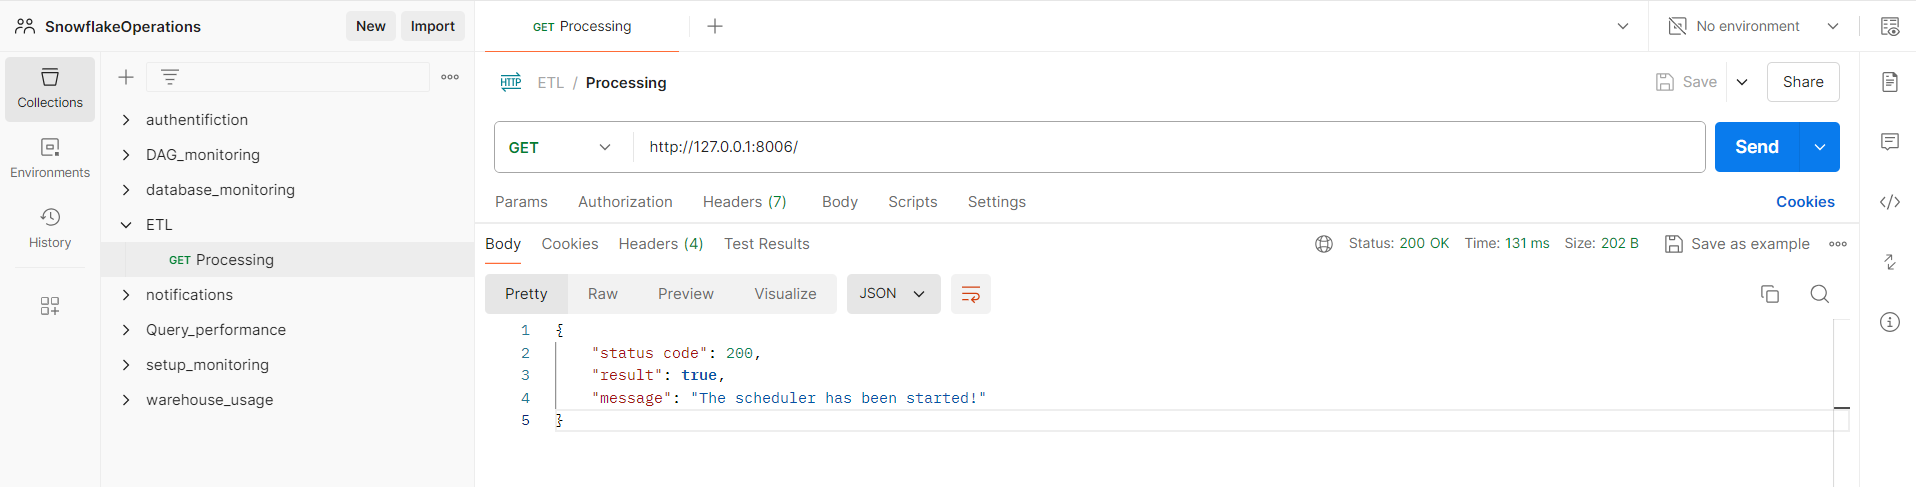
\includegraphics[width =1\linewidth]{img/captures/etl/api.PNG}
% %     \caption{API déclancheur du microservice <<Athentification\_service>> }
% %         \label{fig:etl}
% % \end{figure}
% \par ce micro-service représente une tâche planifiée(cron job) à son tour déclanche le plannificateur de l'exécution en arriére plan comme l'indique la figure \textbf{\ref{fig:launcher}} suivante :
% \begin{figure}[H]
%     \centering
%     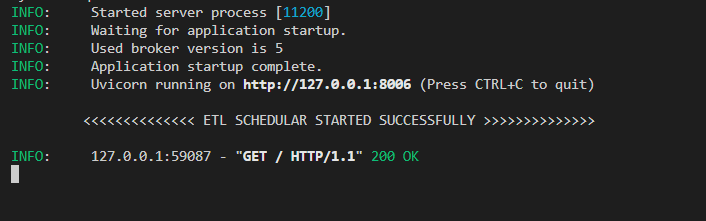
\includegraphics[width =1\linewidth]{img/captures/etl/launcher.PNG}
%     \caption{Déclanchement du plannificateur ETL}
%         \label{fig:launcher}
% \end{figure}
\par Dans le cas où la plannification est atteinte, l'exécution du process ETL se commence par l'archivage des anciennes données pour garantir la disponibilité de la platforme en cas d'échéance de la base de données principale.  
Ensuite, il va extraire les nouvelles données de chaque table systéme de Snowflake en faisant le nettoyage et la transformation sur ces derniers. 
\par  La figure \textbf{\ref{fig:result}} illustre les affichages retournés par le microservice : 
\begin{figure}[H]
    \centering
    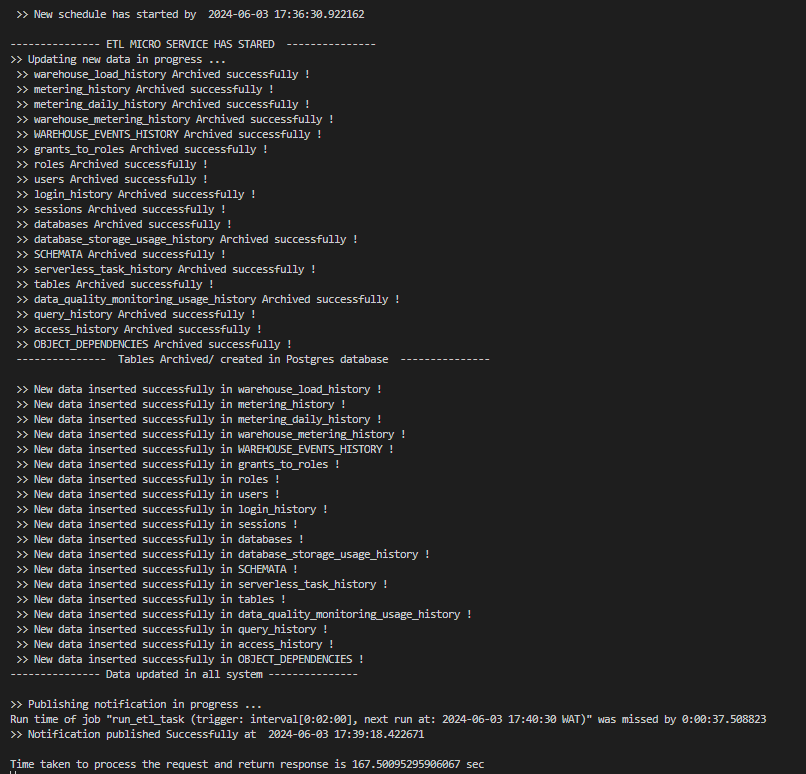
\includegraphics[width =1\linewidth ,height=12cm]{img/captures/etl/results.PNG}
    \caption{Exécution de l'ETL}
        \label{fig:result}
\end{figure}
\par Enfin, il stocke les nouvelles données dans les tables appriories et il publie un message dans le MQTT Broker pour notifier les utilisateurs du compte que les mise à jours sont faites avec succés comme l'indique la figure \textbf{\ref{fig:mqtt}}.

\begin{figure}[H]
    \centering
    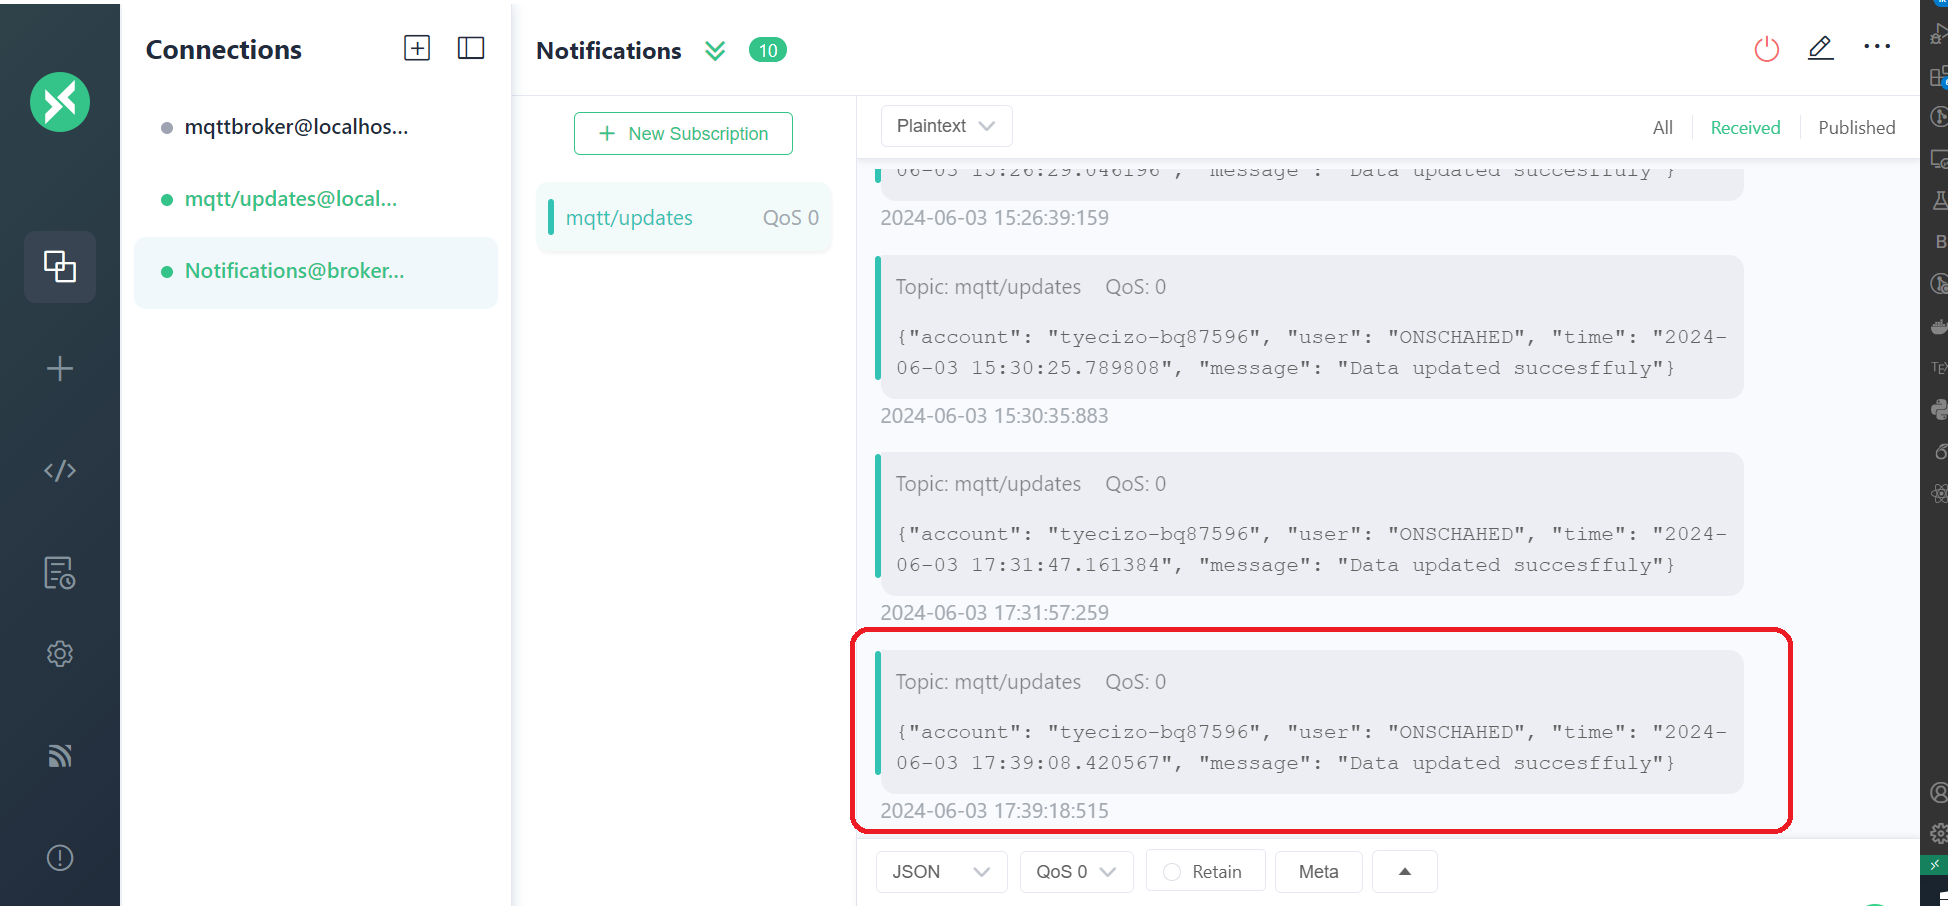
\includegraphics[width =1\linewidth]{img/captures/etl/mqtt.PNG}
    \caption{La publication du message dans MQTT Broker}
        \label{fig:mqtt}
\end{figure}

\subsection{Micro-service << Authentification\_Service >>}
\par Le micro-service << Authentification\_Service >> est responsable du système d'authentification de notre application 
\begin{itemize}
    \item \textbf{La liste des APIs:}
        \par La liste des APIs présents dans le micro-service d'authentification, documentée par Swagger, sont representés par la figure \textbf{\ref{fig:apiAuth}} suivante:
        \begin{figure}[H]
            \centering
            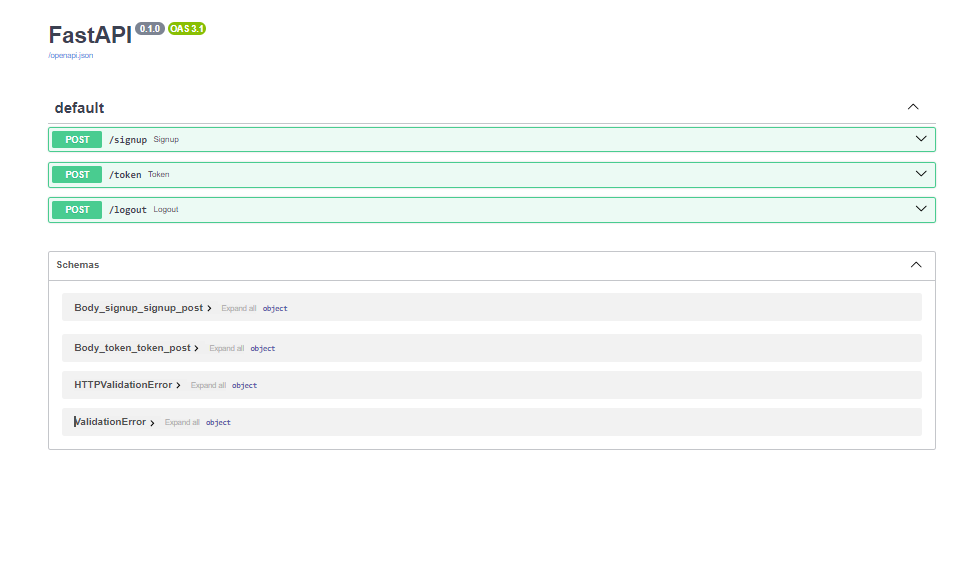
\includegraphics[width =1\linewidth, height=9cm]{img/captures/auth_apis.PNG}
            \caption{Liste des APIs du microservice <<Athentification\_service>> }
                \label{fig:apiAuth}
        \end{figure}
        \item \textbf{Interface de Création de compte <<Sign up>>:}
        \par L'interface de << Sign up>> est representée par la figure \textbf{\ref{fig:signup}} suivante:
        \begin{figure}[H]
            \centering
            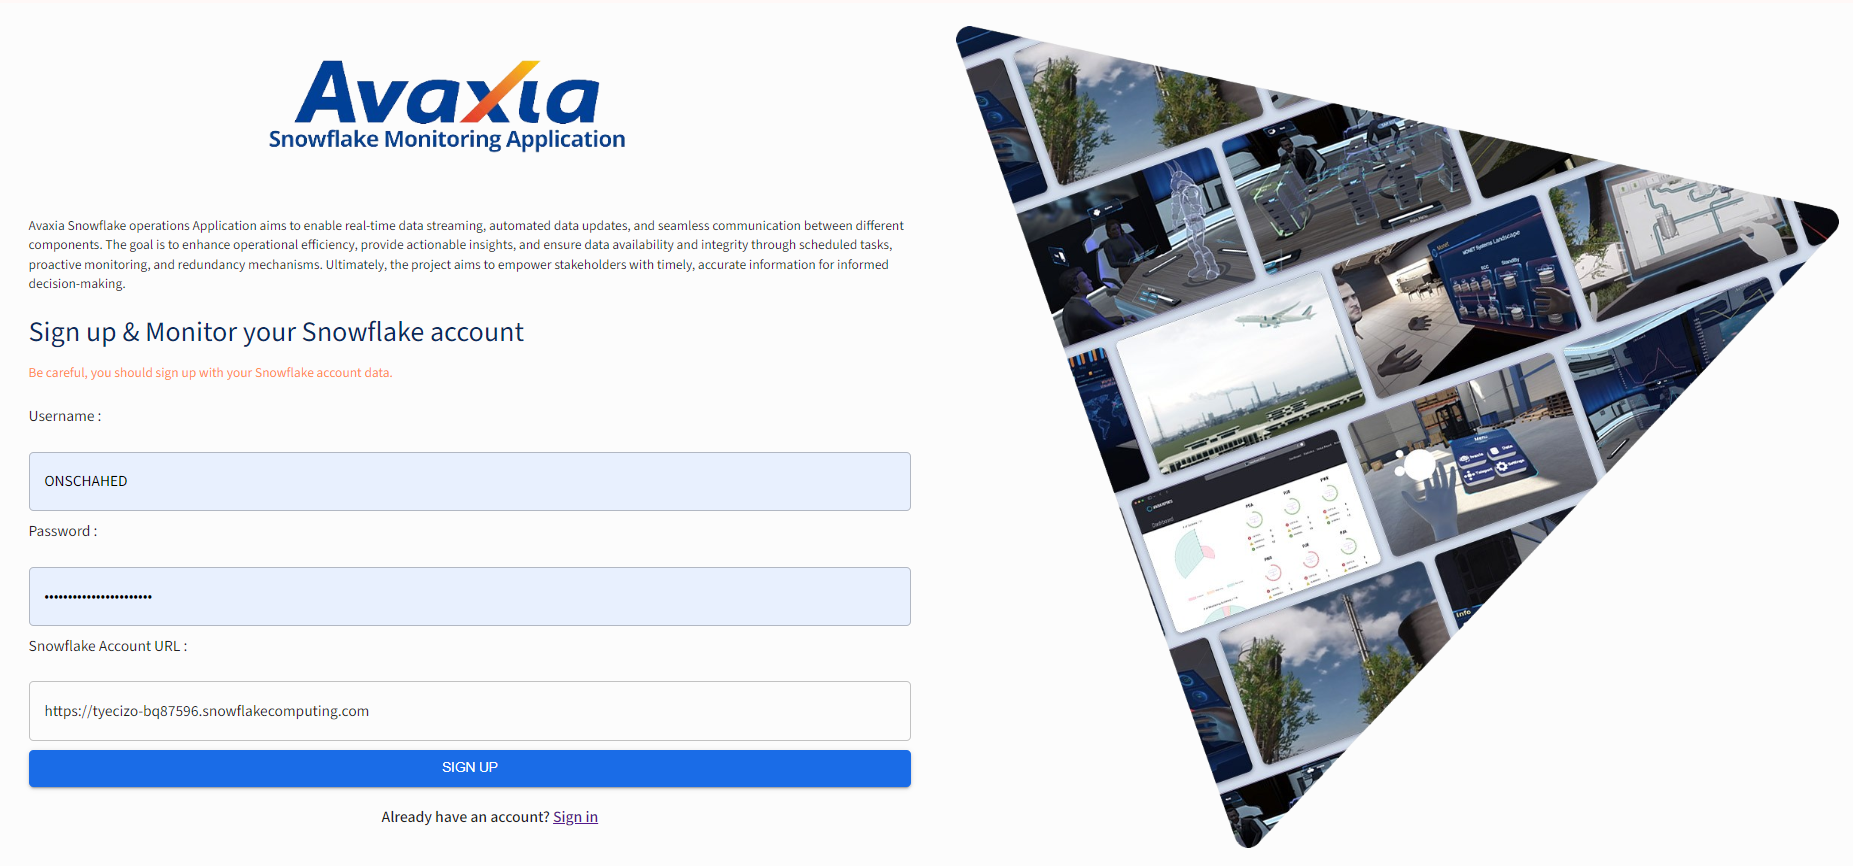
\includegraphics[width =1\linewidth, height=7cm]{img/captures/auth/signup.png}
            \caption{Interface de Création de compte <<Sign up>> }
                \label{fig:signup}
            \end{figure}
            \par Afin de créer un compte, l'utilisateur accède à cette interface en remplissant un formulaire d'inscription avec les données spécifiques à son compte Snowflake (nom d'utilisateur,mot de passe,l'url de connexion de son compte snowflake).
            Une fois l'utilisateur clique sur le bouton <<SINGUP>>, si les données sont valides: le système redirige l'utilisateur vers la page d'authentification. Sinon, il relance cette interface.
            \item \textbf{Interface d'authentification  <<Login>>:}
            \par L'interface de <<Login>> est representée par la figure \textbf{\ref{fig:login}} suivante:
            \begin{figure}[H]
                \centering
                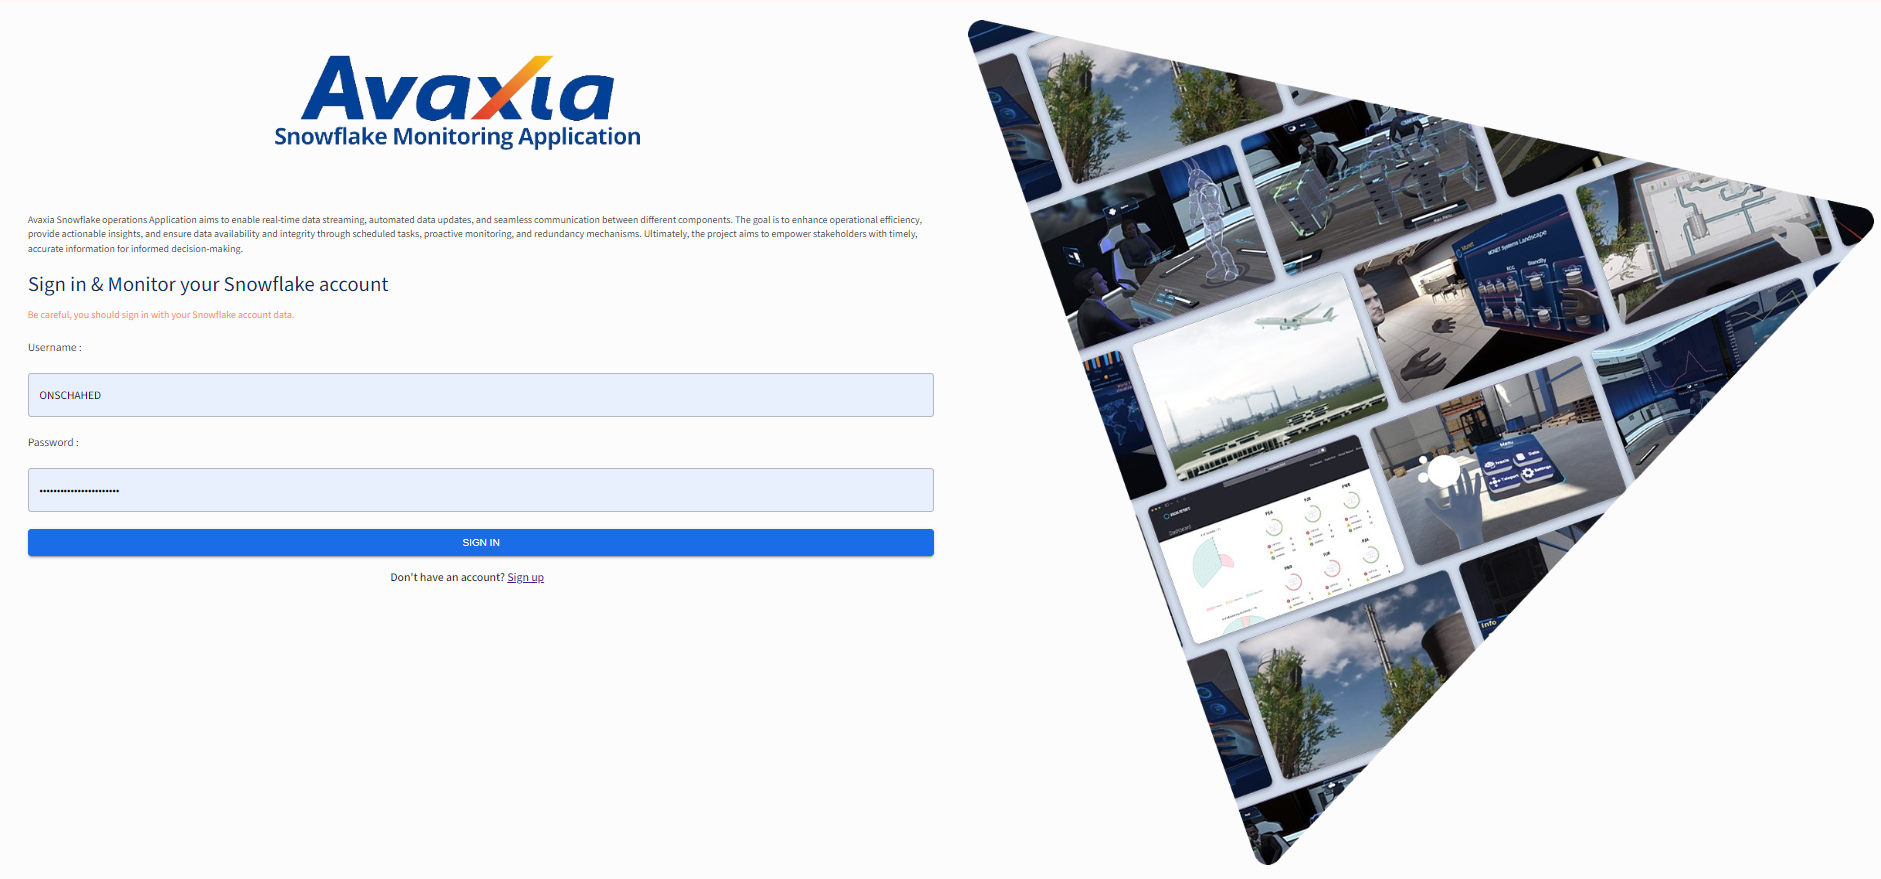
\includegraphics[width =1\linewidth , height=7cm]{img/captures/auth/login.png}
                \caption{Interface d'authentification  <<Login>>}
                    \label{fig:login}
                \end{figure}
                \par Pour accéder a son compte, l'utilisateur remplit le formulaire avec son <<nom d'utilisateur>> et <<mot de passe>>. Une fois les données sont valides, le système attribut une token d'accées à cet utilisateur et le redirige vers la page d'acceuil. Sinon, il relance la page de <<login>> en indiquant l'erreur.
                \par Si l'utilisateur est authentifié et clique sur le bouton <<Logout>>, indiqué dans la figure \textbf{\ref{fig:logout}}, il est redirigé vers l'interface de login automatiquement.
                \begin{figure}[H]
                    \centering
                    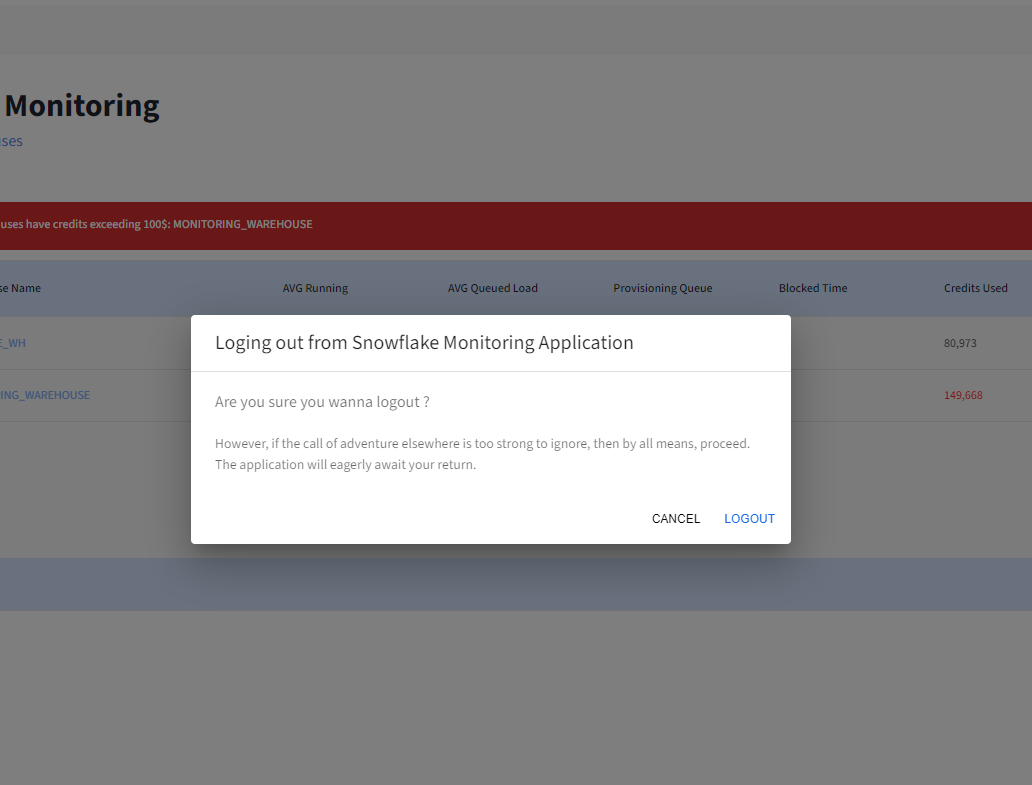
\includegraphics[width =1\linewidth]{img/captures/auth/logout.png}
                    \caption{ <<Logout>>}
                        \label{fig:logout}
                    \end{figure}s
            \end{itemize}
\par En conclusion, ce microservice joue un rôle essentiel dans la sécurité et la fiabilité de l'application. En implémentant le protocole OAuth 2.0, il garantit une authentification et une autorisation robustes, permettant aux utilisateurs de se connecter en toute sécurité et d'accéder uniquement aux fonctionnalités et aux données auxquelles ils sont autorisés. Ce service agit comme un gardien de la confidentialité et de l'intégrité des données, assurant que seuls les utilisateurs légitimes puissent interagir avec le système. 
\subsection{Micro-service << Warehouse\_Monitoring >>}
\par Le micro-service << Warehouse\_monitoring >> est le service chargé de la surveillance de l'utilisation des entrepôts de données Snowflake.
\begin{itemize}
    \item \textbf{La liste des APIs:}
        \par La liste des APIs présents dans ce micro-service, documentée par Swagger, sont representés par la figure \textbf{\ref{fig:apiWare}} suivante:
        \begin{figure}[H]
            \centering
            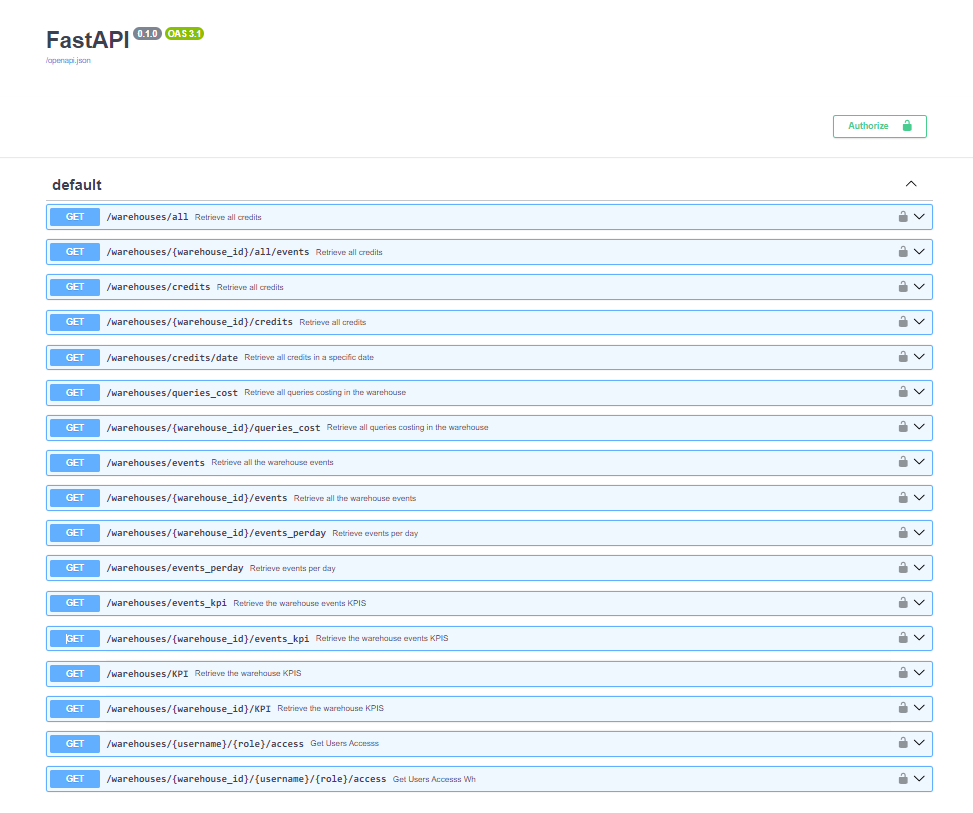
\includegraphics[width =1\linewidth]{img/captures/warehouses_apis.PNG}
            \caption{Liste des APIs du microservice <<Warehouse\_Monitoring>> }
                \label{fig:apiWare}
        \end{figure}

        \item \textbf{Interface de la liste des entrepôts de données:}
        \par L'interface de  de la liste des entrepôts de données est representée par la figure \textbf{\ref{fig:warehouse1}} suivante:
        \begin{figure}[H]
            \centering
            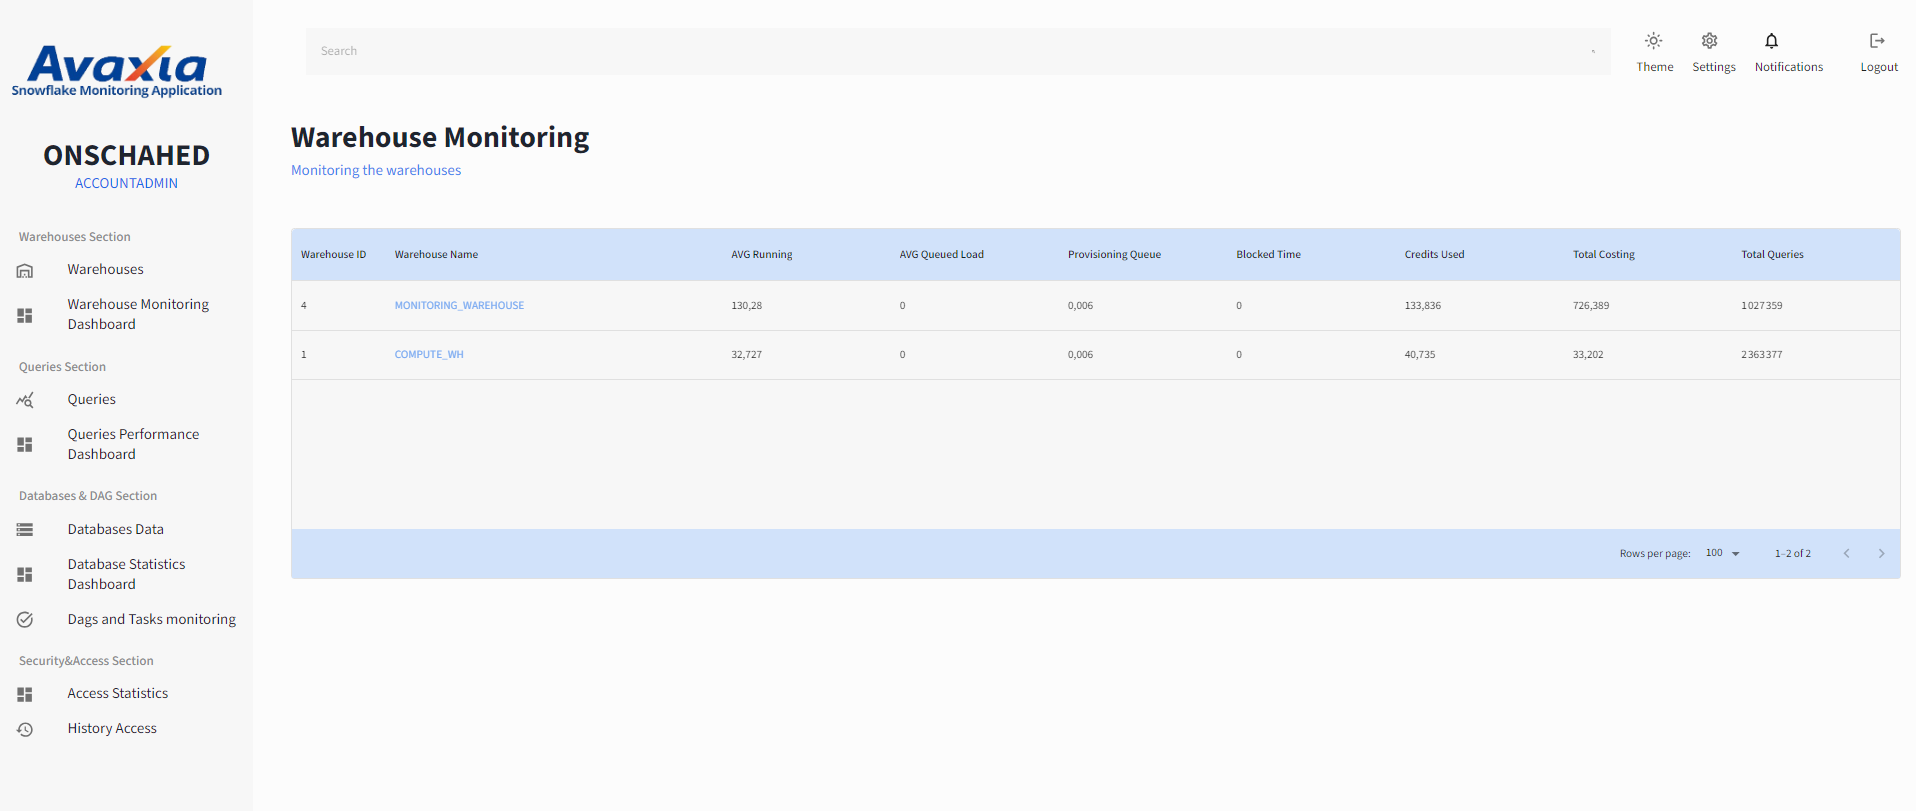
\includegraphics[width =1\linewidth]{img/captures/warehouse/liste.png}
            \caption{Interface de la liste des entrepôts de données}
                \label{fig:warehouse1}
            \end{figure}
            \par Le tableau présente des informations détaillées sur les différents entrepôts surveillés, notamment leur ID, leur nom, leurs métriques de performance (débit moyen, charge moyenne, file d'attente de provisionnement, temps bloqué, crédits utilisés, coût total) ainsi que le nombre total de requêtes. \\
            \item \textbf{Tableau de bord du surveillance des entrepôts des données}
            \par Les deux tableaux de bord du surveillance des entrepôts des données \textbf{<<Monitoring\_warehouse>>} et \textbf{<<Compute\_WH>>} sont representées par les deux figures \textbf{\ref{fig:warehouse2}} et \textbf{\ref{fig:warehouse3}}:
                \begin{figure}[H]
                    \centering
                    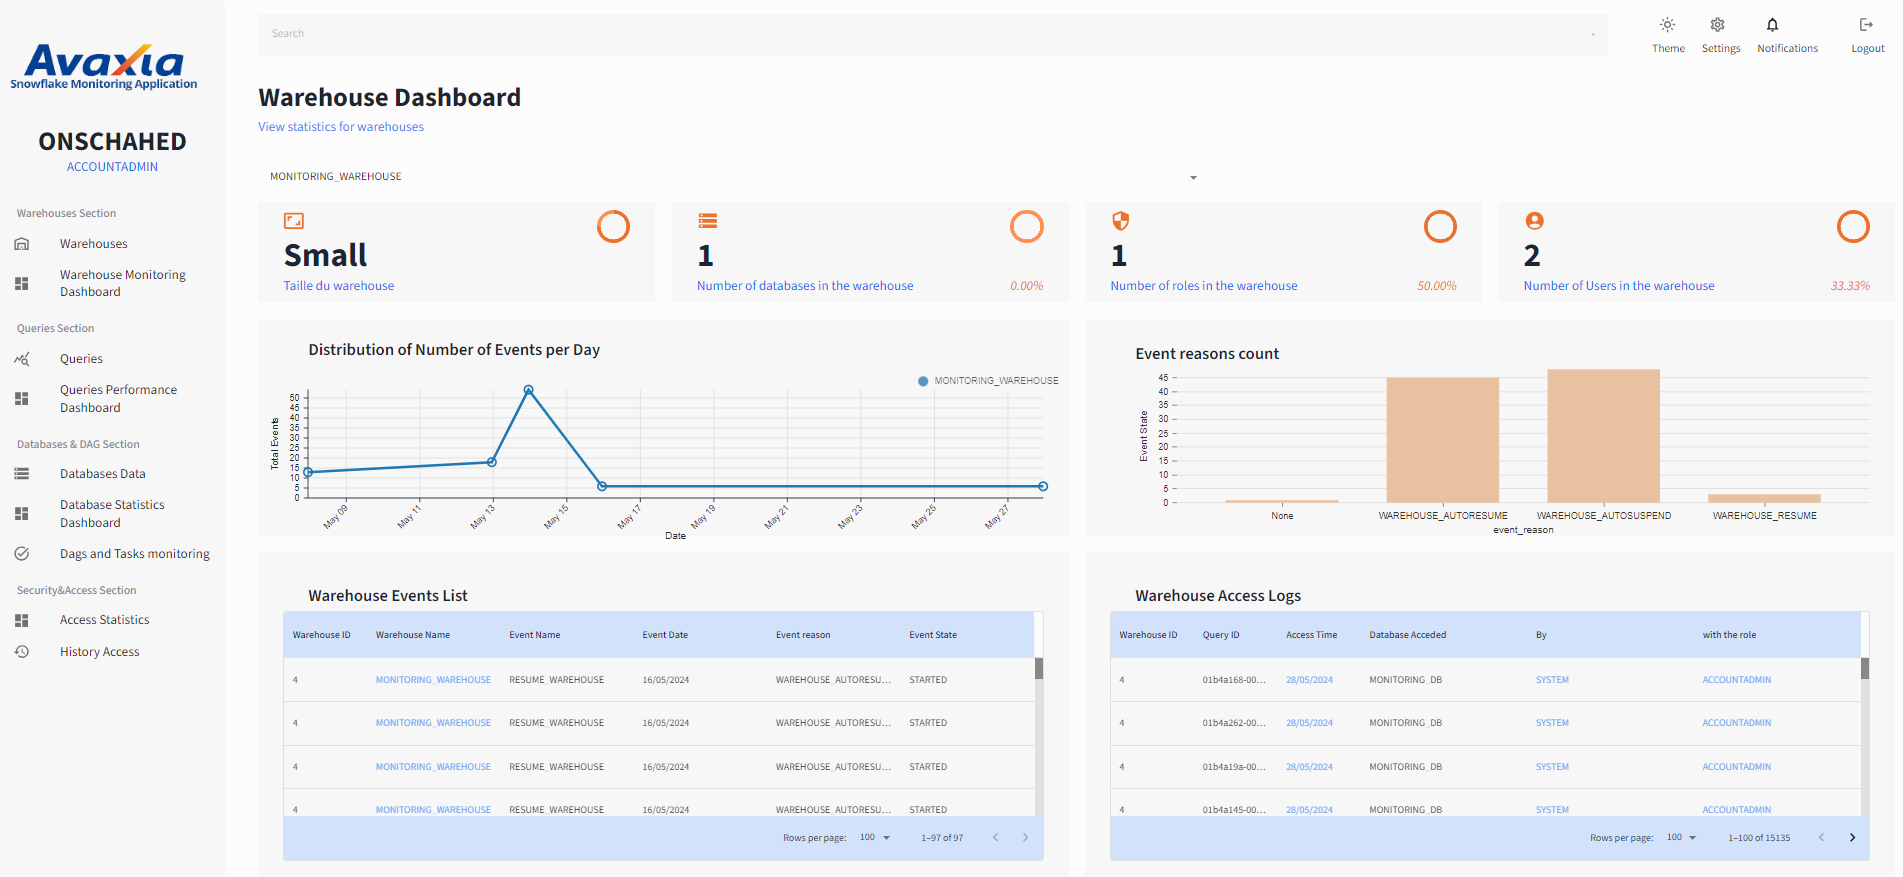
\includegraphics[width =1\linewidth]{img/captures/warehouse/warehouse_dash.png}
                    \caption{Tableau de bord du surveillance d l'entrepôts des données <<Monitoring\_warehouse>>}
                        \label{fig:warehouse2}
                \end{figure}
                \begin{figure}[H]
                    \centering
                    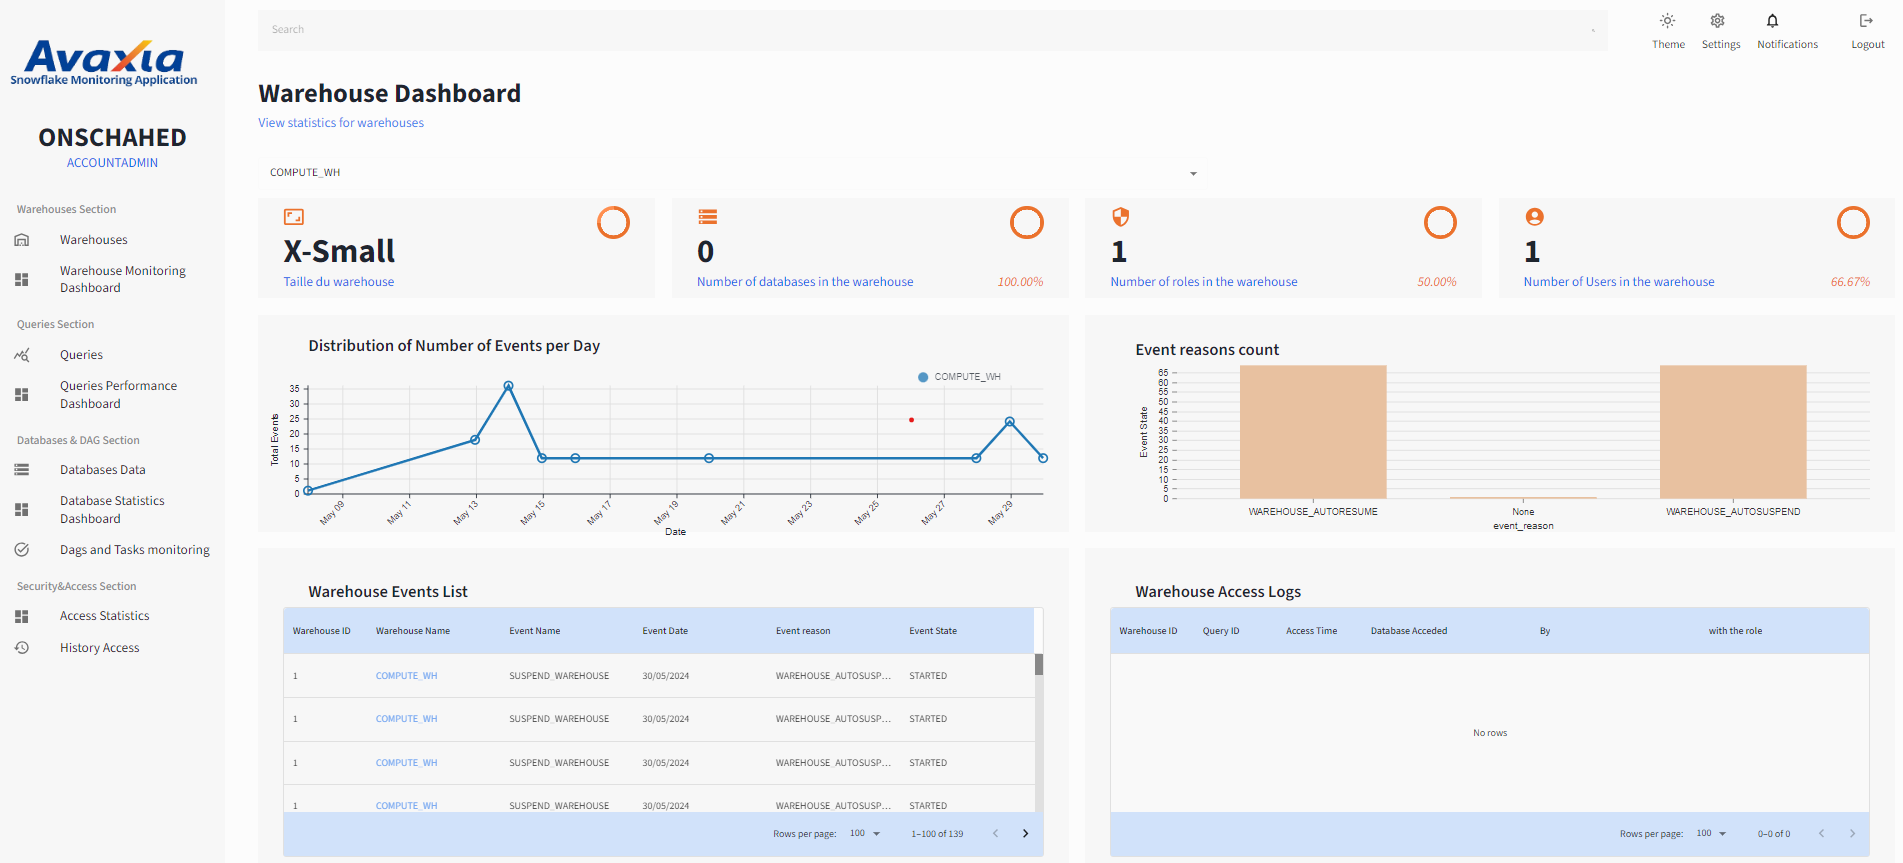
\includegraphics[width =1\linewidth]{img/captures/warehouse/compute.png}
                    \caption{Tableau de bord du surveillance d l'entrepôts des données <<Compute\_WH>>}
                        \label{fig:warehouse3}
                \end{figure}
                \par Ces tableaux de bord des entrepôts Snowflake offrent un aperçu complet des activités et de l'utilisation de l'infrastructure de données. Ils présentent des informations clés sur la taille, la composition et l'utilisation des entrepôts, notamment le nombre de bases de données, nombre des événments effectuées dans l'entrepôt ainsi que le nombre de rôles et d'utilisateurs.
                
                 
            \item \textbf{Changement des variables globaux}
            \par Le changement des paramétres globaux peut reflecter les vues de ce micro service, une fenêtre s'affiche lorsqu'on clique sur le bouton <<Settings>> du topbar.
            Selon les besoins de l'utilisateur/administrateur les changements qui peuvent être appliqueés :
                \begin{enumerate}
                    \item[-] \textbf{Changement du rôle d'utilisateur/Administrateur:}
                    \begin{figure}[H]
                        \centering
                        \begin{tabular}[b]{c}
                        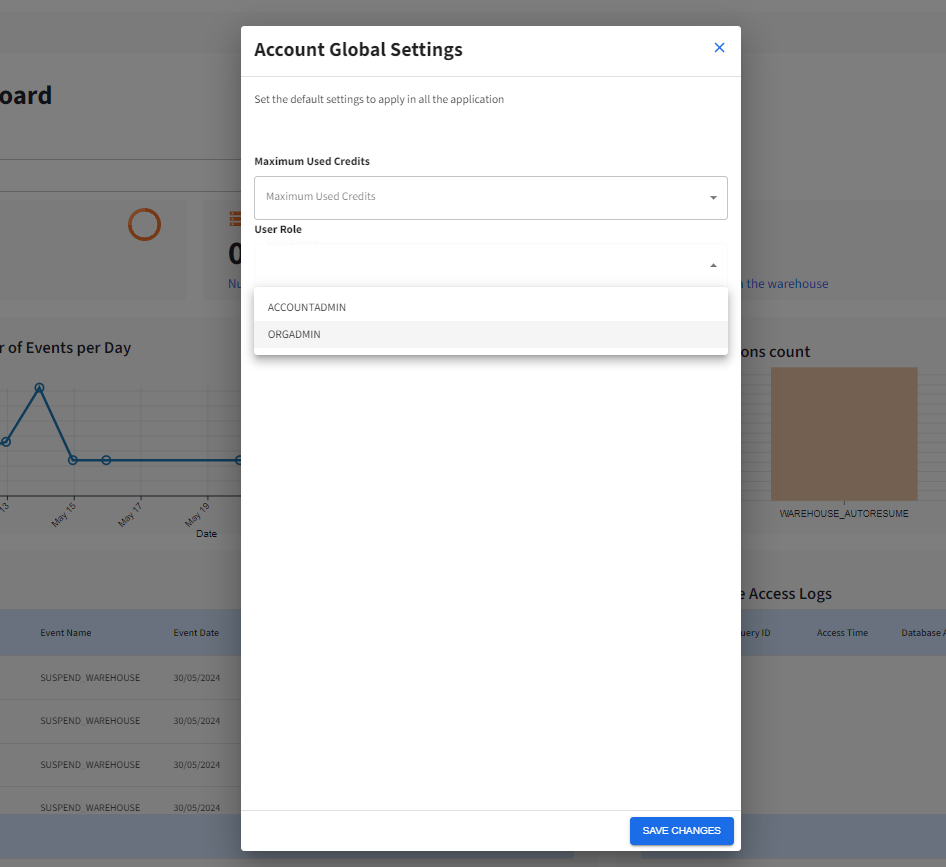
\includegraphics[width=.3\linewidth, height=5cm]{img/captures/warehouse/global_set_role.png} \\
                        
                        \end{tabular} 
                        \begin{tabular}[b]{c}
                        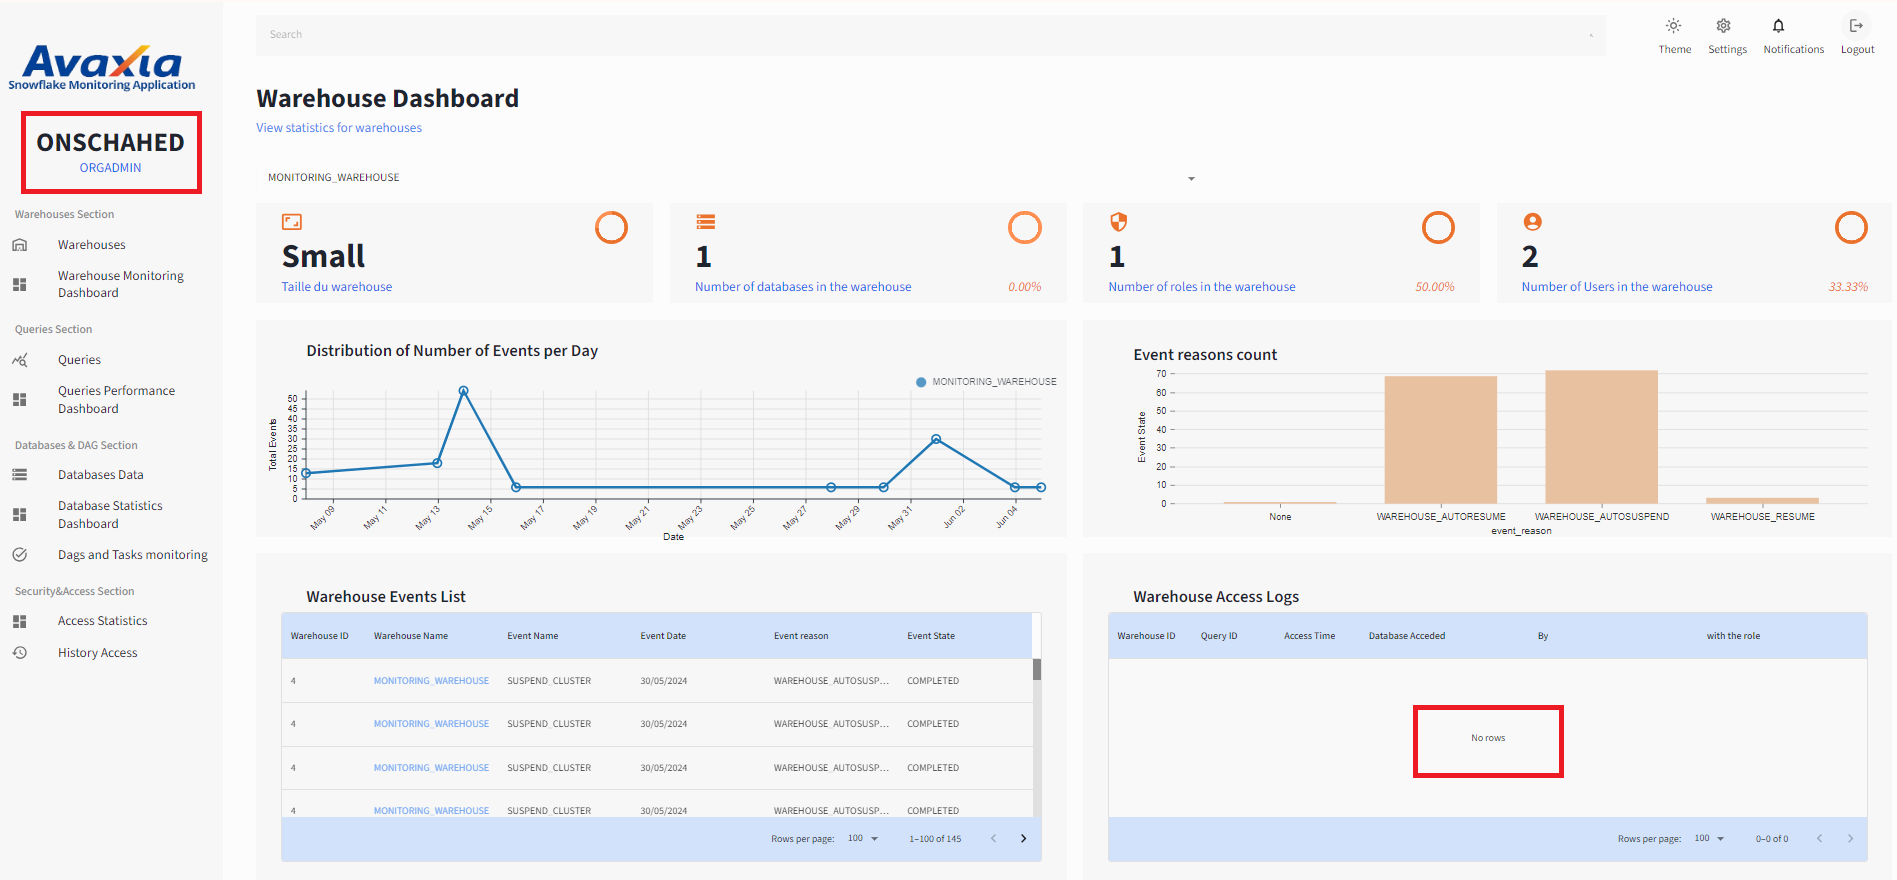
\includegraphics[width=.6\linewidth, height=5cm]{img/captures/warehouse/sysorg.png} \\
                        
                        \end{tabular}
                        \caption{Changement du role de l'utilisateur de <<ACCOUNT ADMIN>> vers <<ORGADMIN>>                    }
                    \end{figure}
                    \par Lorsque l'utilisateur  modifit les paramètres globaux, telque le rôle de compte utilisateur, les journaux d'accès aux entrepôts ne sont plus affichés dans cette interface. Cela signifie que les administrateurs doivent être conscients que certaines informations peuvent ne pas être visibles dans certaines configurations.
                    \item[-] \textbf{Changement du seuil maximum des crédits d'utilisation:}
                    \begin{figure}[H]
                        \centering
                        \begin{tabular}[b]{c}
                        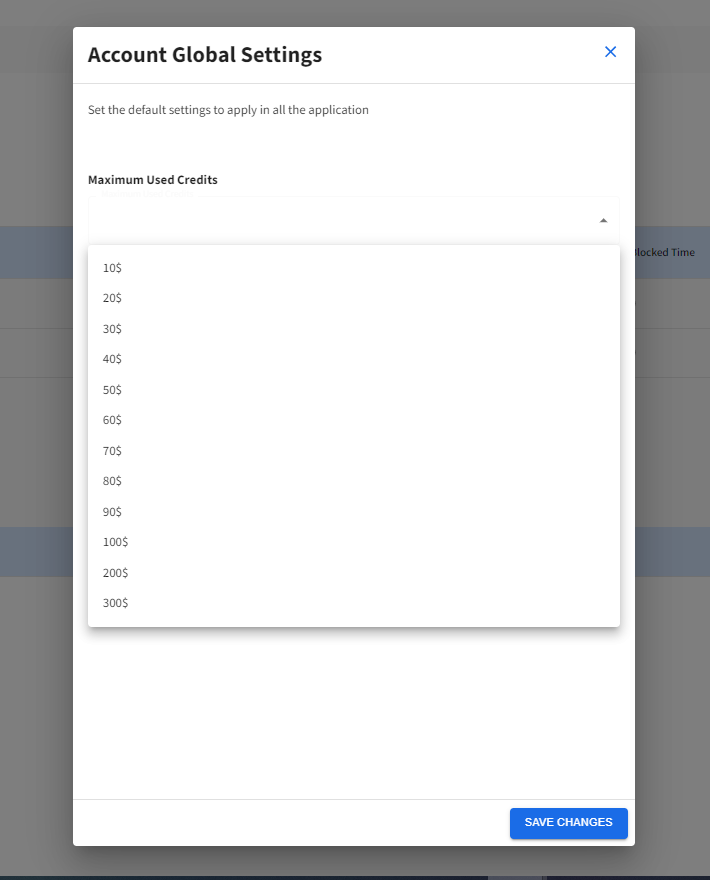
\includegraphics[width=.2\linewidth, height=5.5cm]{img/captures/warehouse/global_set_credits.png} \\
                        
                        \end{tabular} 
                        \begin{tabular}[b]{c}
                        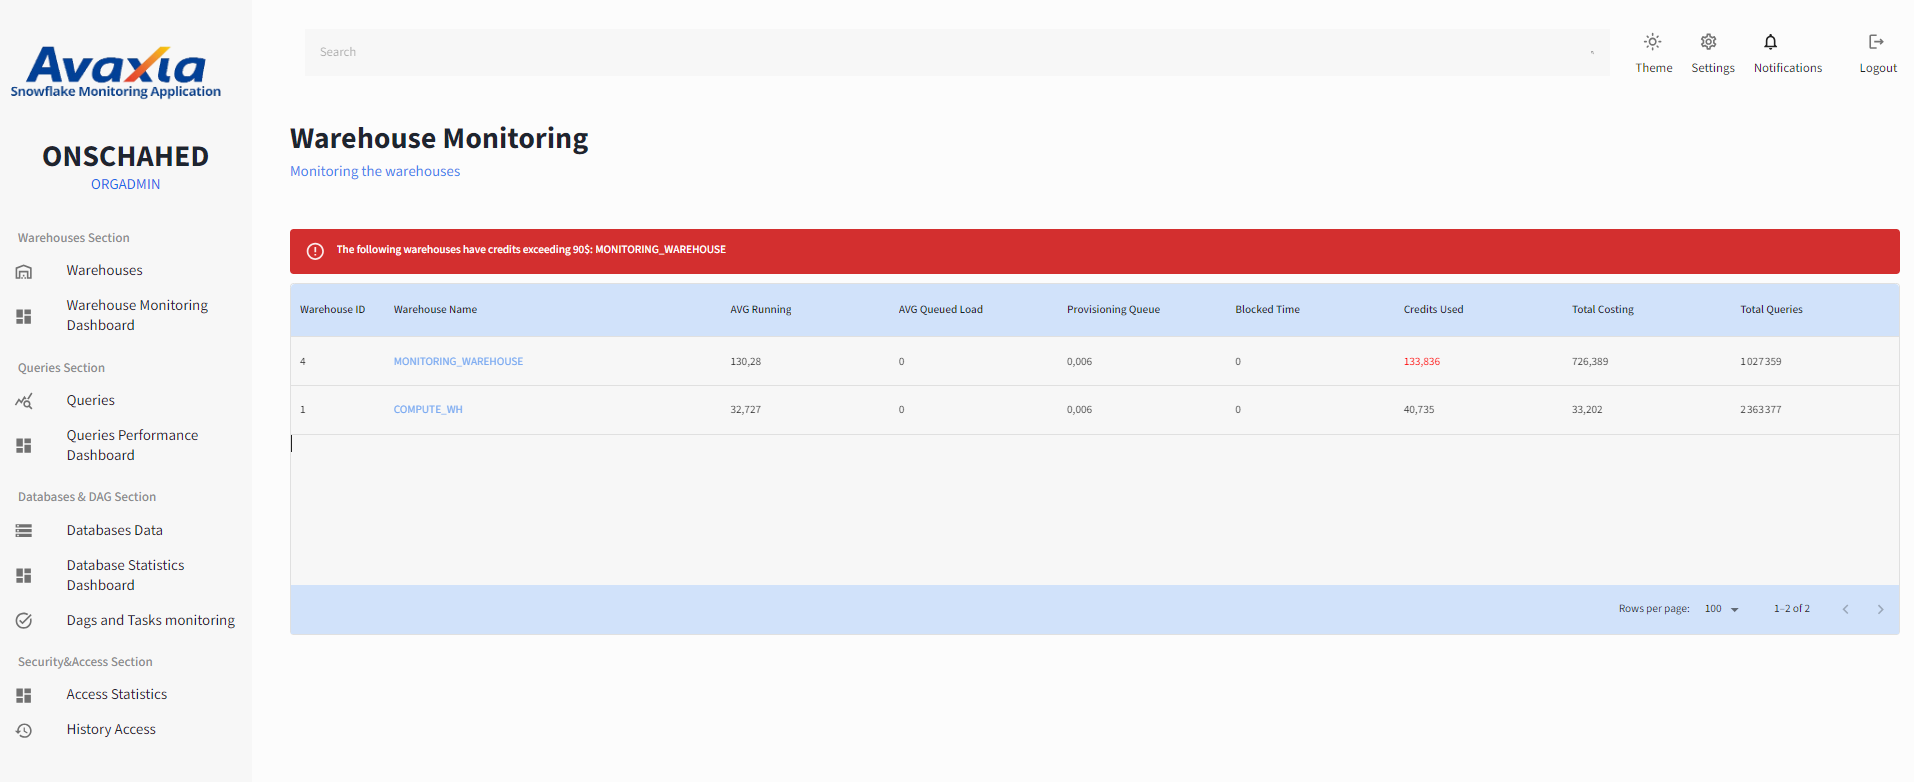
\includegraphics[width=.7\linewidth, height=5.5cm]{img/captures/warehouse/90.png} \\
                        
                        \end{tabular}
                        \caption{Changement de seuil de credits vers <<90\$>>                    }
                    \end{figure}
                    \par Lorsque l'utilisateur modifie les paramètres globaux, notamment le seuil de crédits maximum utilisés,
                     une notification permanente devrait être affichée si les crédits utilisés de l'un des entrepôt de donneés à dépacer cette seuil 
                     pour informer l'utilisateur de cette malveillance.
            \end{enumerate}

\end{itemize}
\par Dans l'ensemble, ce microservice offre une visibilité essentielle sur les performances et l'utilisation des entrepôts, facilitant la prise de décisions éclairées pour l'infrastructure de données.
\subsection{Micro-service << Query\_Performance >>}
\par Le micro-service << Query\_Performance  >> est le service chargé de la surveillance des requêtes SQL effectuées au sein du compte Snowflake.
\begin{itemize}
    \item \textbf{La liste des APIs:}
        \par La liste des APIs présents dans ce micro-service, documentée par Swagger, sont representés par la figure \textbf{\ref{fig:apiquery}} suivante:
        \begin{figure}[H]
            \centering
            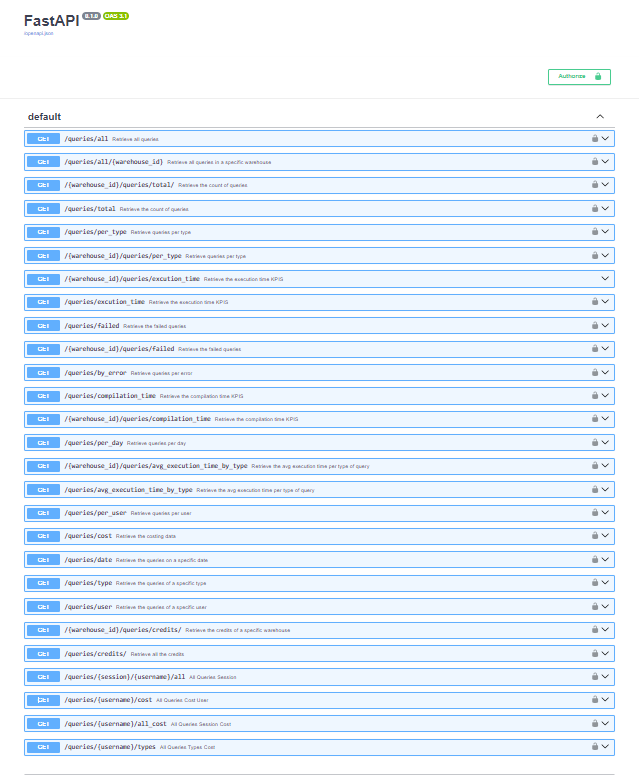
\includegraphics[width =1\linewidth]{img/captures/queries_apis.PNG}
            \caption{Liste des APIs du microservice <<Warehouse\_Monitoring>> }
                \label{fig:apiquery}
        \end{figure}

        \item \textbf{Interface de l'historique des requêtes de l'utilisateur:}
        \par L'interface de la liste des entrepôts de données est representée par la figure \textbf{\ref{fig:listqueries}} suivante:
        \begin{figure}[H]
            \centering
            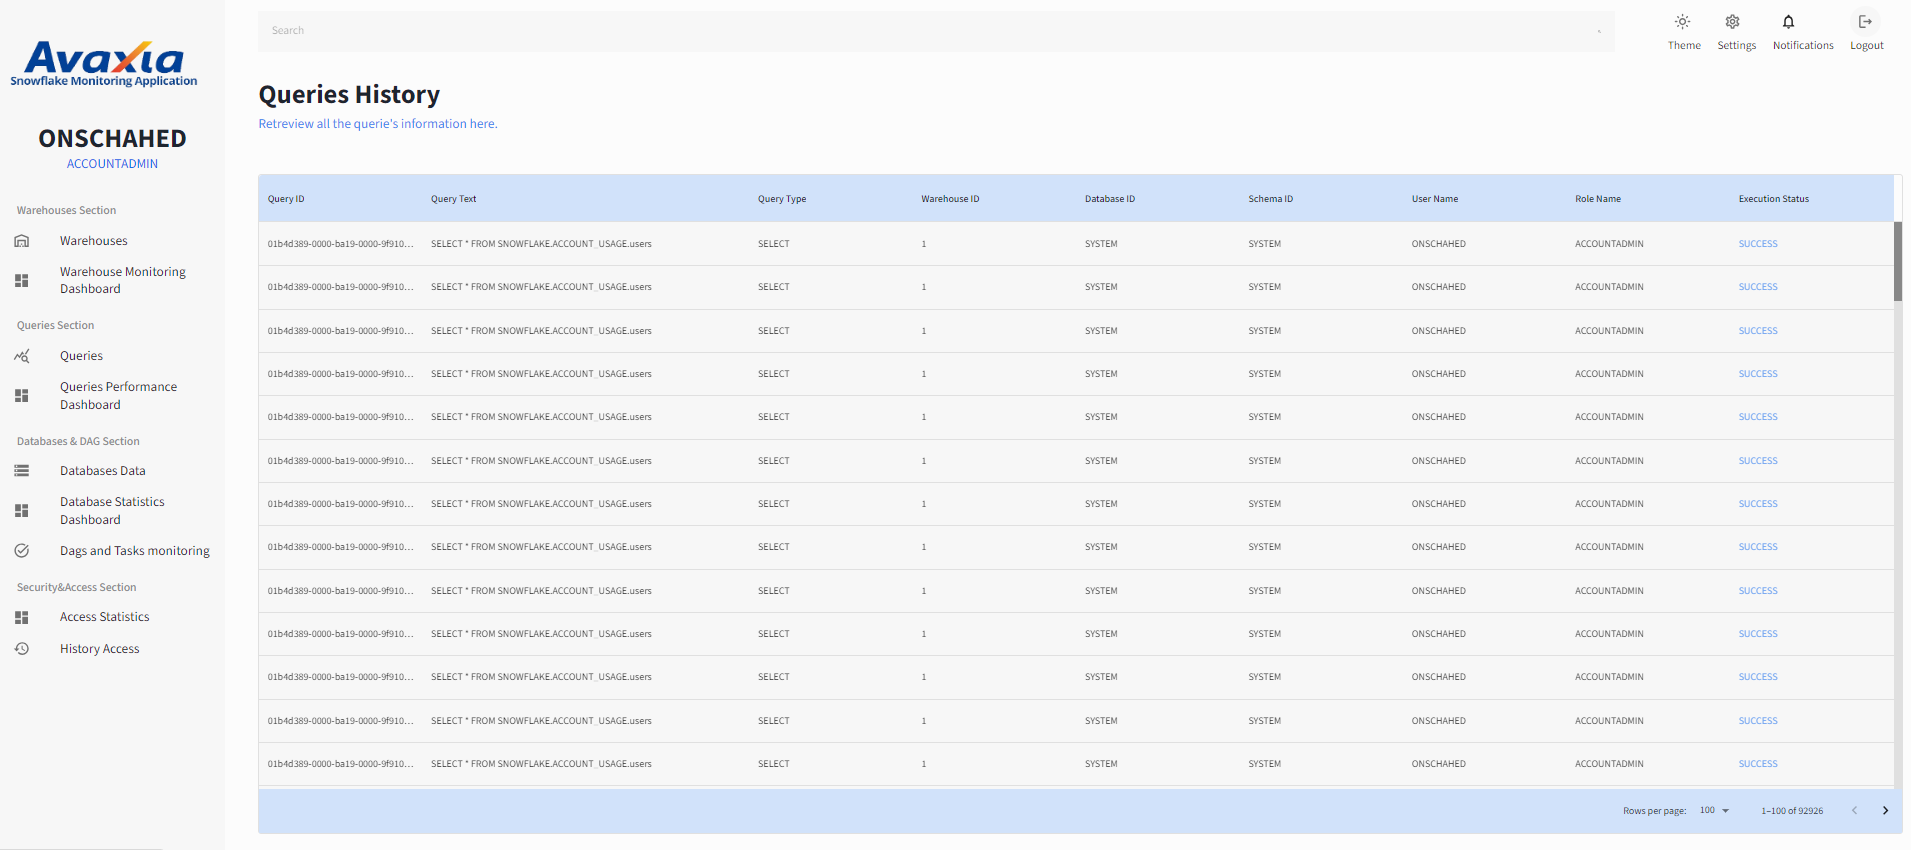
\includegraphics[width =1\linewidth]{img/captures/queries/queries_list.png}
            \caption{Interface de la liste des entrepôts de données}
                \label{fig:listqueries}
            \end{figure}
            \par Cette vue représente l'historique des requêtes dans l'application de surveillance Snowflake.
             Elle fournit un aperçu détaillé de chaque requête exécutée. \\ 
             Cet historique permet aux administrateurs de surveiller en détail les requêtes exécutées afin de pouvoir identifier les éventuels problèmes liés aux ces derniers dans le compte Snowflake en question.
            \item \textbf{Tableaux de bord du surveillance des Requêtes SQL}
            \begin{enumerate}
                \item[-] \textbf{Les informations générale sur la totalité des requêtes dans le compte de l'utilisateur:  }
                    \par La figure \textbf{\ref{fig:queriesglob}} illustre le tableau de bord global des requêtes SQL du compte Snowflake:
                    \begin{figure}[H]
                        \centering
                        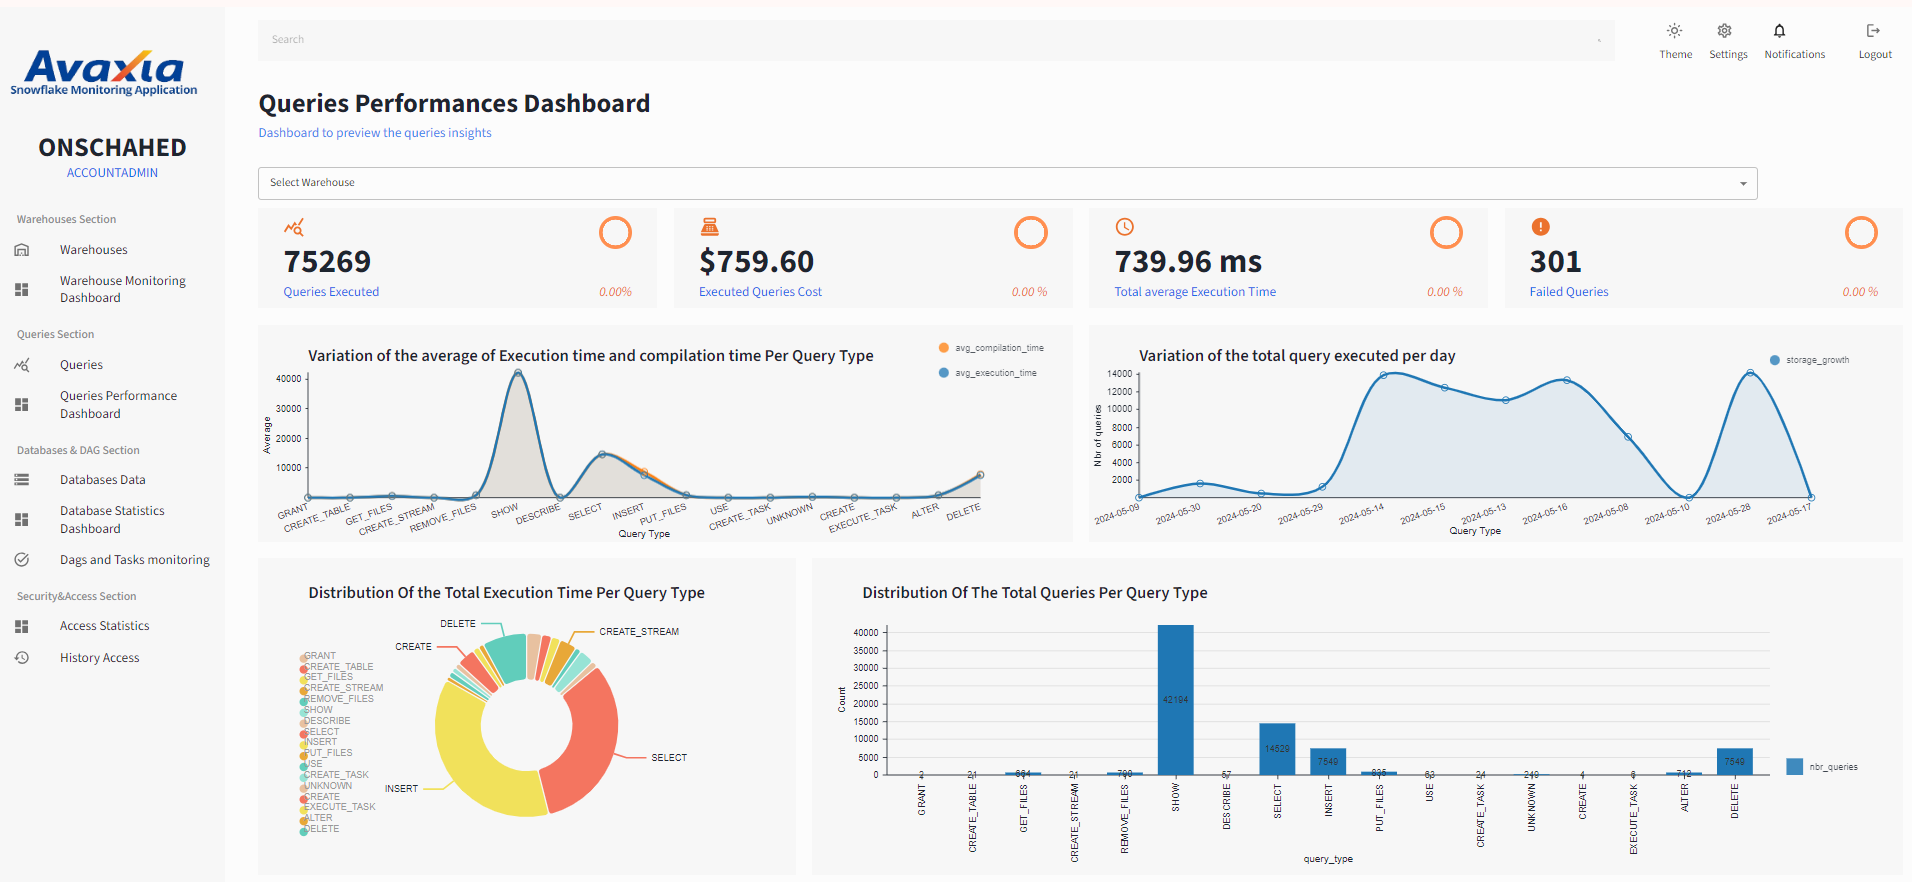
\includegraphics[width =1\linewidth]{img/captures/queries/global_queries_dash.png}
                        \caption{Tableau de bord du surveillance des entrepôts des données}
                            \label{fig:queriesglob}
                    \end{figure}
                    \item[-] \textbf{Selection  de l'entrepôts des données appriori:}
                    
                    \par Une fois l'utilisateur selectionne un entrepôt de données, depuis la liste de ces entrepôts, qui s'affiche en cliquant sur la liste déroulante <<select warehouse>> comme l'indique la figure \textbf{\ref{fig:select}}, les données spécifique à cet entrepôt vont être affichées.
                    \begin{figure}[H]
                        \centering
                        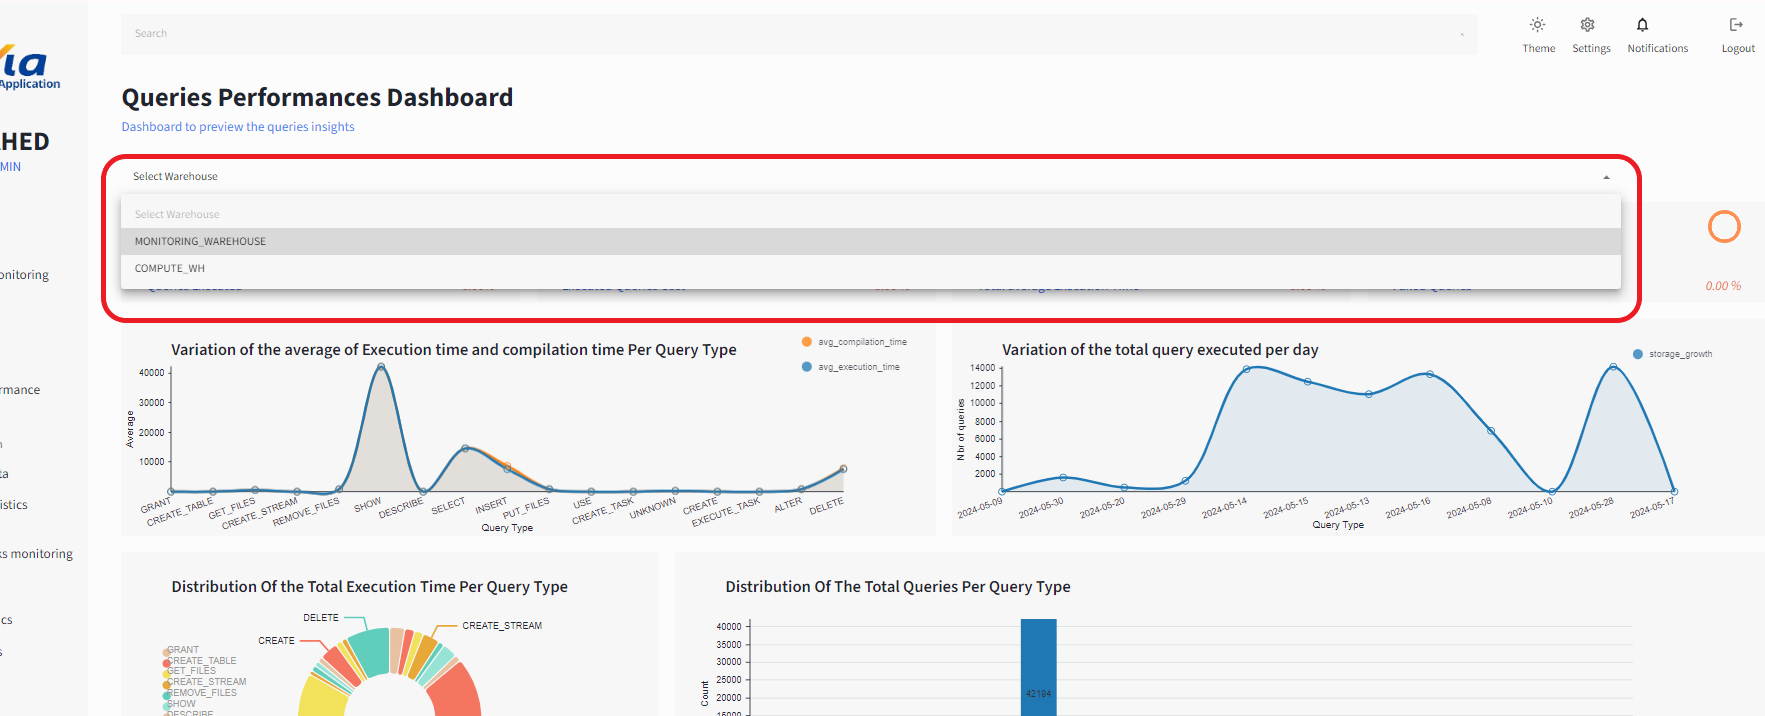
\includegraphics[width =1\linewidth]{img/captures/queries/queries_selection_warehouse.png}
                        \caption{Tableau de bord du surveillance des entrepôts des données}
                            \label{fig:select}
                    \end{figure}
                    \par La figure \textbf{\ref{fig:queriesdash1}} illustre le tableau de bord de l'entrepôt <<Monitoring\_Warehouse>>:
                    \begin{figure}[H]
                        \centering
                        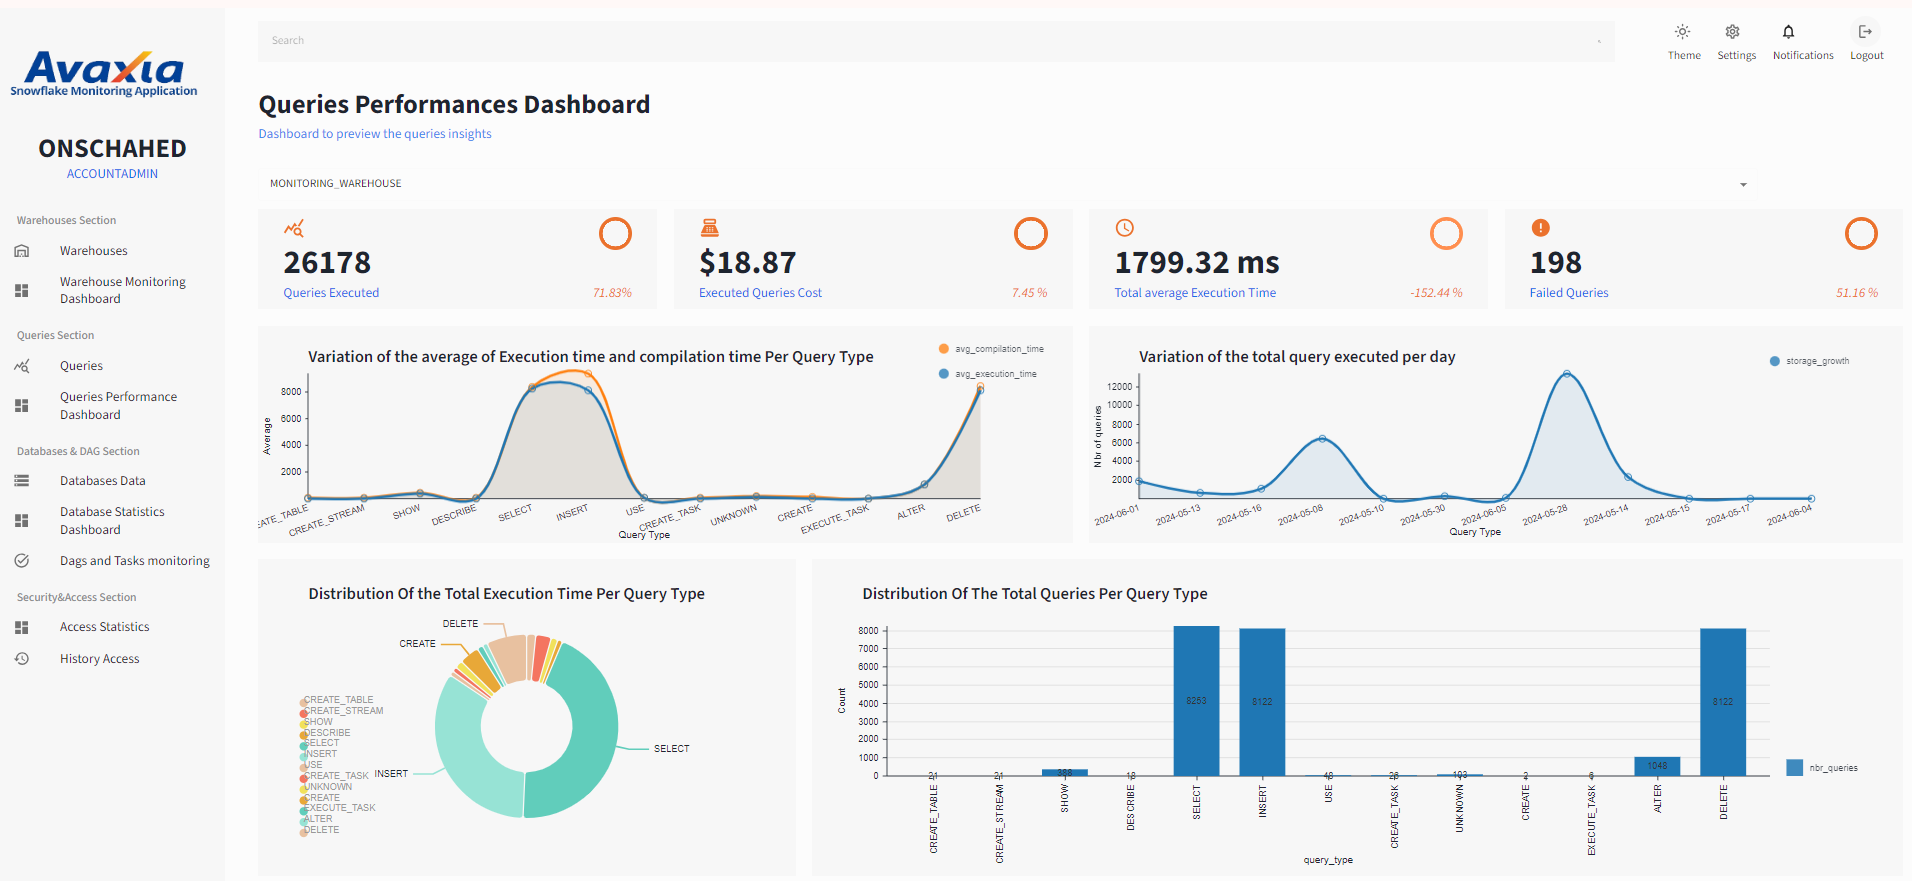
\includegraphics[width =1\linewidth]{img/captures/queries/monitoring_dash.png}
                        \caption{Tableau de bord du surveillance de l'entrepôt des données <<Monitoring\_Warehouse>> }
                            \label{fig:queriesdash1}
                    \end{figure}
                    \par La figure \textbf{\ref{fig:queriesdash2}} illustre le tableau de bord de l'entrepôt <<Compute\_WH>>:
                    \begin{figure}[H]
                        \centering
                        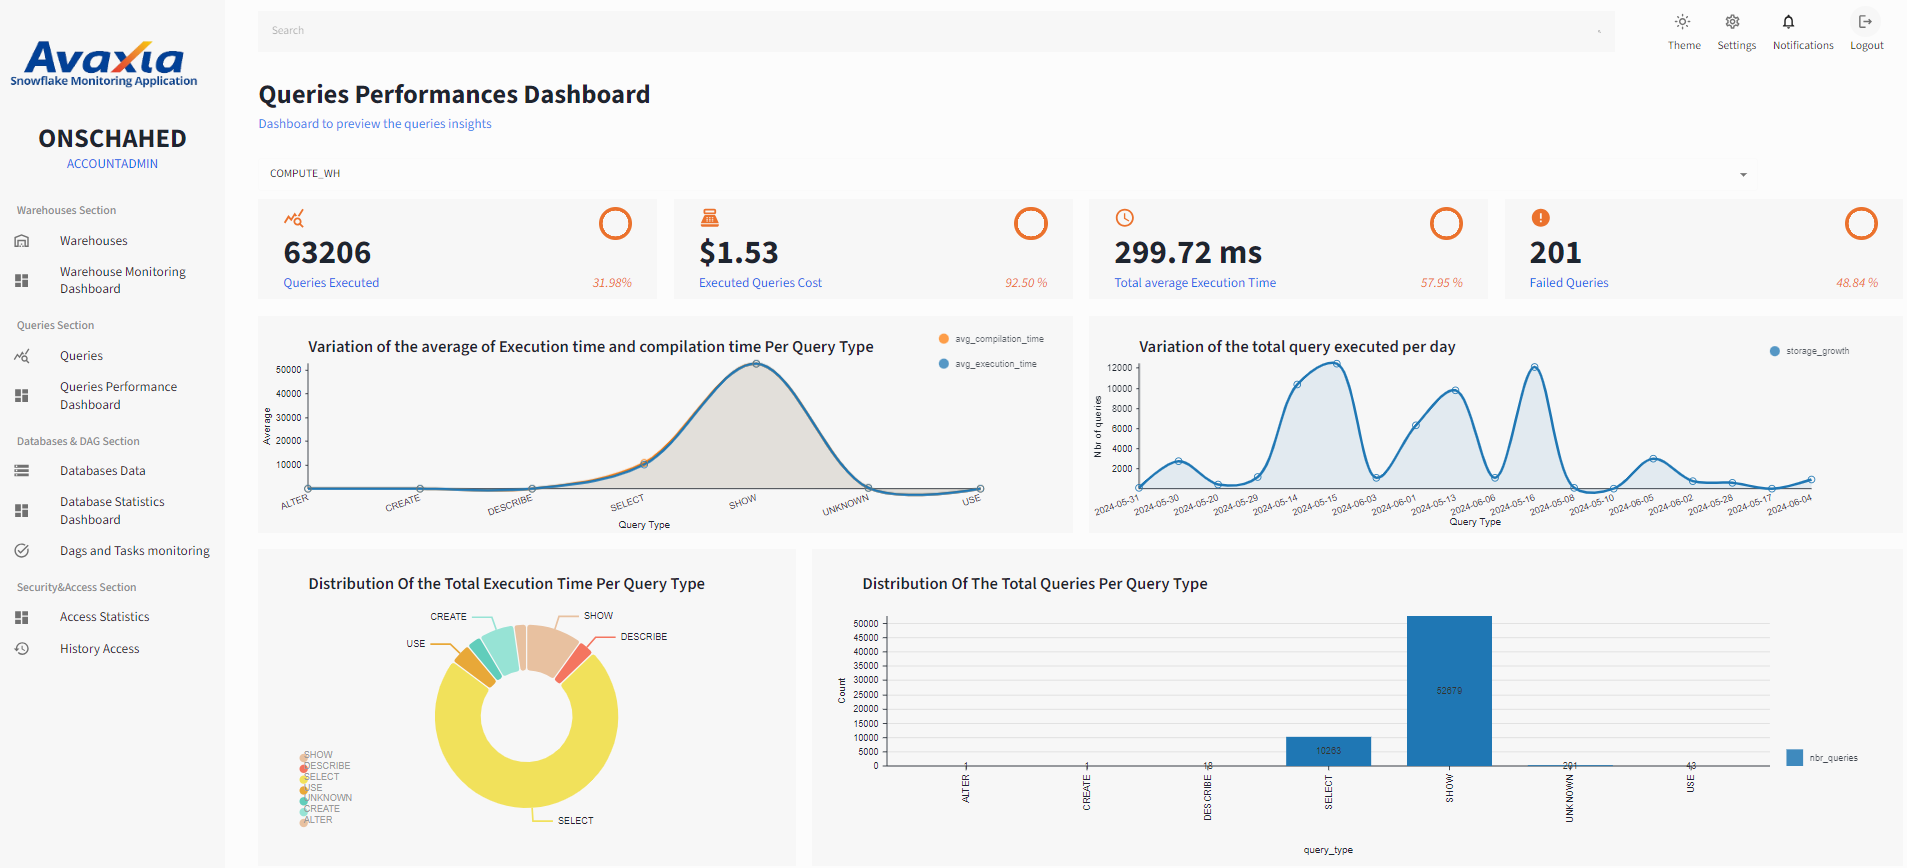
\includegraphics[width =1\linewidth]{img/captures/queries/compute_dash.png}
                        \caption{Tableau de bord du surveillance de l'entrepôt des données <<Compute\_WH>>}
                            \label{fig:queriesdash2}
                    \end{figure}
                    \par ces tableaux de bord présentent des indicateurs clés sur les requêtes exécutées, tels que le nombre total de requêtes, le coût total, le temps d'exécution moyen et le taux de requêtes en échec. Cette vision synthétique permet aux administrateurs d'avoir une compréhension globale des performances.
                    \\ Les graphiques complémentaires apportent une analyse approfondie des tendances par type de requête. Ils montrent la variation du temps d'exécution et de compilation, ainsi que la répartition du nombre total de requêtes et du temps d'exécution par type de requête. Cette granularité permet d'identifier les domaines à optimiser pour améliorer l'efficacité du système.
            \end{enumerate}

\end{itemize}
\par Le service  << Query\_Performance >> constitue un outil essentiel pour les équipes en charge de l'exploitation et 
de l'optimisation de l'infrastructure Snowflake. Il offre une visibilité complète sur les activités de requêtes, 
permettant de prendre des décisions éclairées afin d'améliorer la fiabilité, les performances et la rentabilité globale du système.
\subsection{Micro-service << Databases\_Statistics >>}
\par Le micro-service << Databases\_Statistics >> est le service chargé de la surveillance des base de données créees au sein du compte Snowflake.
\begin{itemize}
    \item \textbf{La liste des APIs :}
        \par La liste des APIs présents dans ce micro-service, documentée par Swagger, sont representés par la figure \textbf{\ref{fig:apiData}} suivante:
        \begin{figure}[H]
            \centering
            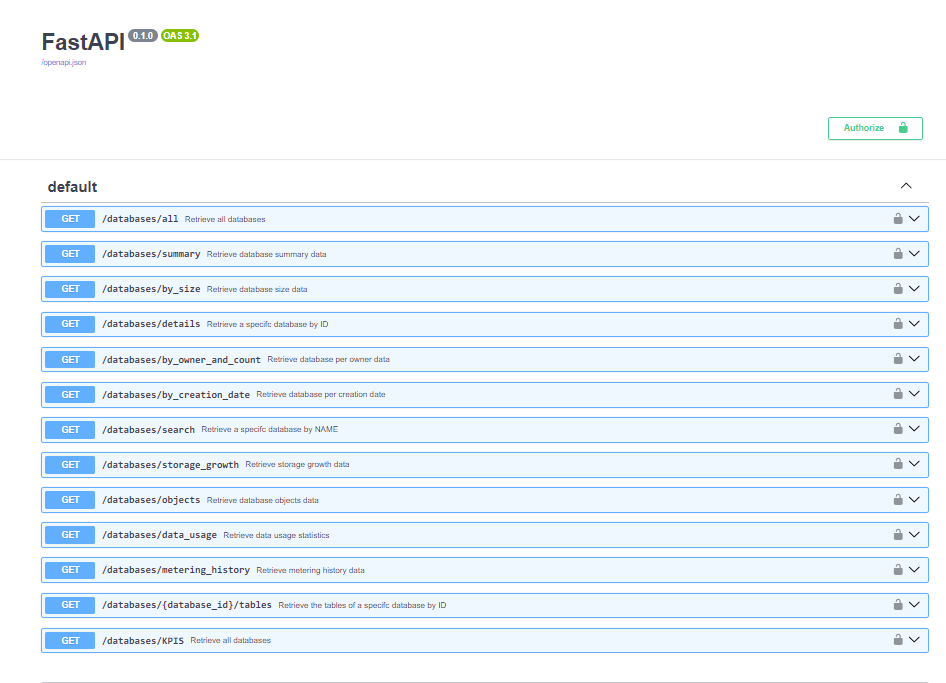
\includegraphics[width =1\linewidth]{img/captures/database_apis.PNG}
            \caption{Liste des APIs du microservice<< Databases\_Statistics >> }
                \label{fig:apiData}
        \end{figure}

        \item \textbf{La liste des bases de données et ses différents schémas :}
        \par L'interface de la liste des bases de données et ses différents schémas est representée par la figure \textbf{\ref{fig:dblist}} suivante:
        \begin{figure}[H]
            \centering
            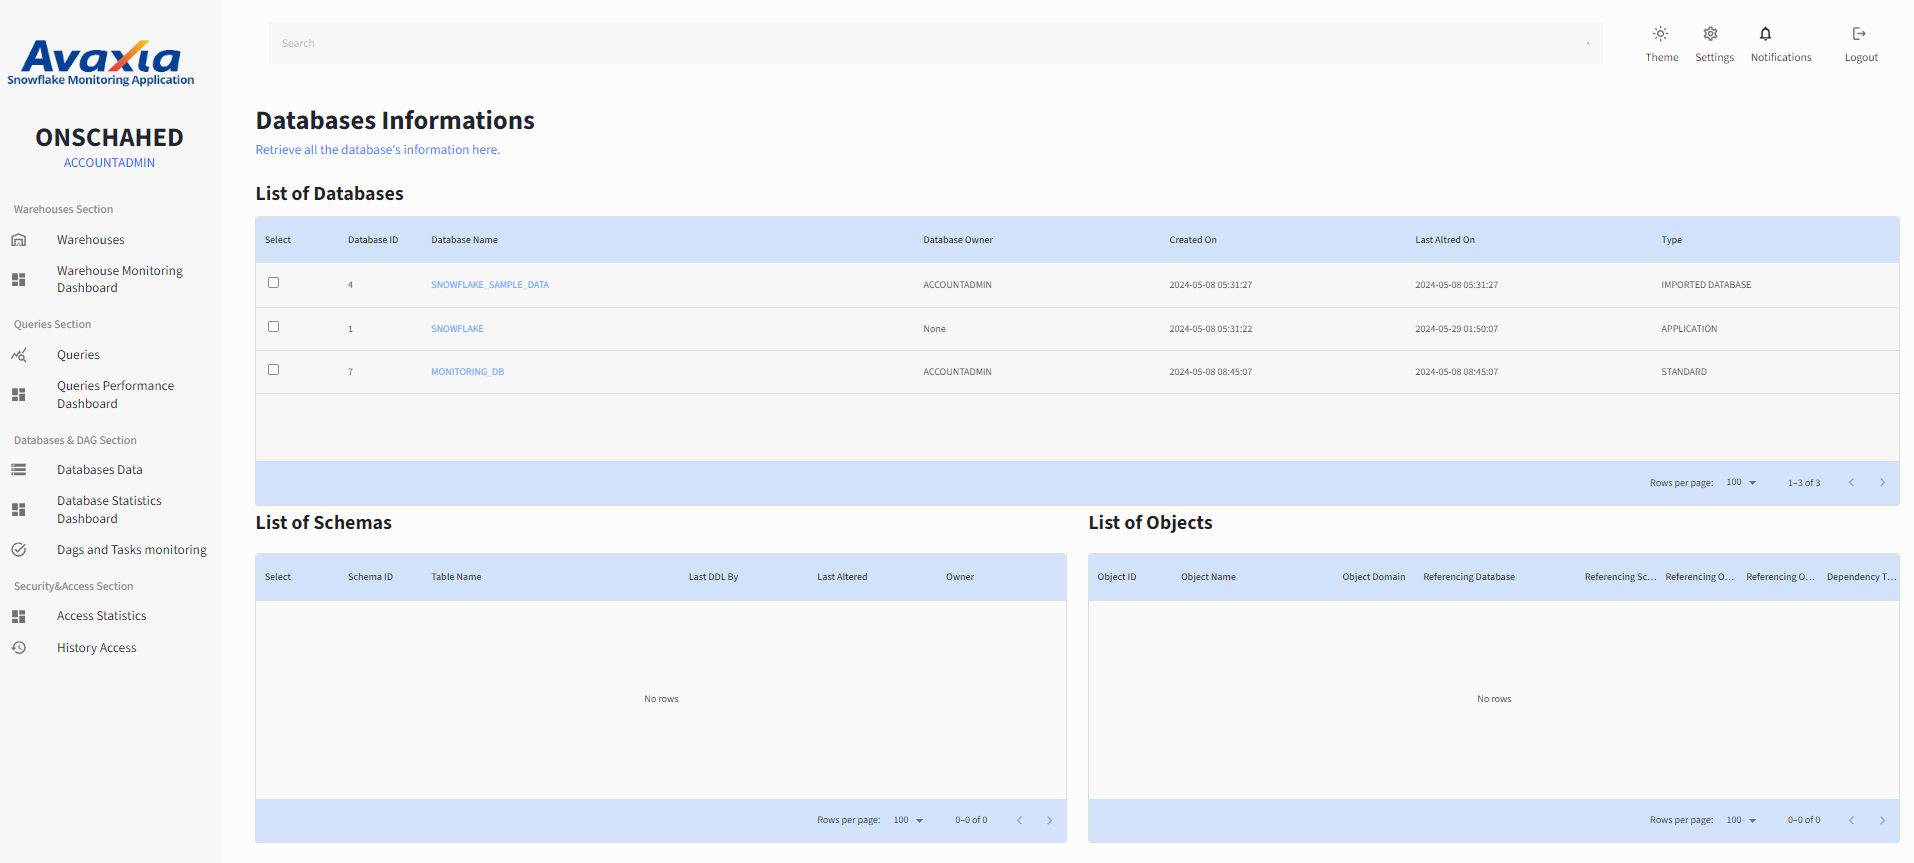
\includegraphics[width =1\linewidth]{img/captures/database/1.png}
            \caption{La liste des bases de données}
                \label{fig:dblist}
            \end{figure}
            \par La section "List of Databases" affiche les détails des différentes bases de données, y compris leur ID, leur nom, leur propriétaire et leurs dates de création et de dernière modification.\\ 
            Une fois l'utilisateur selectionne une base de données, la liste des schémas s'affiche comme l'indique la figure \textbf{\ref{fig:schemas}} suivante:
                \begin{figure}[H]
                \centering
                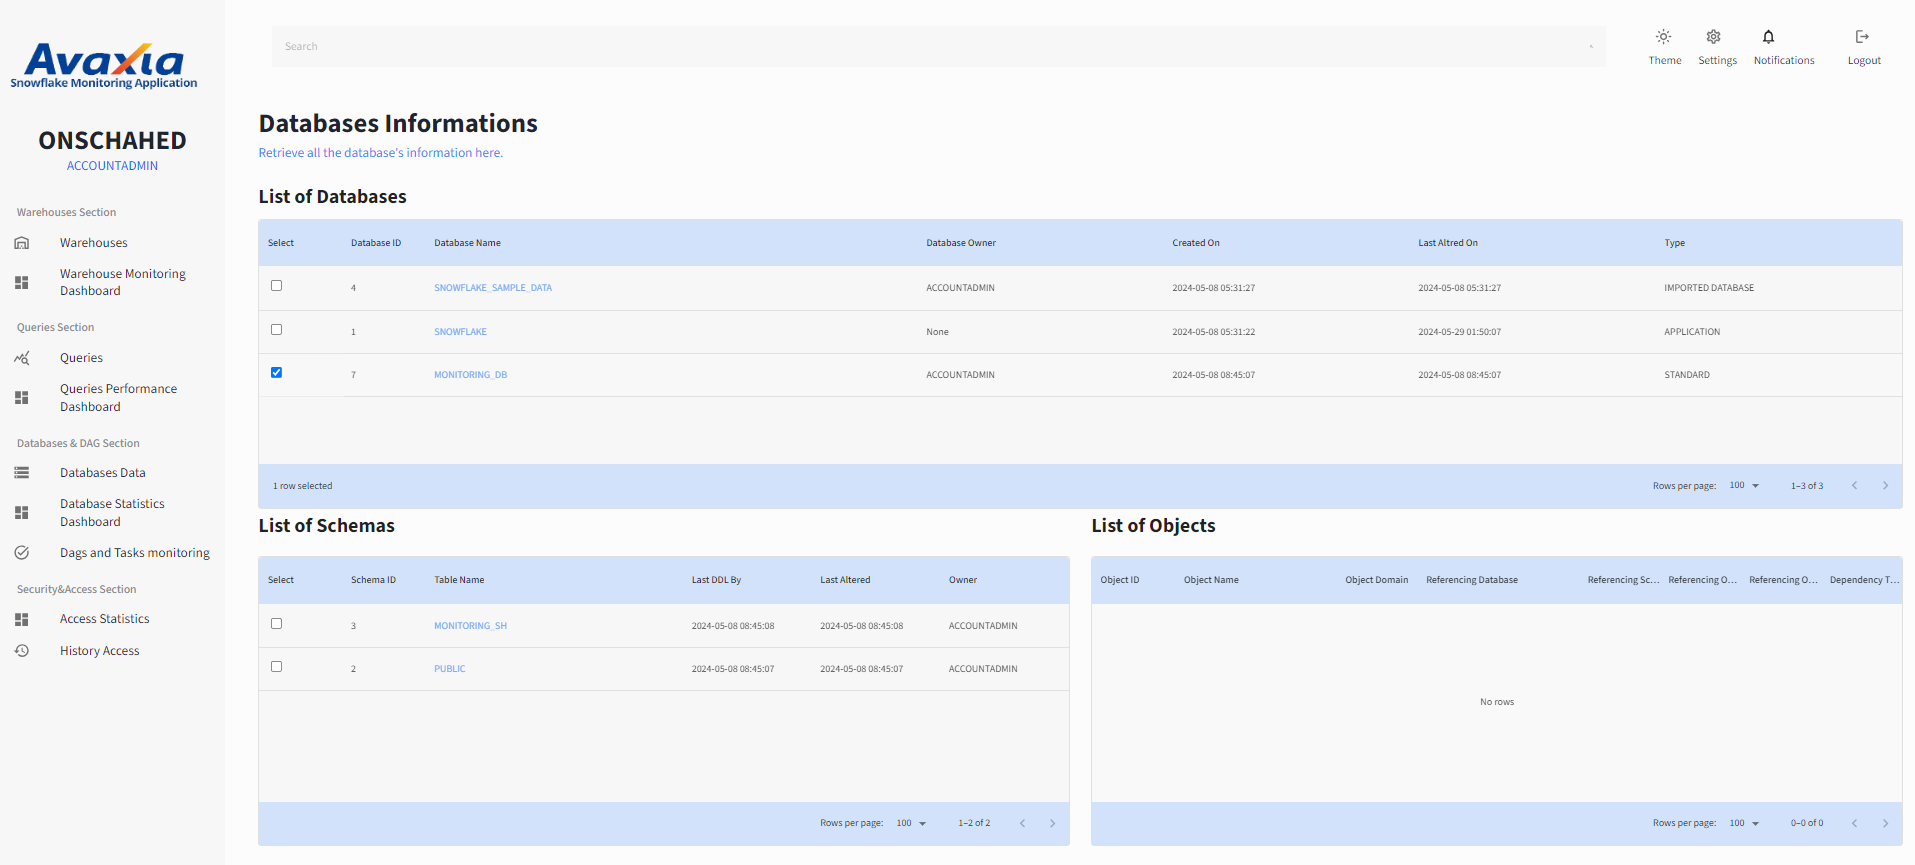
\includegraphics[width =1\linewidth]{img/captures/database/2.png}
                \caption{Liste des schémas de base de données}
                    \label{fig:schemas}
                \end{figure}

             Ensuite, pour que nous puissons lister les objets présents et créées dans cette base de données, l'utilisateur selectionne le schéma appriori pour lister ces objets.
            \par La figure \textbf{\ref{fig:objects}} illustre cette action :
            \begin{figure}[H]
                \centering
                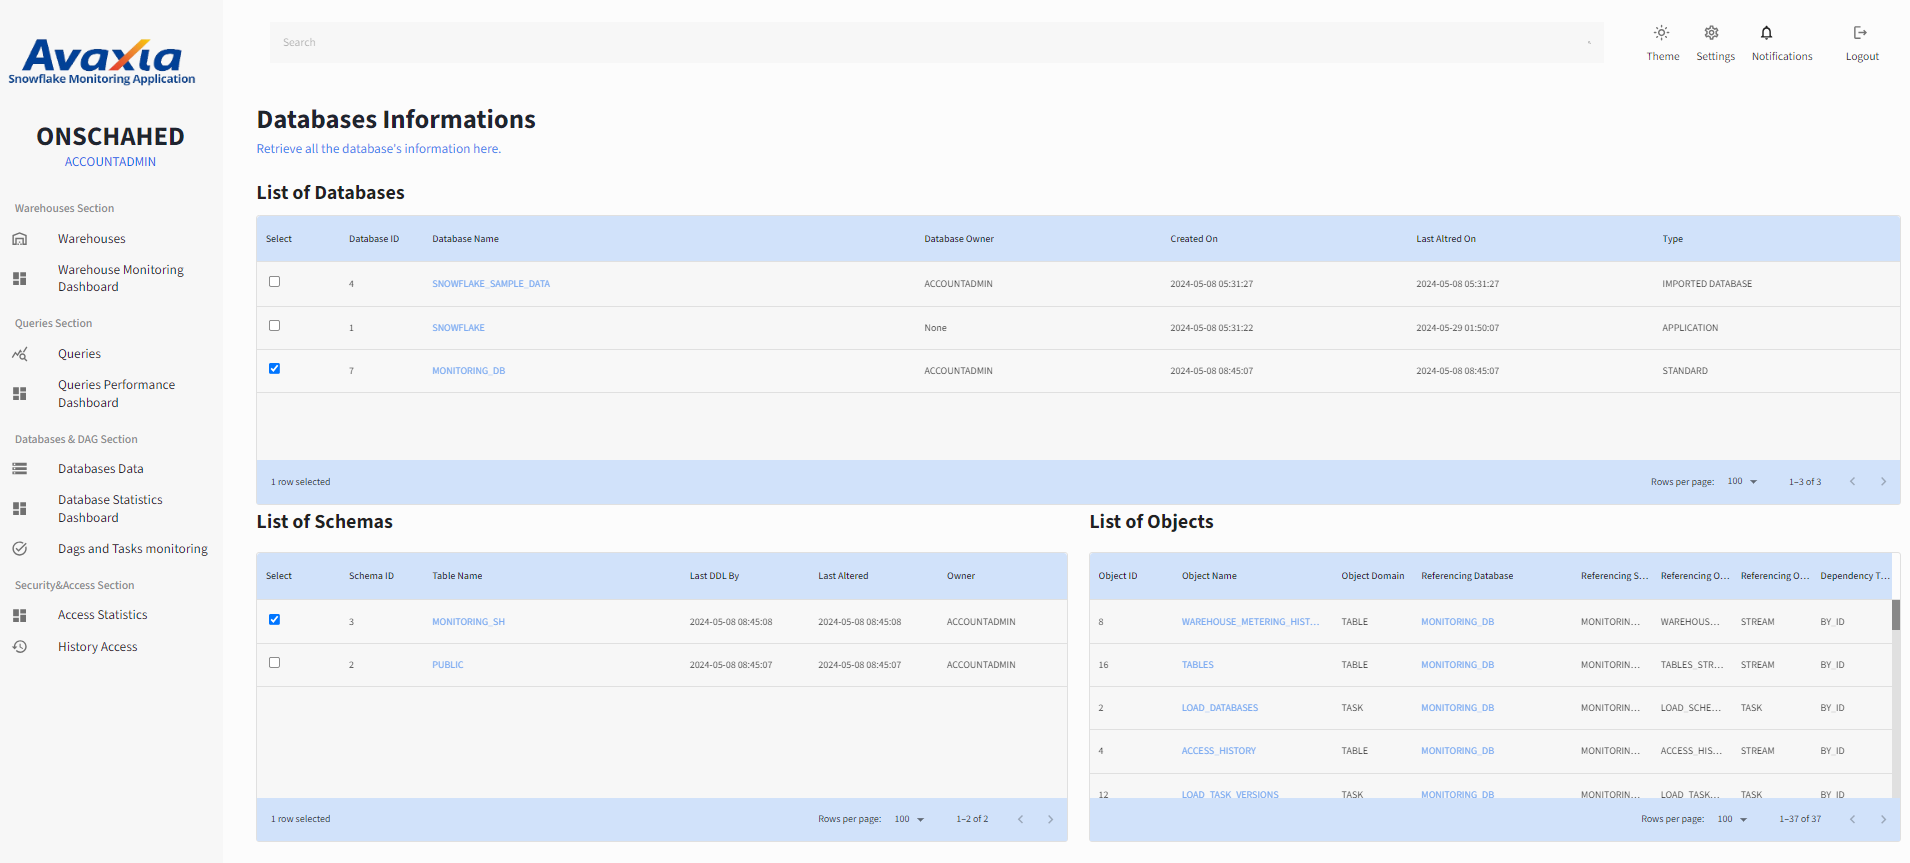
\includegraphics[width =1\linewidth]{img/captures/database/3.png}
                \caption{Liste des objets dans la base de données}
                    \label{fig:objects}
                \end{figure}
            \par Ces informations permettent aux administrateurs de l'application de surveiller et de gérer son compte Snowflake, en ayant une vue d'ensemble des bases de données, des schémas et des objets utilisés dans le système de surveillance.
             \item \textbf{Tableaux de bord du surveillance des bases de données :}
             \par La figure \textbf{\ref{fig:database}} représente le tableau de bord du surveillance des bases de données:
             \begin{figure}[H]
                \centering
                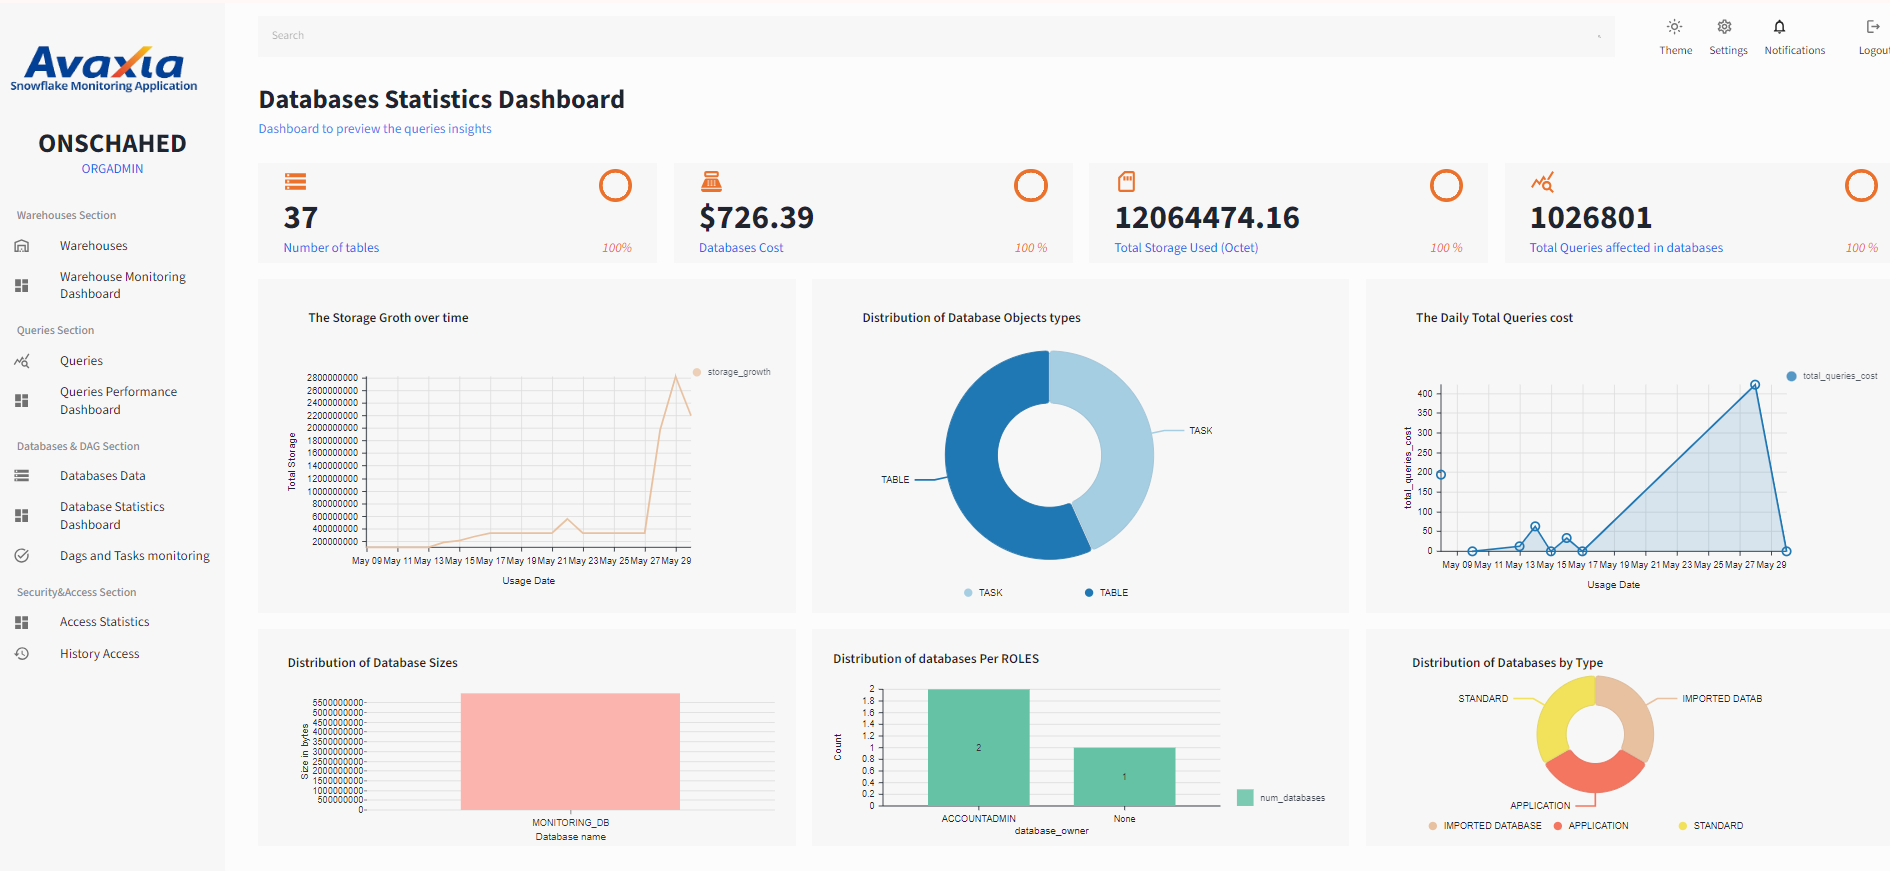
\includegraphics[width =1\linewidth]{img/captures/database/database_dash.png}
                \caption{Tableaux de bord du surveillance des bases de données}
                    \label{fig:database}
                \end{figure}
                \par Cette interface de tableau de bord des statistiques des bases de données fournit une vue d'ensemble complète des principales métriques liées à l'utilisation et à la gestion des données dans l'environnement Snowflake. 
                Elle présente des indicateurs clés tels que le nombre de tables, le coût total des bases de données, le stockage total utilisé et le nombre total de requêtes affectées.
                Les graphiques détaillés complètent ces informations en montrant l'évolution de l'utilisation du stockage, la répartition des types d'objets de base de données, la distribution des bases de données par rôle et par type, ainsi que l'évolution du coût quotidien des requêtes. \\ 
                
\end{itemize}
\par Ce microservice  offre aux administrateurs un outil complet et puissant pour surveiller les performances des bases de données, identifier les tendances clés et prendre des décisions éclairées afin d'optimiser l'utilisation et la gestion des coûts de leurs comptes.
\subsection{Micro-service << Access\_Statistics >>}
\par Le micro-service << Access\_Statistics >>  est le service chargé de la surveillance des accées aux comptes Snowflake.
\begin{itemize}
    \item \textbf{La liste des APIs:}
        \par La liste des APIs présents dans ce micro-service, documentée par Swagger, sont representés par la figure \textbf{\ref{fig:apiAccess}} suivante:
        \begin{figure}[H]
            \centering
            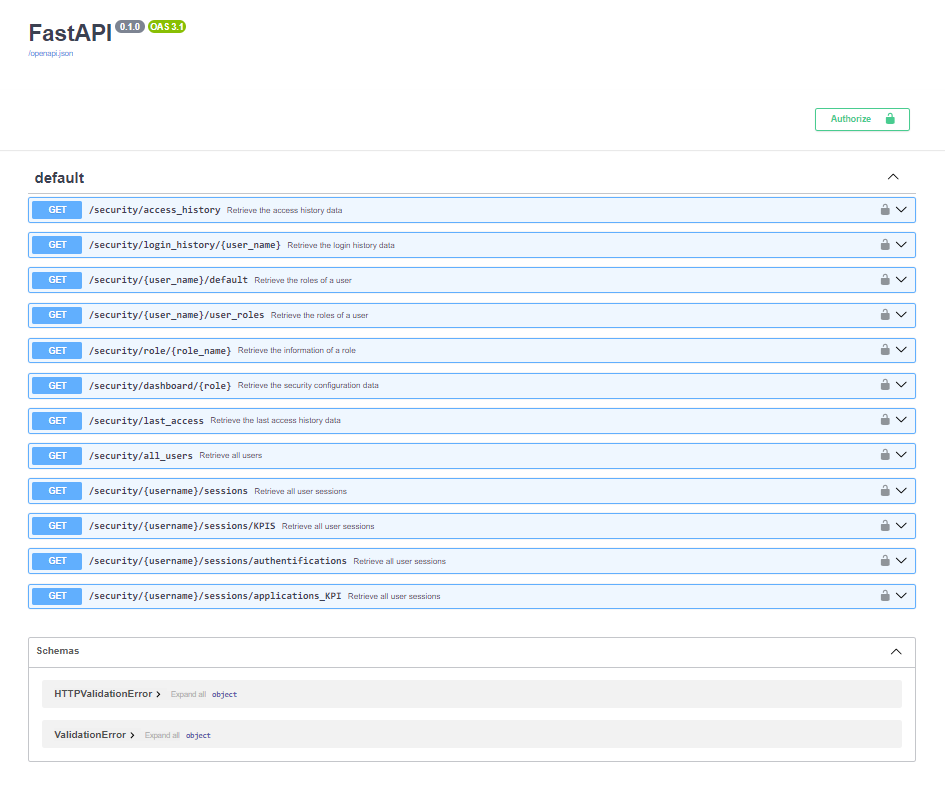
\includegraphics[width =1\linewidth]{img/captures/access_apis.PNG}
            \caption{Liste des APIs du microservice << Access\_Statistics >> }
                \label{fig:apiAccess}
        \end{figure}

        \item \textbf{L'historique des accés de l'utilisateur ONS CHAHED :}
        \par L'interface de l'historique d'accés est representée par la figure \textbf{\ref{fig:accesslist}} suivante:
        \begin{figure}[H]
            \centering
            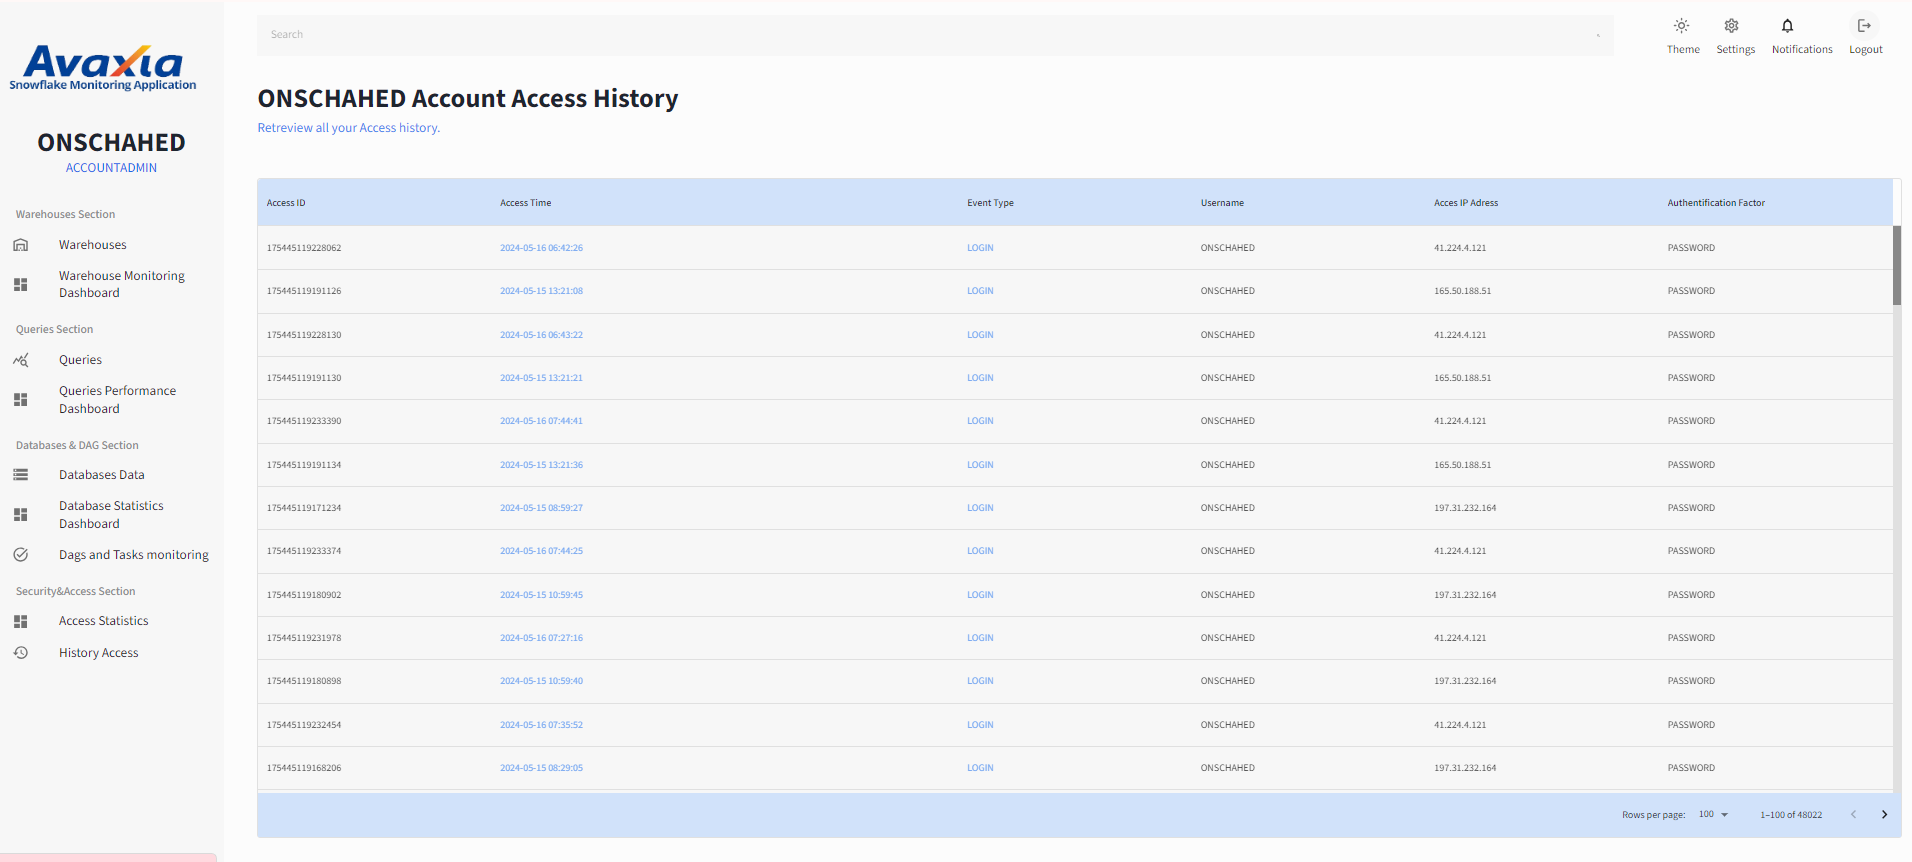
\includegraphics[width =1\linewidth,height =14cm]{img/captures/user/history.png}
            \caption{Historique des accées}
                \label{fig:accesslist}
            \end{figure}
            \par Cette interface d'historique des accès fournit une traçabilité complète des activités dans l'environnement Snowflake. 
            Elle enregistre de manière détaillée chaque événement d'accès, capturant des informations clés telles que l'identité de l'utilisateur, l'heure d'accès et les méthodes d'authentification utilisées. \\
            Ce journal d'activité exhaustif représente un outil de gouvernance et de surveillance essentiel pour les administrateurs. 
            Il leur permet de suivre les mouvements des différents acteurs au sein du système, de détecter d'éventuelles activités suspectes et d'assurer la sécurité globale de l'infrastructure.
            \item \textbf{Tableaux de bord du surveillance des accéess des utilisateurs:}
             \par Les figures \textbf{\ref{fig:acess1}} et \textbf{\ref{fig:acess2}} représentent les tableaux de bord du surveillance des accés de l'utilisateur <<ONS CHAHED>> et l'utilisateur système <<Snowflake>>:
             \begin{figure}[H]
                \centering
                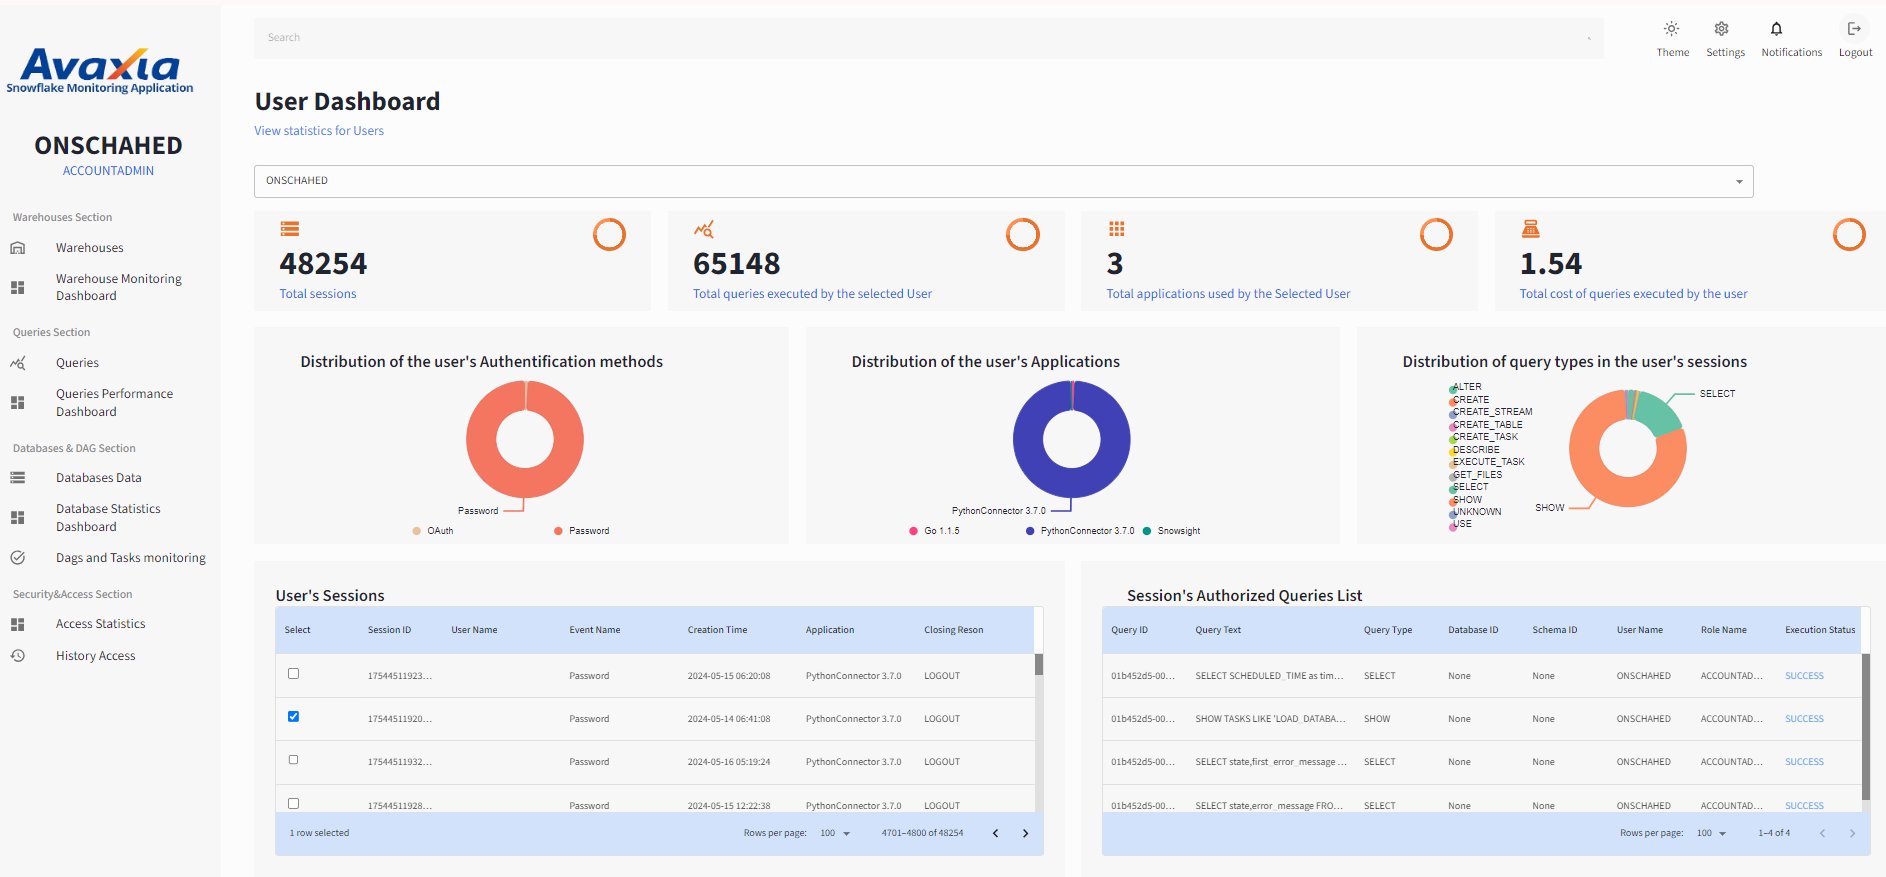
\includegraphics[width =1\linewidth]{img/captures/user/1.png}
                \caption{Tableau de bord du surveillance des accés de l'utilisateur <<ONS CHAHED>>}
                    \label{fig:acess1}
                \end{figure}
                \begin{figure}[H]
                    \centering
                    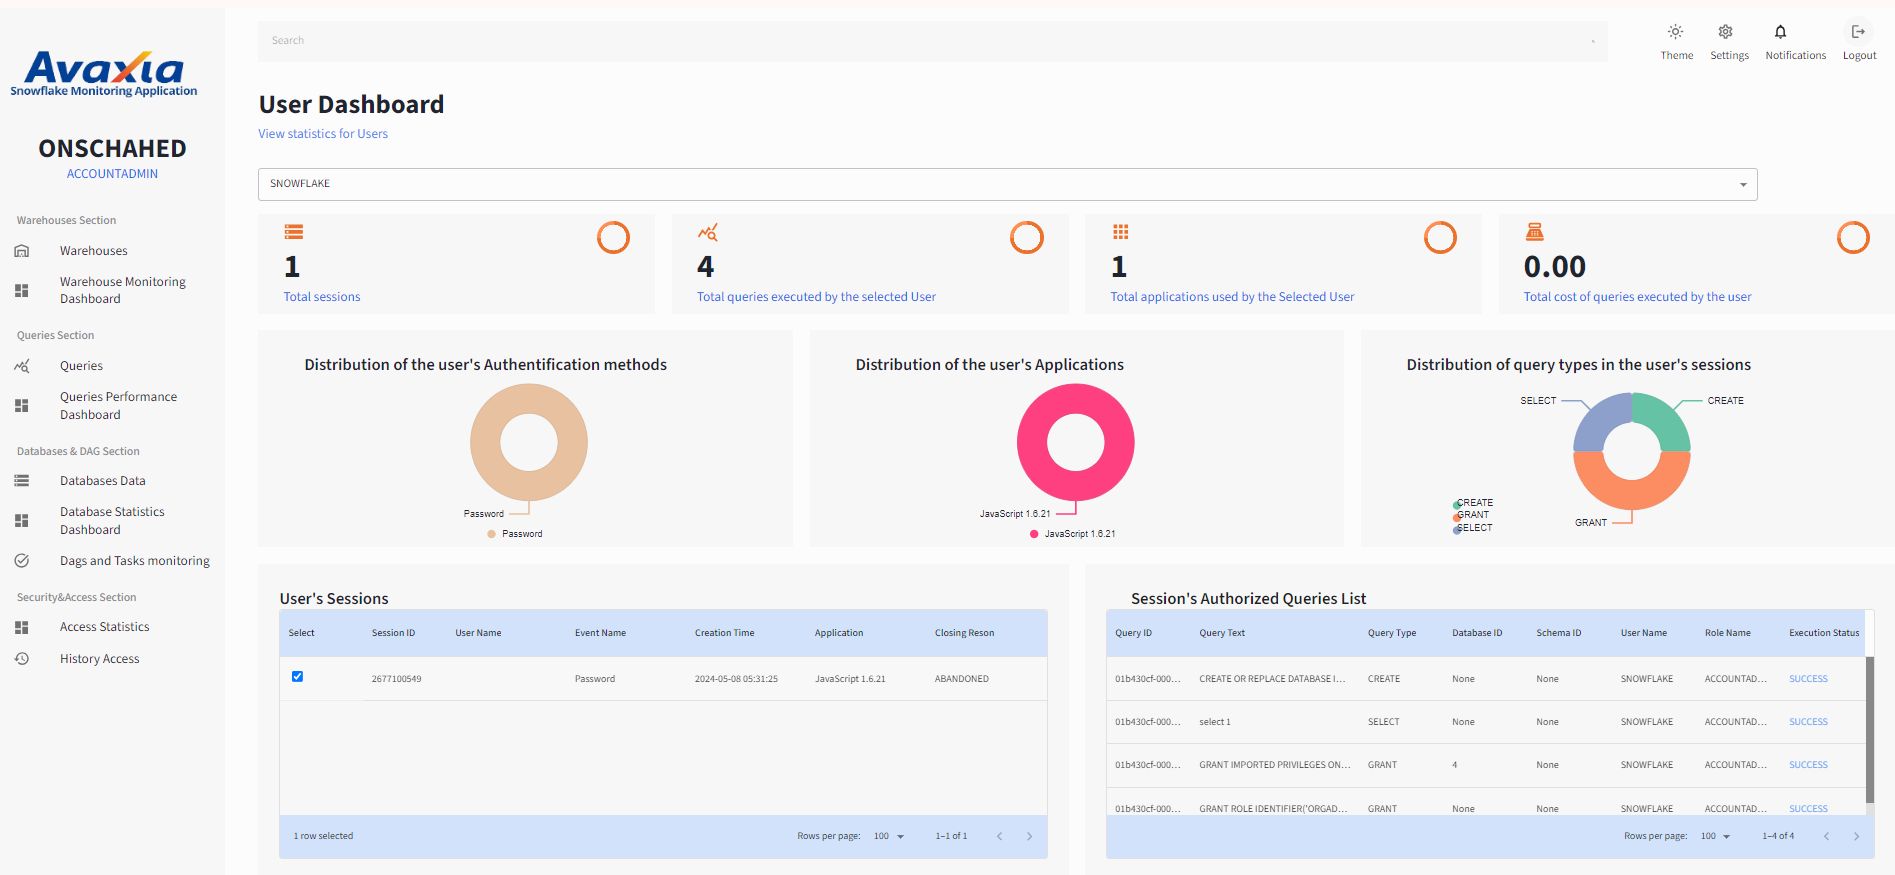
\includegraphics[width =1\linewidth]{img/captures/user/2.png}
                    \caption{Tableau de bord du surveillance des accés de l'utilisateur <<SNOWFLAKE>>}
                        \label{fig:acess2}
                    \end{figure}
                \par Ces tableaux de bord offrent une visibilité complète sur l'activité des différents utilisateurs au sein de l'environnement Snowflake. Ils permettent de suivre des indicateurs clés tels que le nombre de sessions, de requêtes exécutées, d'applications utilisées et les coûts associés. Ces données quantitatives fournissent une image détaillée de l'utilisation du système par chaque utilisateur.
                \\ L'historique détaillé des sessions et des requêtes autorisées complète ce tableau, donnant aux administrateurs une traçabilité exhaustive des actions entreprises par chaque utilisateur. Cet outil de suivi leur permet de détecter les éventuelles anomalies et de s'assurer du respect des politiques d'accès.
                Ils fournissent aux équipes opérationnelles les informations nécessaires pour prendre des décisions éclairées en matière de sécurité, de contrôle d'accès et d'utilisation des ressources.
\end{itemize}
\par Ce microservice de surveillance des accès est bien plus qu'un simple registre. C'est un levier puissant pour les équipes en charge de la gouvernance et de l'exploitation des systèmes de données, leur permettant de prendre des décisions éclairées et de maintenir la fiabilité et la résilience de l'environnement Snowflake dans le temps.
\subsection{Micro-service << DAG\_Monitoring >>}
\par C'est le service responsable du suivi et de la surveillance en temps réelle des flux de tâches (<<DAG>>) exécutées et programmées dans Snowflake. 
\par Dans cette section, nous allons surveiller l'éxécution d'un ensemble des tâches en temps réelle. 
\\ Ces tâches là sont déjà créées dans notre compte Snowflake de test, la figure \textbf{\ref{fig:show}} illustre la liste des tâches dont nous allons monitorer dans snowflake, qui apparaître en exécutant la command << Show TASKS >>:
    \begin{figure}[H]
        \centering
        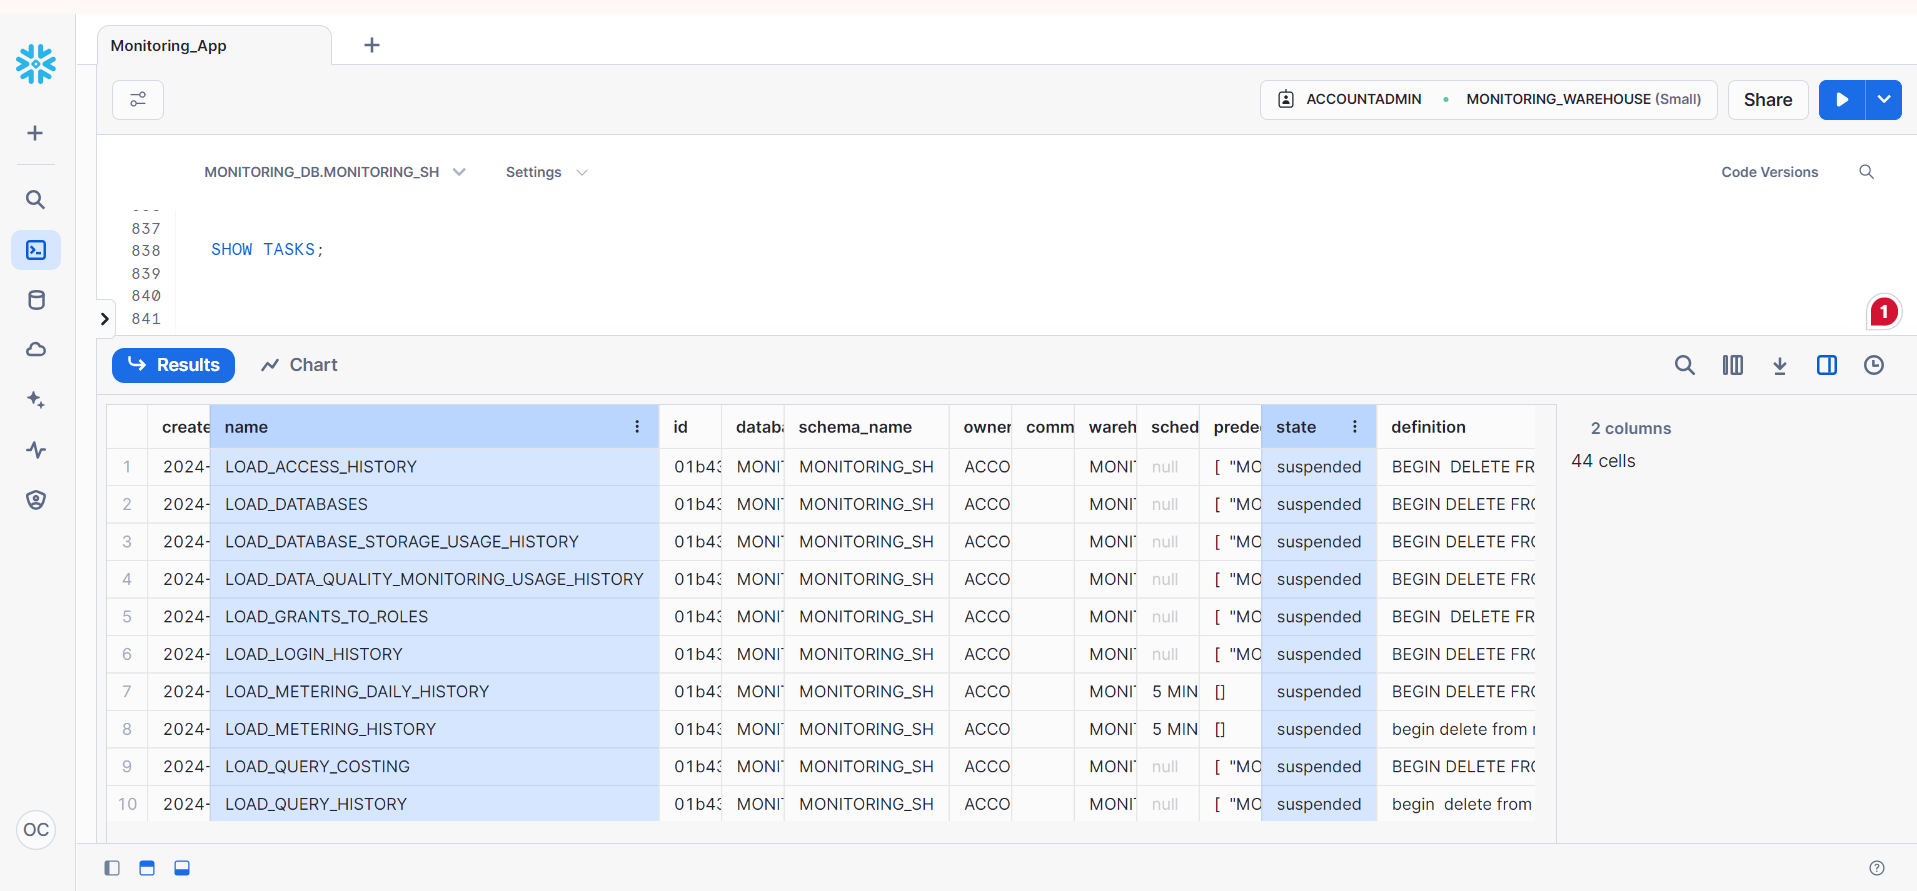
\includegraphics[width =1\linewidth]{img/captures/dag/show.PNG}
        \caption{Résultat du command <<Show tasks>> }
        \label{fig:show}
    \end{figure}
\par Simultanément, dans notre application, les tâches sont illustrés par la figure \textbf{\ref{fig:sus}} dans le même état <<SUSPENDED>> que dans snowflake:
    \begin{figure}[H]
        \centering
        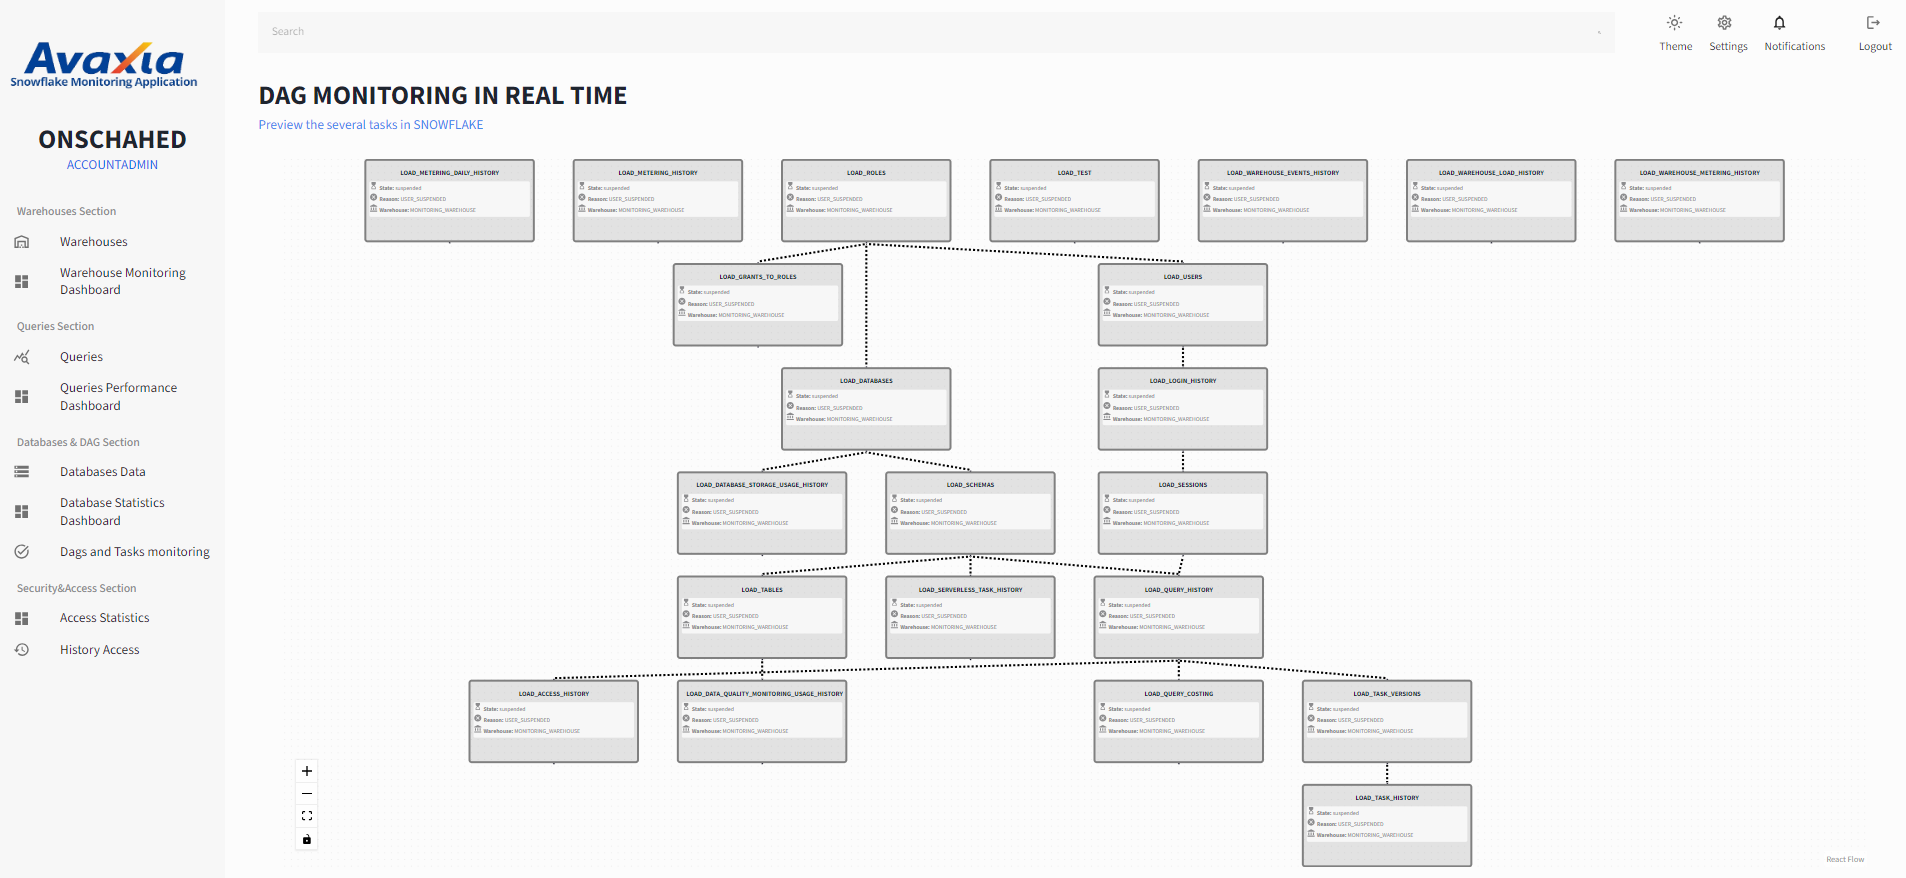
\includegraphics[width =1\linewidth]{img/captures/dag/1/ok/0.png}
        \caption{Etape 0 : état initial du DAG}
        \label{fig:sus}
    \end{figure}
\par Une fois nous résumons l'exécution des tâches dans snowflake avec les commandes de la figure \textbf{\ref{fig:resume}} :
\begin{figure}[H]
    \centering
    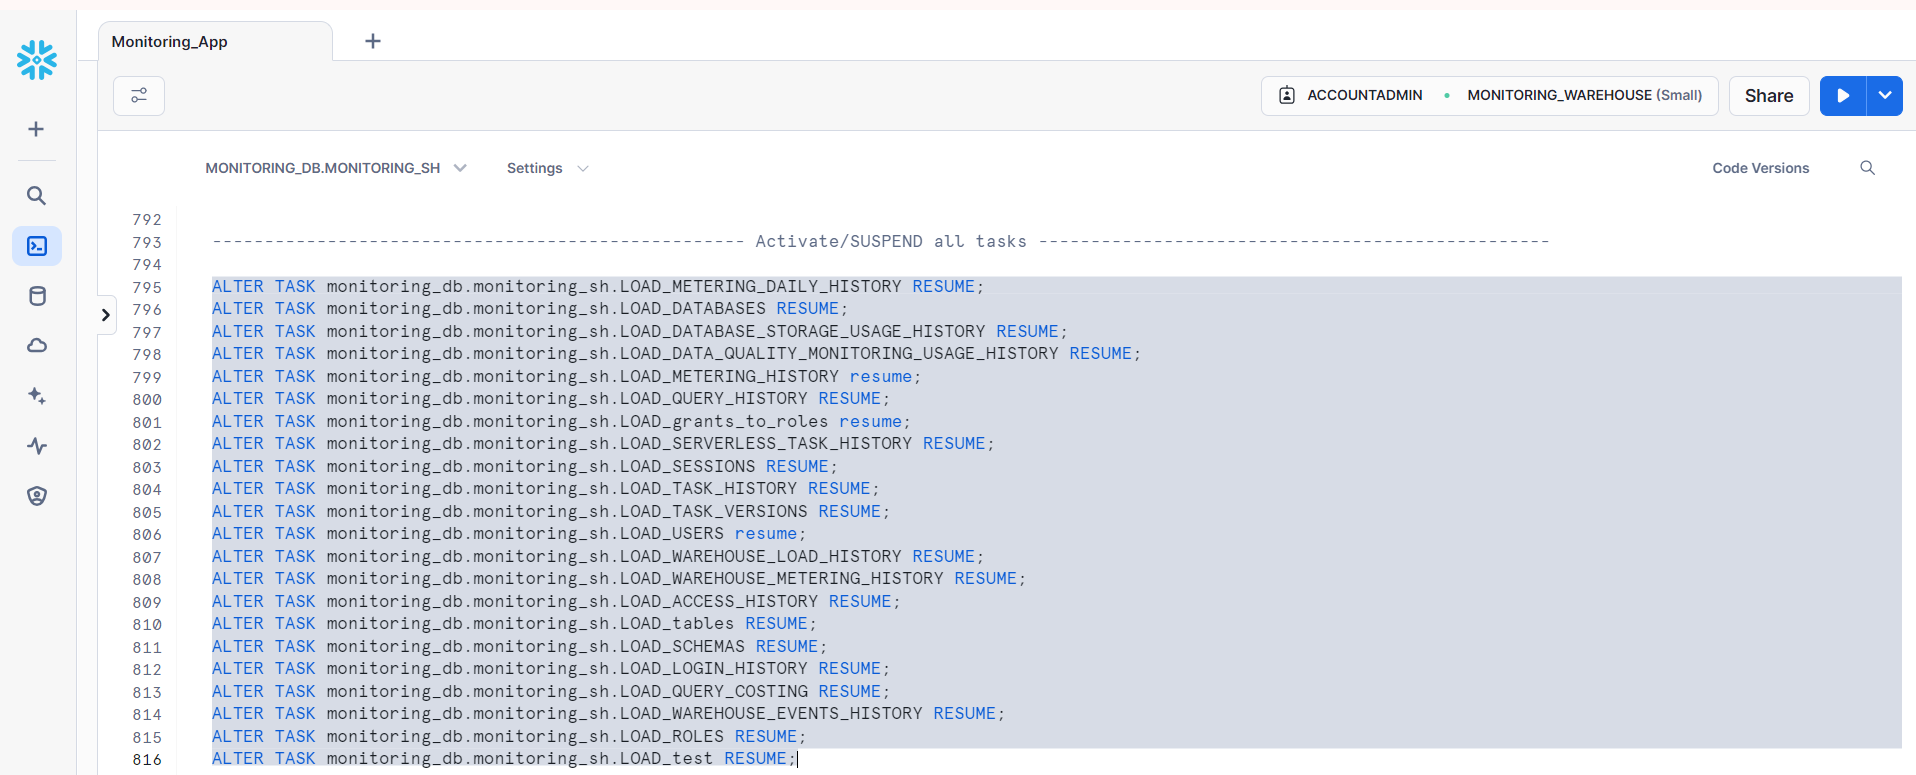
\includegraphics[width =1\linewidth]{img/captures/dag/resume.png}
    \caption{Lancement de l'éxécution des tâches}
    \label{fig:resume}
\end{figure}
\par La visualisation du DAG commence à s'animer comme l'indique la figure \textbf{\ref{fig:sus}} suivante telque :
\begin{itemize}
    \item Les tâches qui représentent les racines de DAG doivent être toujours programmées pour qu'elles se lancent d'une façon séquentielle ;
    \item Les sous-tâches suitent l'exécution de la tâche racine ;
    \item L'état courant des sous tâches lorsque la racine est programmée préserve le dernier état aprés la derniére éxecution.
\end{itemize}
\begin{figure}[H]
    \centering
    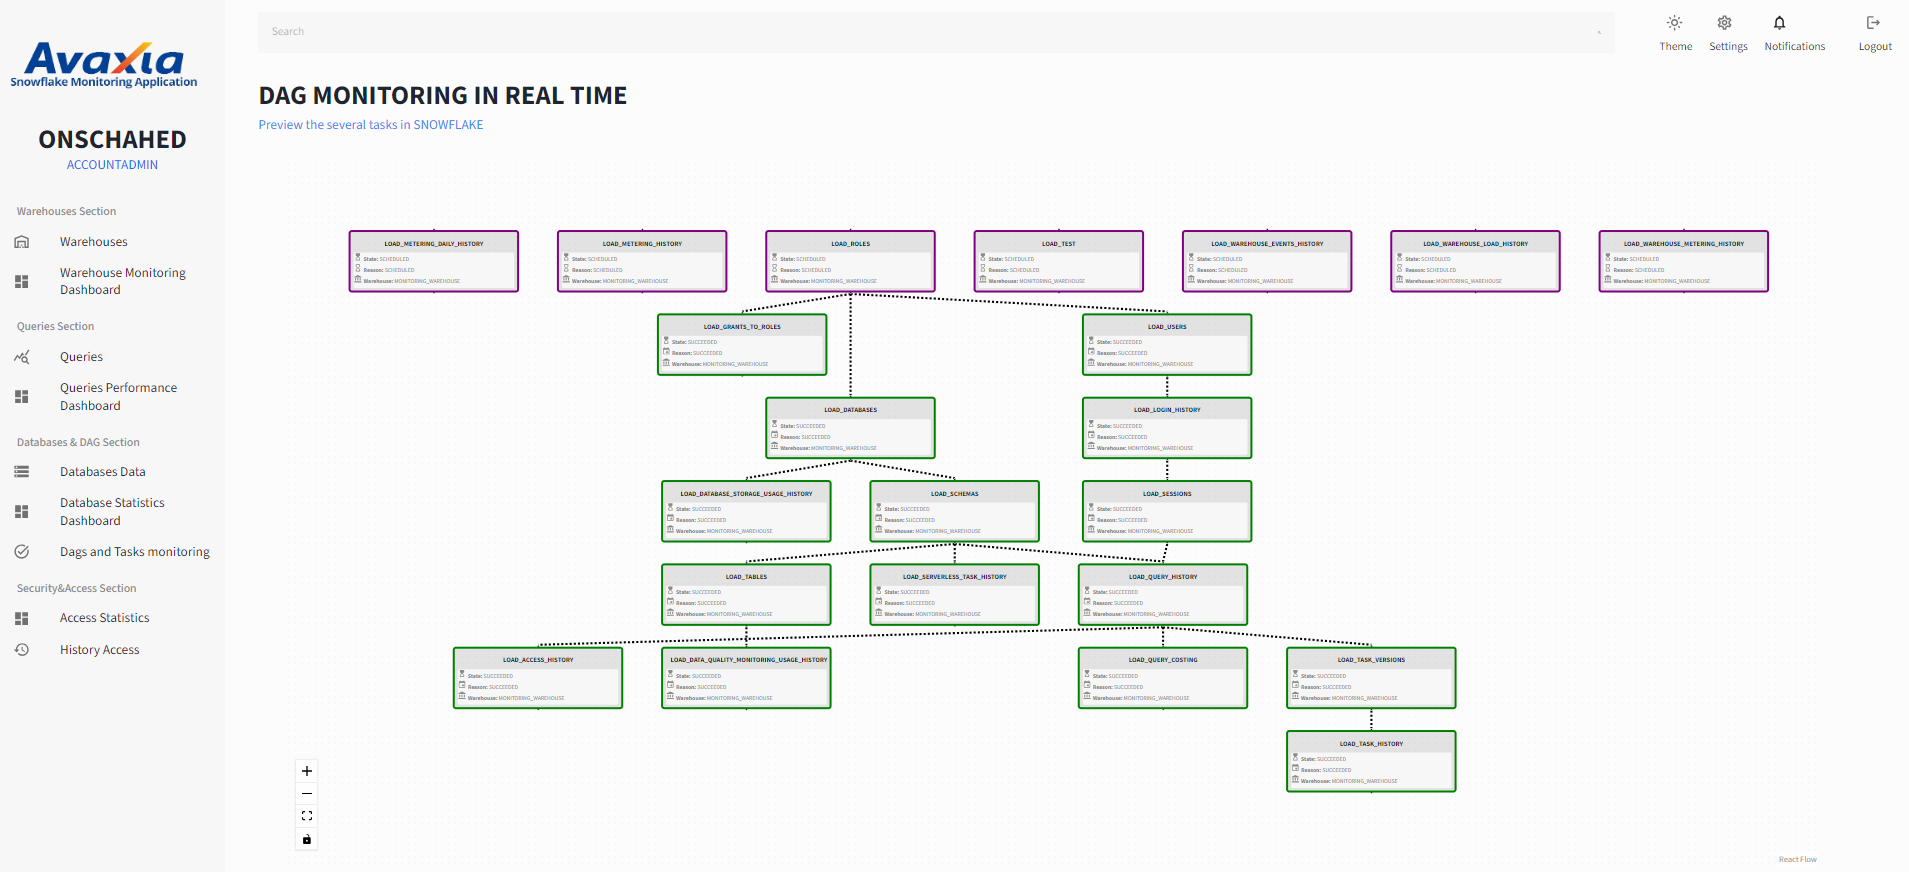
\includegraphics[width =1\linewidth]{img/captures/dag/scheduled.png}
    \caption{Etape 1 : Lancement des têches}
    \label{fig:sus}
\end{figure}
\par Maintenant, nous allons superviser le DAG du tâche \textbf{<<Load roles>>}. \\
Initialement, cette tâche est \textbf{programmée} chaque 5 minutes, elle est colorée en \textbf{<< violet >>} et tous ces sous-tâches sont colorées en \textbf{<< vert >>} pour indiquer que leurs dernier état était un succés. \\
Aprés 5 minutes, l'état de la tâche racine se modifie de \textbf{programée} (<<Scheduled>> ) vers \textbf{en exécution} (<<Executing>>) et sa couleur devenue \textbf{<< bleu>> }. \\
Parallélement, les sous-tâches du premier niveau, \textbf{<<Load\_grant\_to\_roles>>}, \textbf{<<Load users>>} et \textbf{<<Load databases>>} deviennent \textbf{programmées} mais pour quelques instants car une fois la tâche supérieure compléte son éxécution ces tâches s'éxécutent directement.
La figure \textbf{\ref{fig:executing}} illustre ce qui précéde:
    \begin{figure}[H]
    \centering
    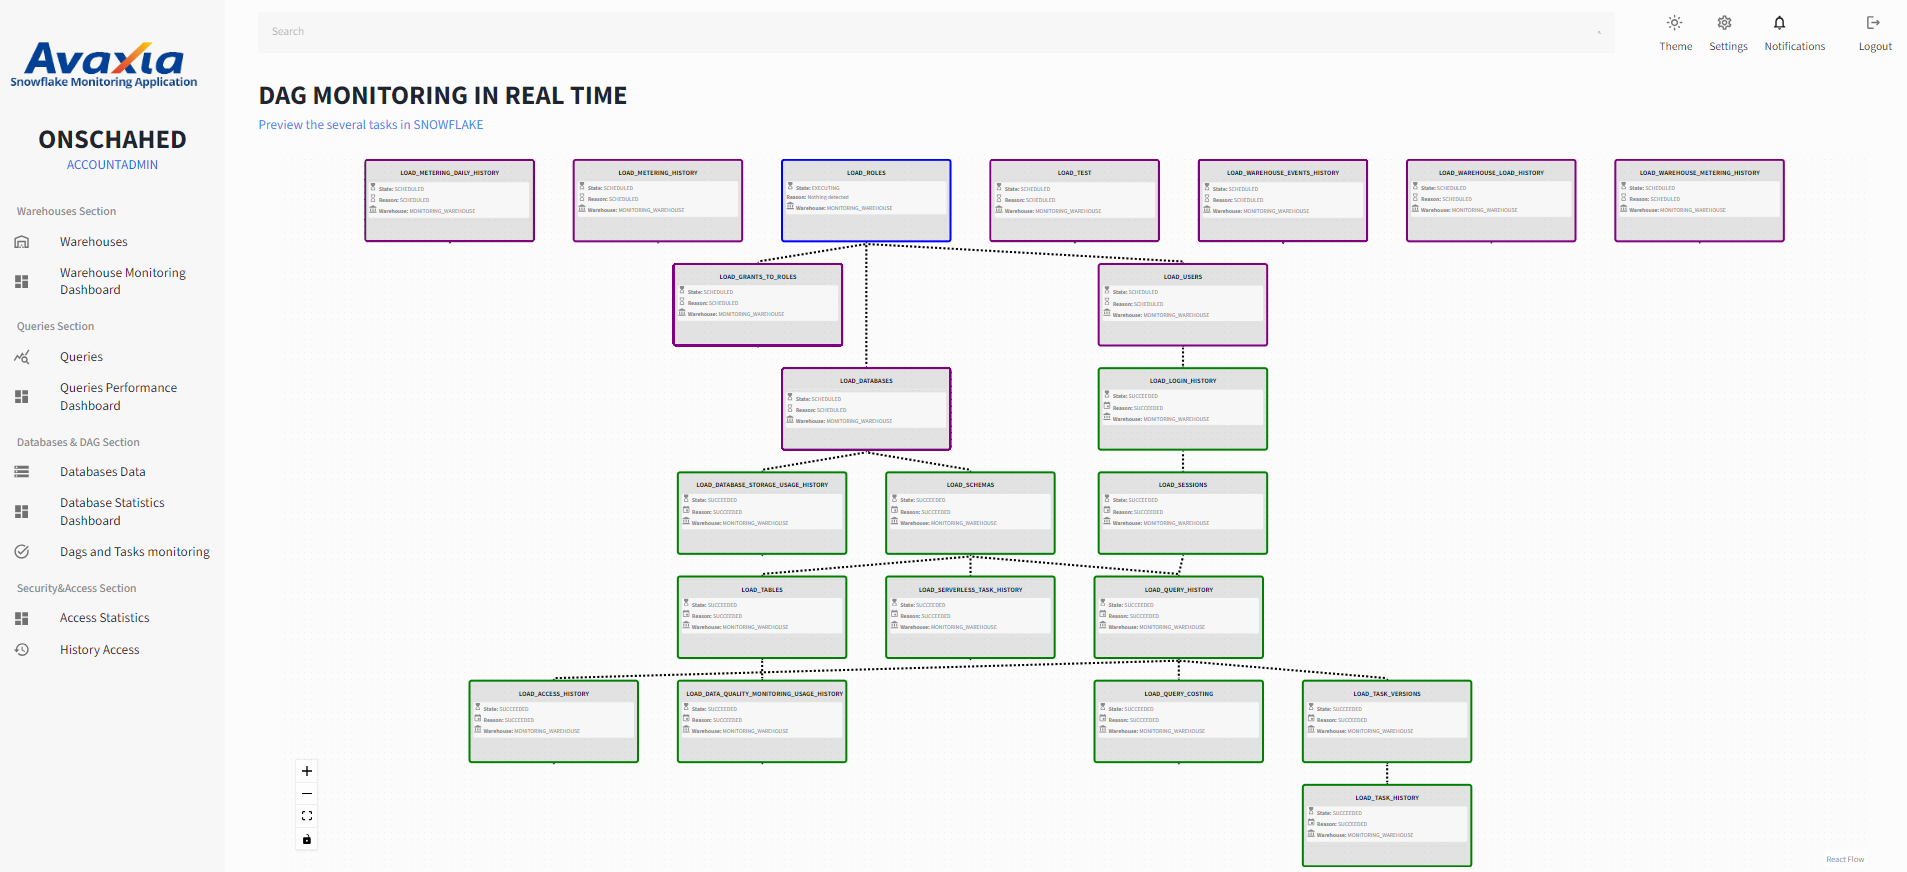
\includegraphics[width =1\linewidth]{img/captures/dag/final/1.png}
    \caption{Etape 3 : Execution de la racine}
    \label{fig:executing}
    \end{figure}
\par Une fois la tâche << Load roles >> est \textbf{éxecutée avec succés}, ses sous-tâches s'exécutent à leurs tour aussi comme l'indique la figure \textbf{\ref{fig:success}}
\begin{figure}[H]
    \centering
    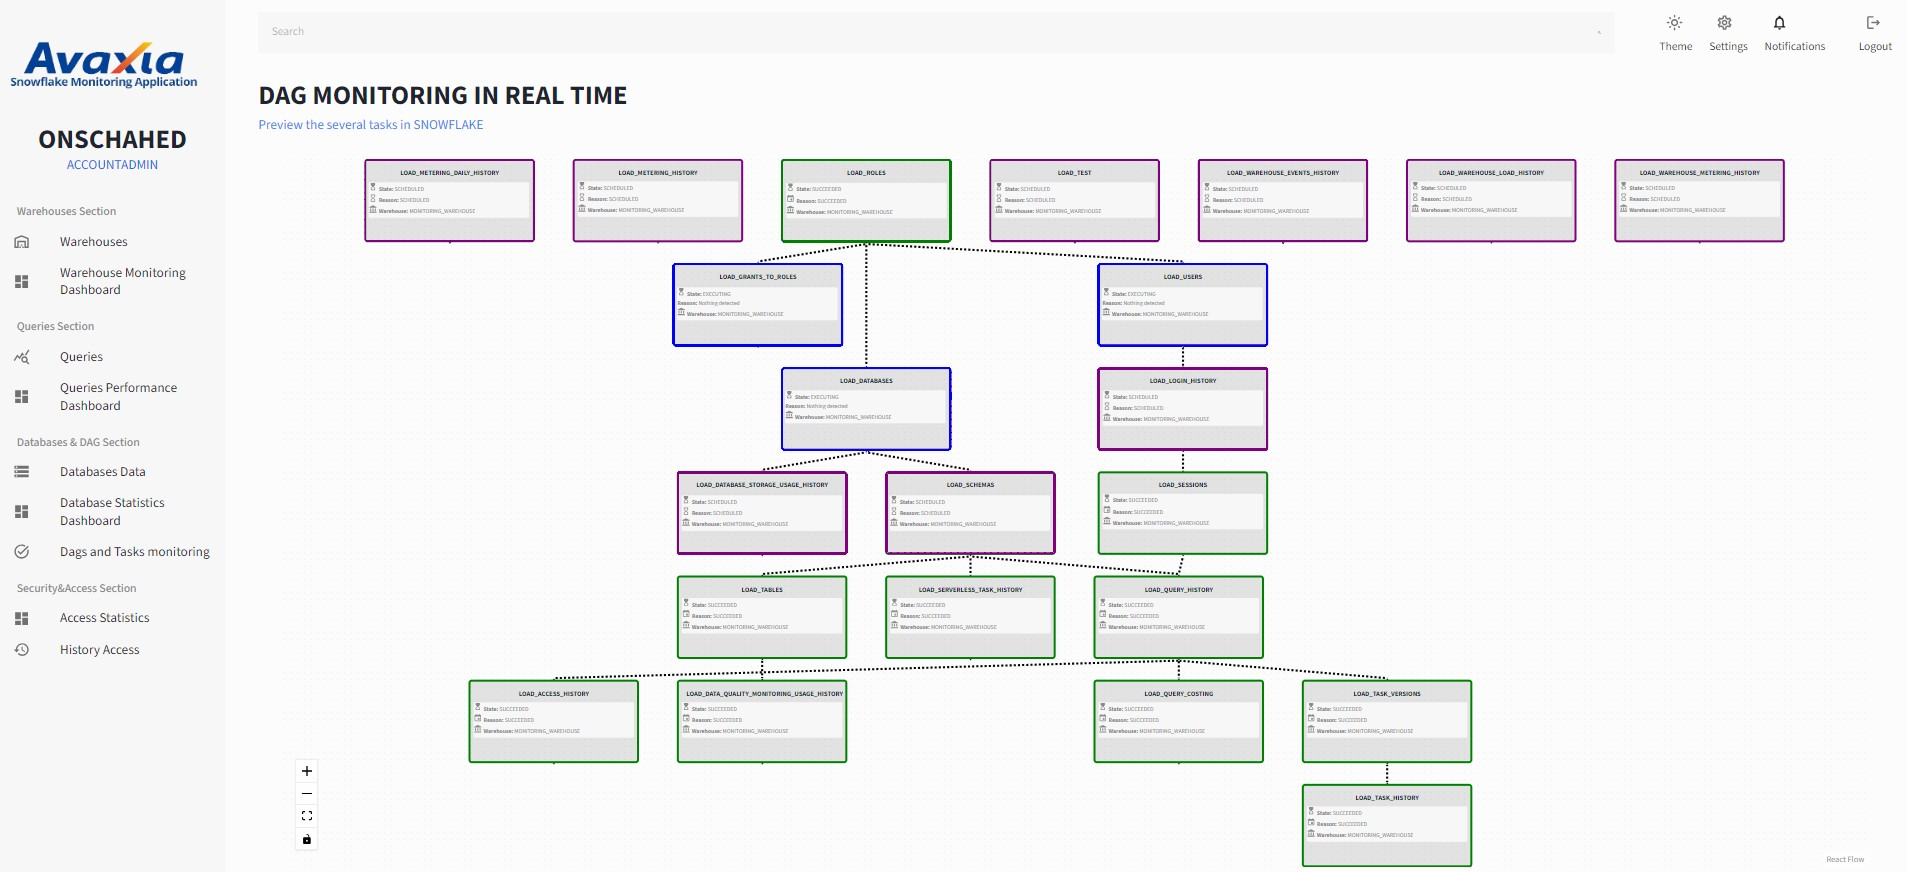
\includegraphics[width =1\linewidth]{img/captures/dag/final/2.jpg}
    \caption{Etape 4 : Exécution des sous-tâches de niveau I}
    \label{fig:success}
    \end{figure}

\par Ce cycle ce répete d'un niveau à un autre jusqu'à avoir un succés par tout dans le DAG comme l'indique la figure \textbf{\ref{fig:final}} suivante.\\
 À cet instant là, l'état du DAG revient à l'etape 1 du cycle si aucune malveillance est produite, sinon la tâche erronée va être colorée en \textbf{<<rouge>>}  et en affichant le message d'erreur (présent dans la figure \textbf{\ref{fig:error}}), ce qui le cas de la tâche \textbf{<<load test>>} dans la même figure. 
\begin{figure}[H]
    \centering
    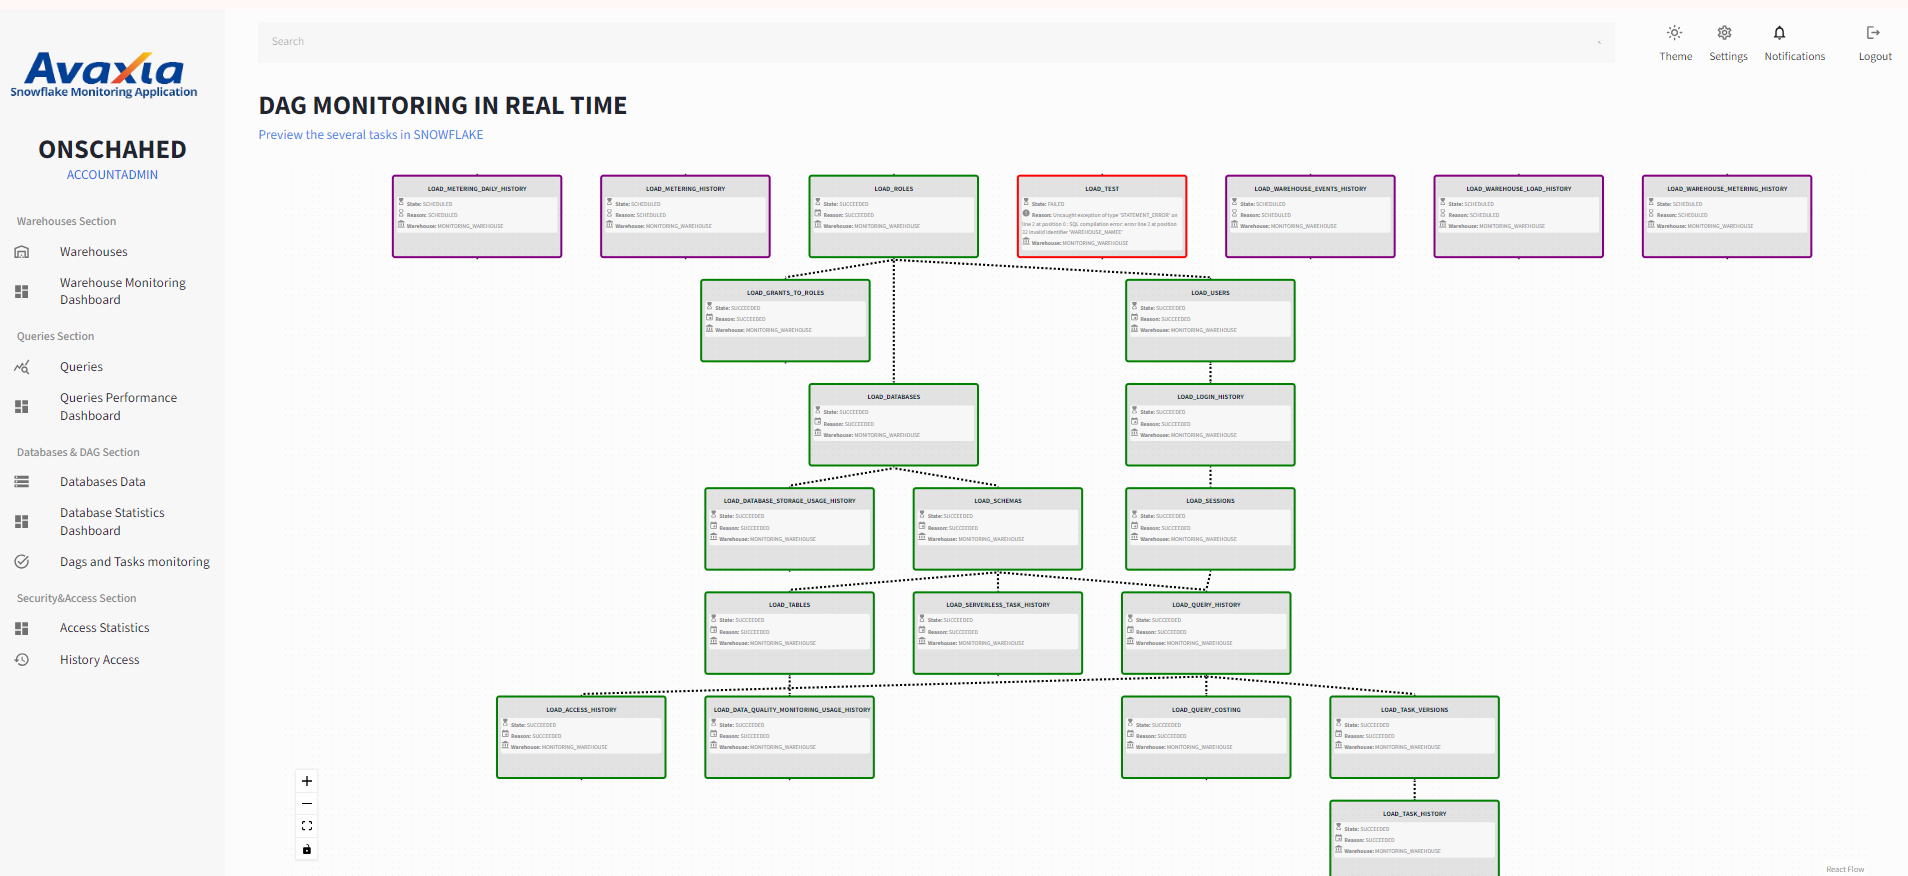
\includegraphics[width =1\linewidth]{img/captures/dag/final/failed.png}
    \caption{Etape 5 : Succes dans tous les branches du DAG <<Load Roles>>}
    \label{fig:final}
    \end{figure}
    \begin{figure}[H]
        \centering
        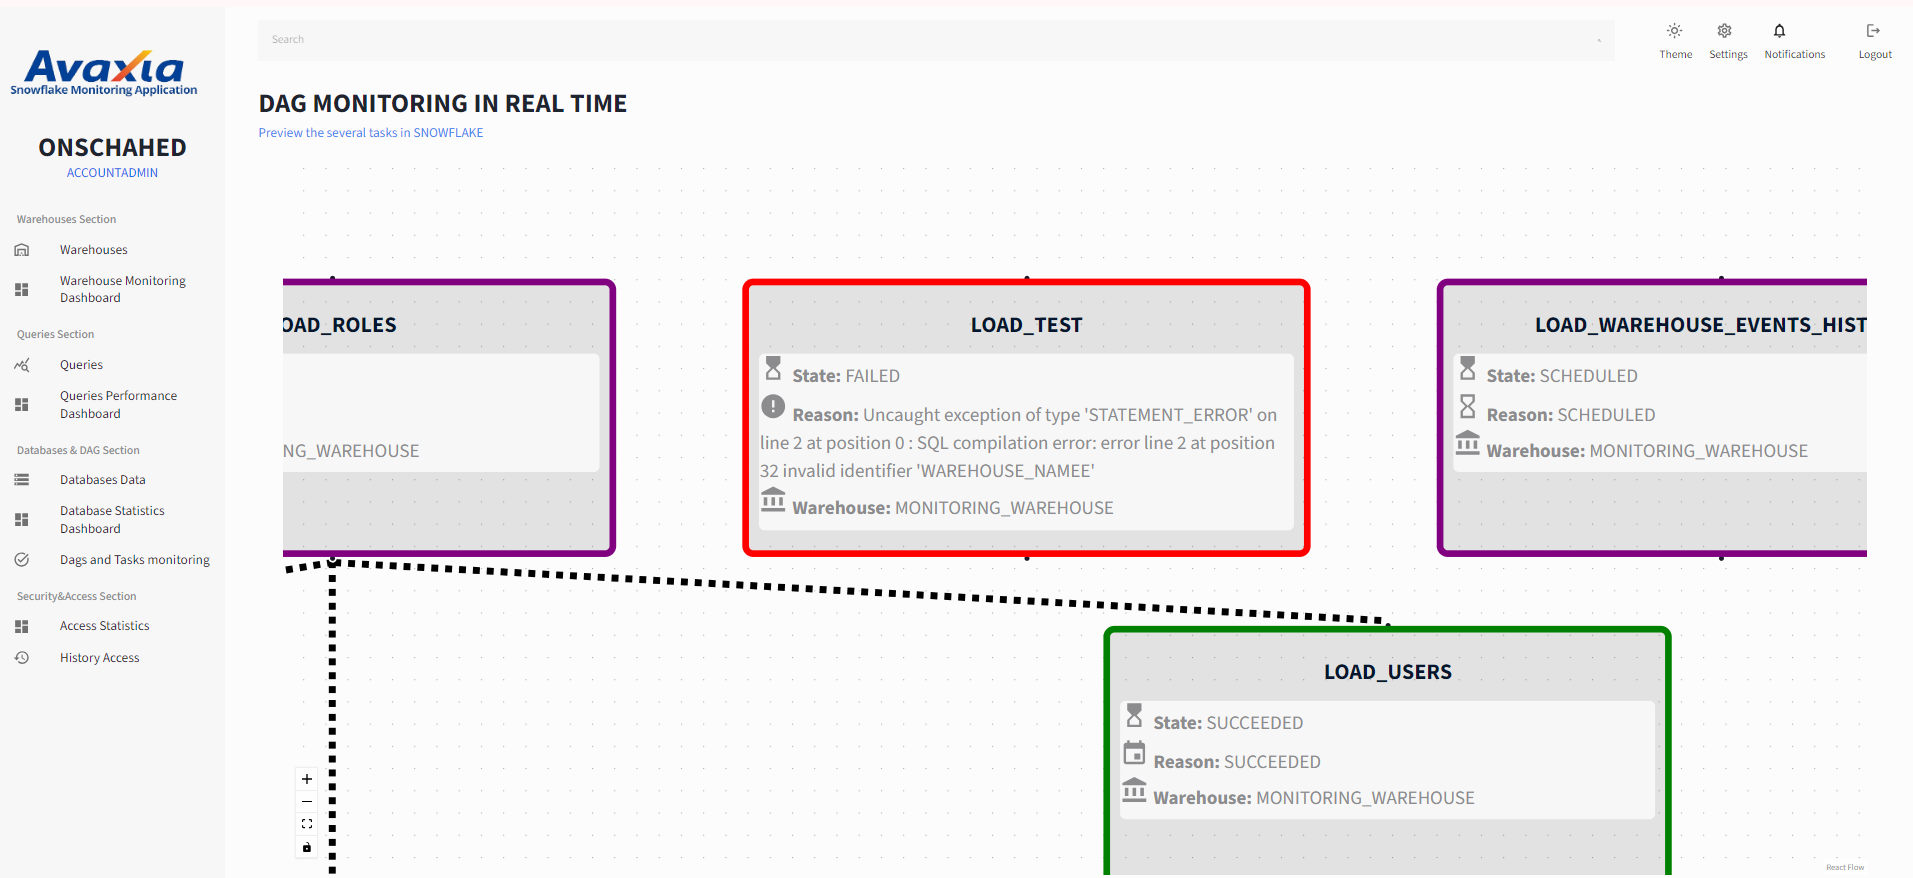
\includegraphics[width =1\linewidth]{img/captures/dag/final/reason.png}
        \caption{Message d'erreur de la tâche <<Load test>>}
        \label{fig:error}
        \end{figure}
\par Il faut noter que, si l'erreur d'une tâche persiste, Snowlfake va suspendu cette tâche pour ne pas affectée les tâches en relations avec elle. 
Bien évidement, si cette tâche erronée est présente dans une DAG, la tâche racine va être auto-suspendu directement ce qui va empécher l'execution de tout les autres sous-tâches \cite{auto}. 
\par la figure \textbf{\ref{fig:autosus}} montre l'auto-suspend de la tâche <<load test>> aprés exactement 10 tentative d'éssai (un paramêtre par défaut dans Sonwflake fixé à 10) qui ont donné des erreurs.
\begin{figure}[H]
    \centering
    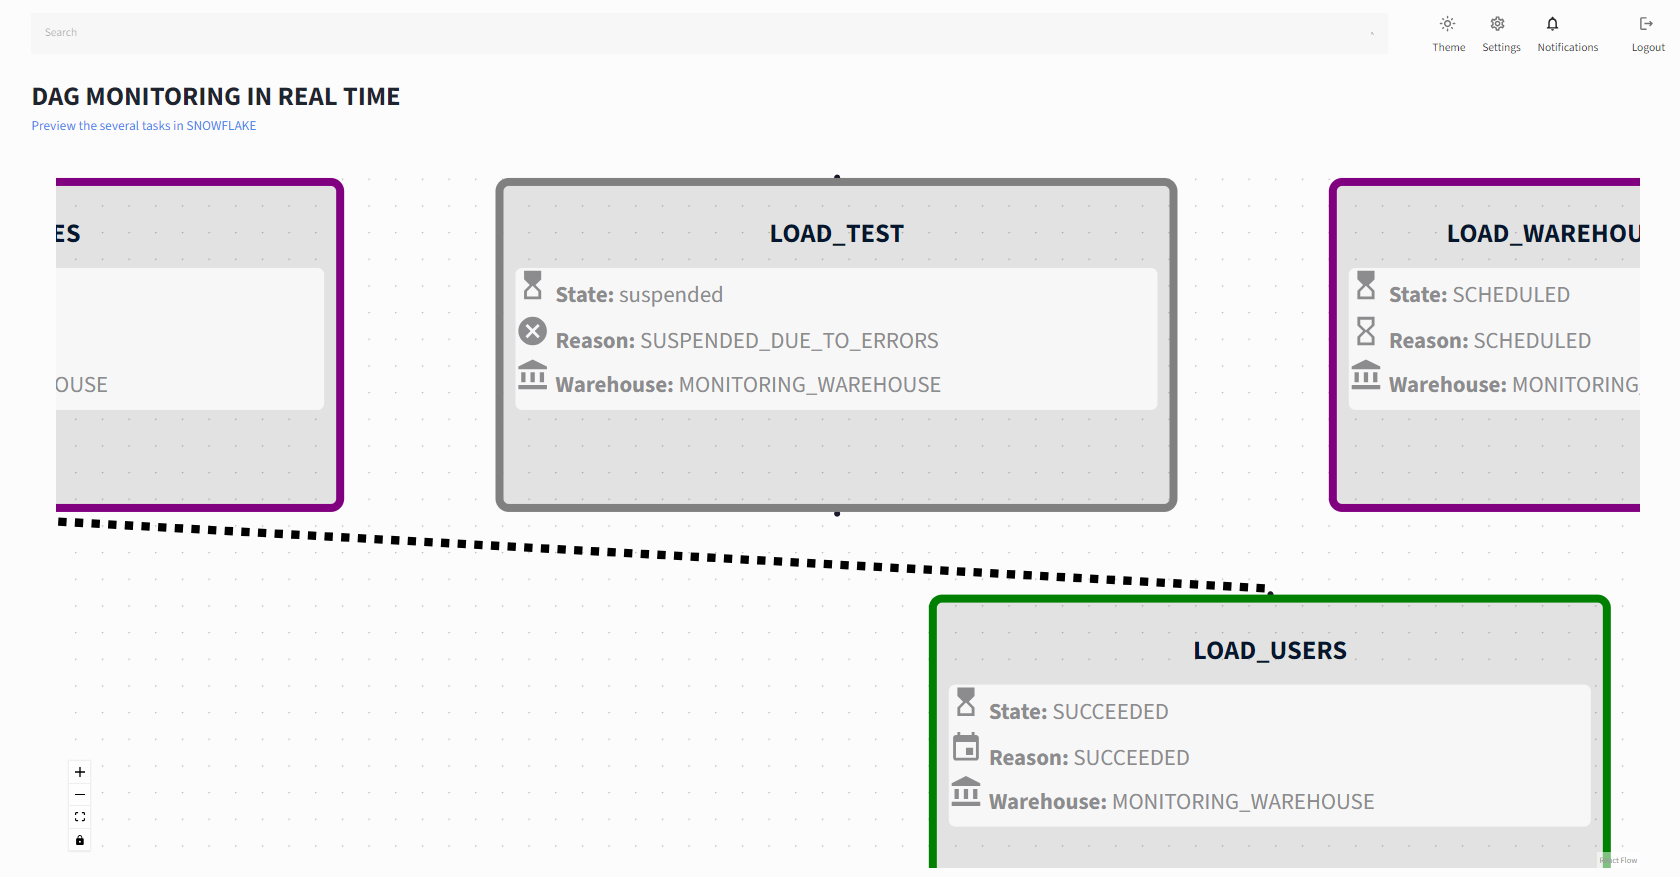
\includegraphics[width =1\linewidth]{img/captures/dag/final/error.png}
    \caption{Auto-suspend de la tâche}
    \label{fig:autosus}
    \end{figure}
\par Nous allons prendre l' exemple si la tâche <<Load schemas>> est erronée:  La figure \textbf{\ref{fig:dagerror}} illustre l'état du DAG à cet instant. 
\begin{figure}[H]
    \centering
    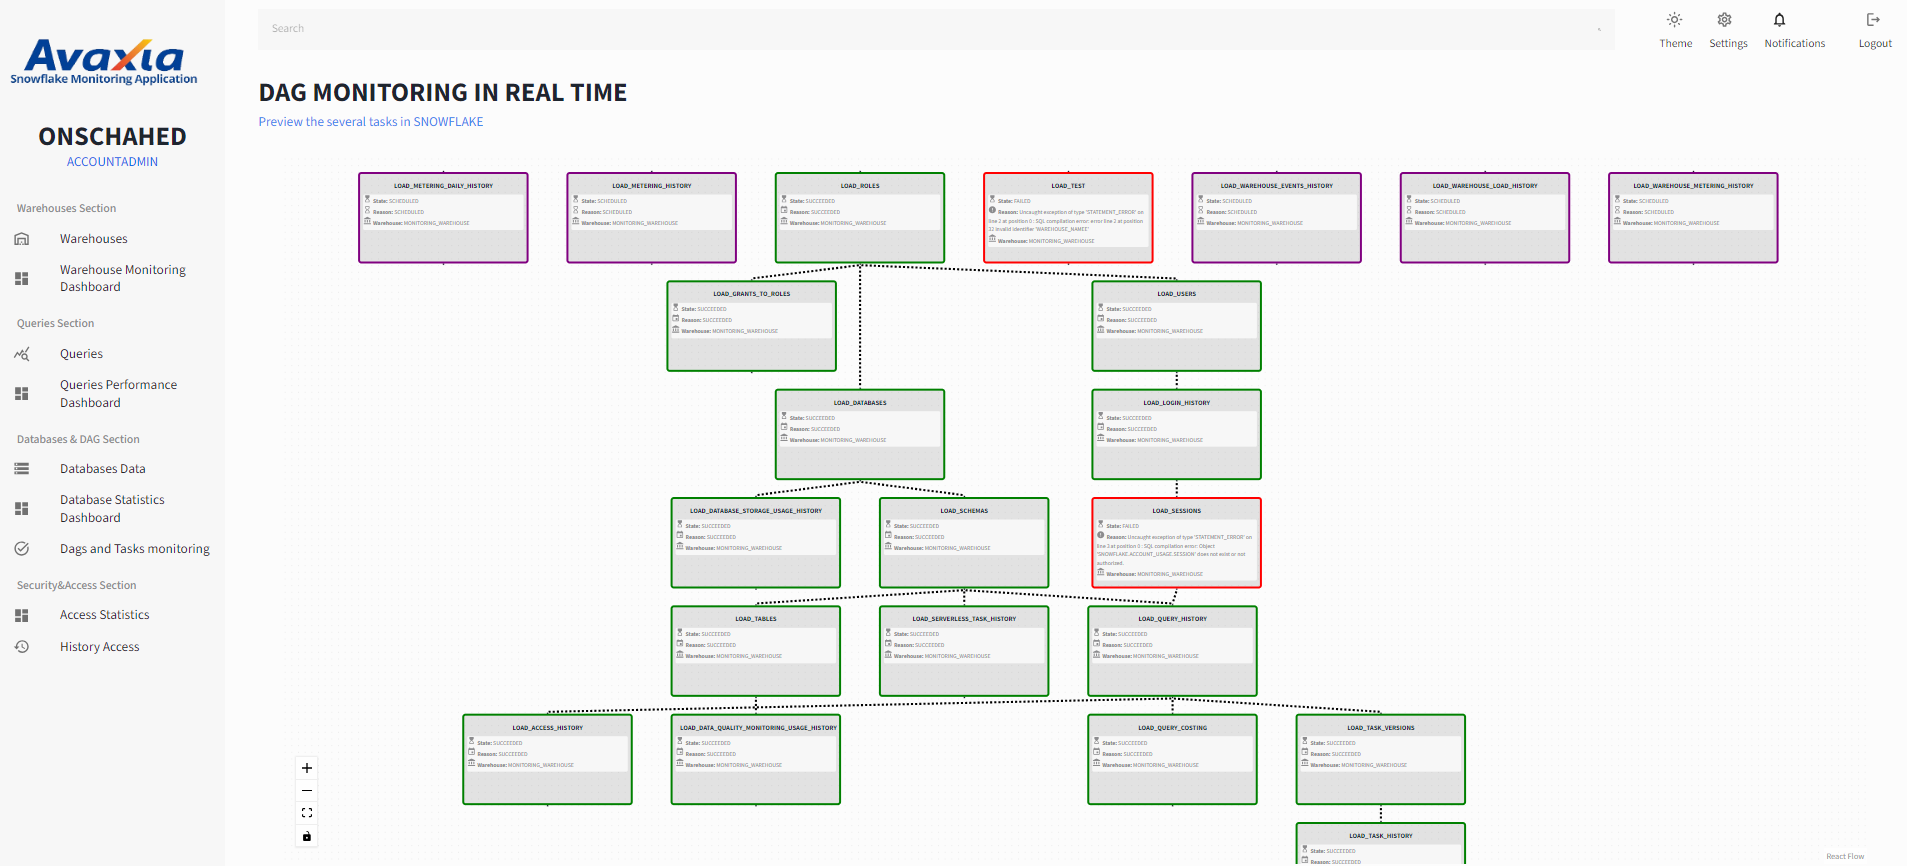
\includegraphics[width =1\linewidth]{img/captures/dag/final/schemaerror.png}
    \caption{DAG erronée}
    \label{fig:dagerror}
    \end{figure}
\par Aprés 10 tentatives, la racine du DAG est suspendu automatiquement à cause de cette tâche ce qui est illustré par les figures \textbf{\ref{fig:root}} et \textbf{\ref{fig:roles}}. De plus, les autres tâches vont conserver leurs derniers états comme l'indique la figure \textbf{\ref{fig:root}}
\begin{figure}[H]
    \centering
    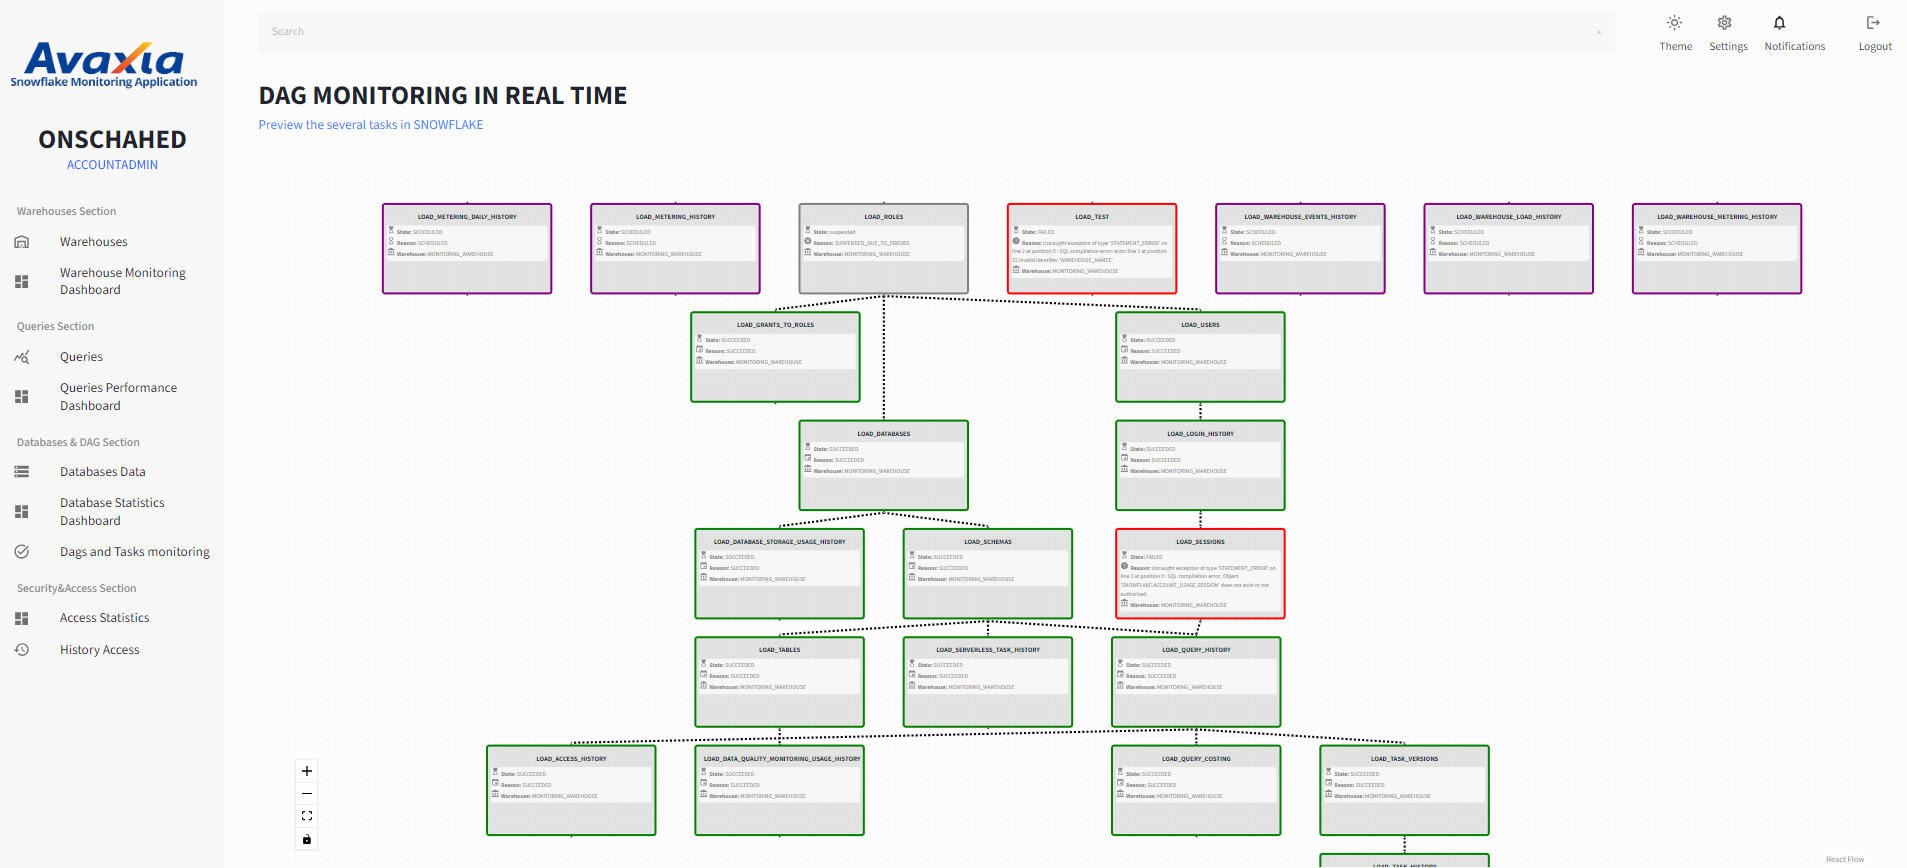
\includegraphics[width =1\linewidth]{img/captures/dag/final/auto_suspend_root.png}
    \caption{La racine de Dag est suspendu automatiquement}
    \label{fig:root}
\end{figure}
\begin{figure}[H]
    \centering
    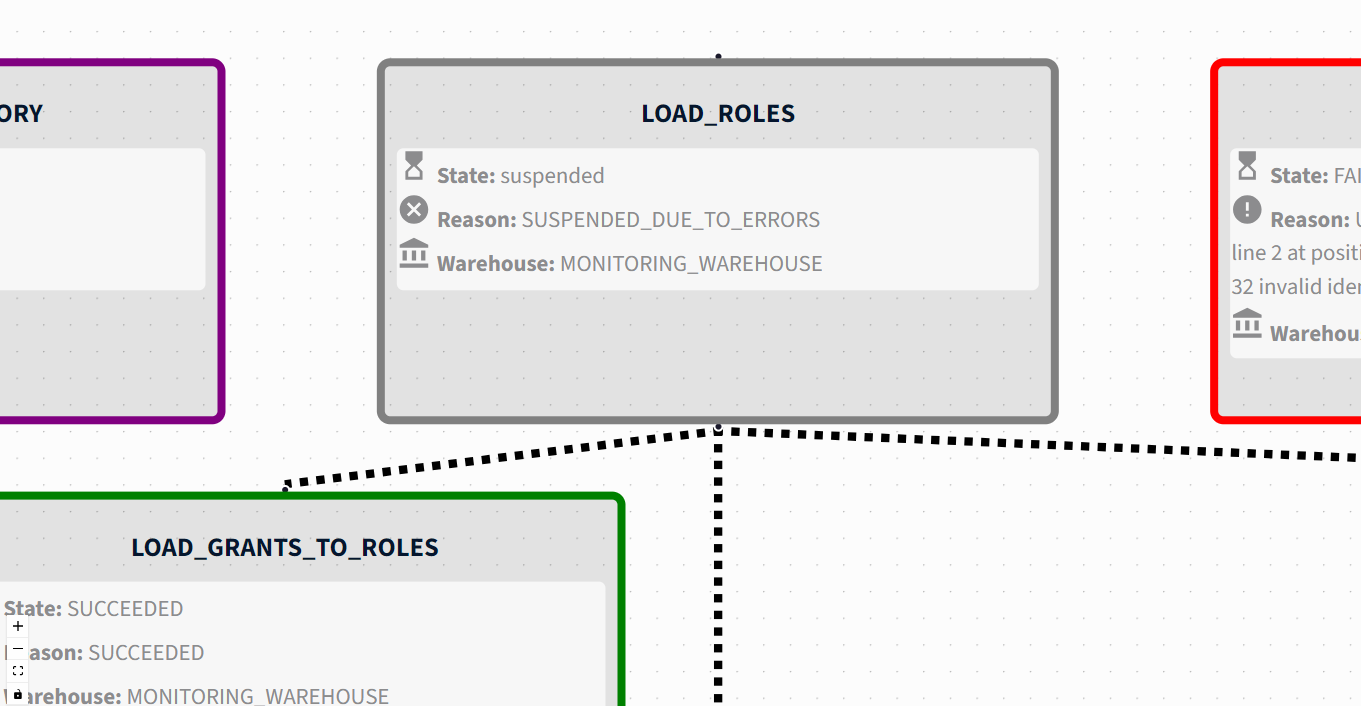
\includegraphics[width =1\linewidth]{img/captures/dag/final/roles.png}
    \caption{Détails de suspend de la racine}
    \label{fig:roles}
\end{figure}
\par En conclusion, ce microservice offre une vue d'ensemble détaillée et interconnectée du suivi des Tâches et des DAGs au sein du compte Snowflake.
Cette approche intégrée donne aux administrateurs une compréhension globale de l'environnement, facilitant la détection rapide des problèmes, le diagnostic des causes et la mise en place de mesures correctives pour assurer la fiabilité et l'efficacité des données qui circule dans les entrepôts de données ainsi que l'environnement Snowflake.
\subsection{Micro-service <<Notifications\_Launcher>>}
\par Ce micro-service est responsable de l'envoi des notifications aux utilisateurs concernés selon l'évenement qui peut apparaître.
\begin{itemize}
    \item \textbf{Si les mise à jours sont effectuées :}
        \par Dans le cas où les mise à jours sont effectuées pour un compte, et comme nous avons déjà préciser dans le  microservice d'authentification, une fois le process ETL termine sont exécution il lance une notification à MQTT Broker, la figure \textbf{\ref{fig:step1}} rillustre une autre fois cette partie: 
        \begin{figure}[H]
            \centering
            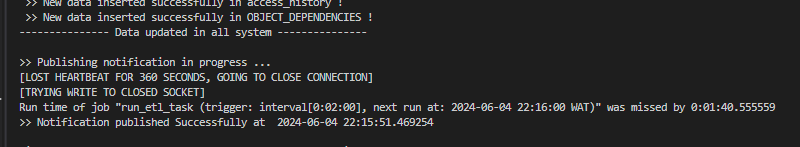
\includegraphics[width =1\linewidth]{img/captures/notifications/updatelaunch.png}
            \caption{Exécution de l'ETL}
            \label{fig:step1}
        \end{figure}
        \par la publication de cette nouvelle notification dans MQTT est illustrée par la figure \textbf{\ref{fig:step2}} suivante :
        \begin{figure}[H]
            \centering
            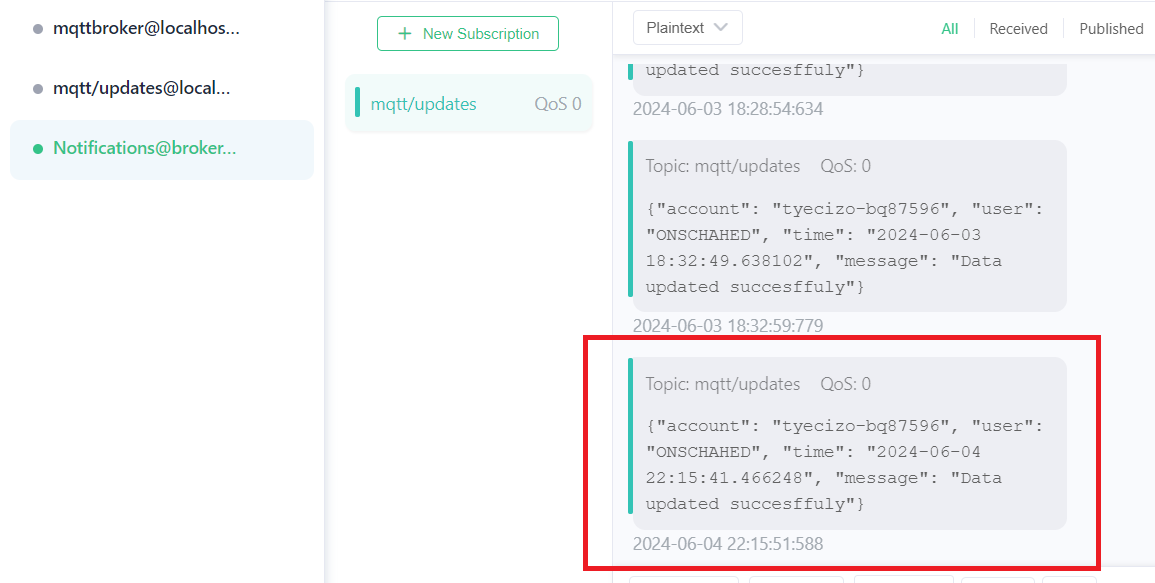
\includegraphics[width =1\linewidth]{img/captures/notifications/mqtt.png}
            \caption{Publication dans le topic <<Mqtt/updates>>}
            \label{fig:step2}
        \end{figure}
        \par Simultanément, dans notre application, une popup s'affiche pour notifier les utilisateurs connectés à ce compte qu'un mise à jour a était effectuée.
        La figure \textbf{\ref{fig:step3}} illustre la récéption de la nouvelle notification : 
        \begin{figure}[H]
            \centering
            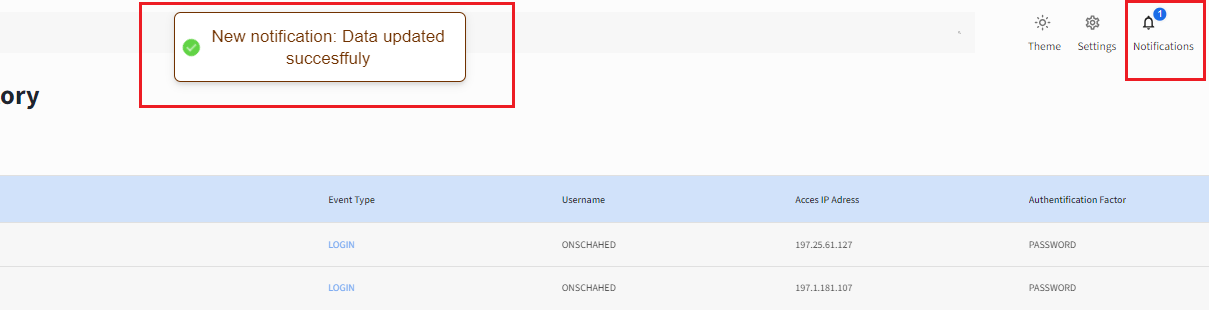
\includegraphics[width =1\linewidth]{img/captures/notifications/new_update.png}
            \caption{Réception de la nouvelle notification de mise à jour dans <<Snowflake Monitoring Application>>}
            \label{fig:step3}
        \end{figure}
        \par une fois nous cliquons sur l'icône de notification, la liste des notifications pour cet utilisateur s'affiche, comme l'indique la figure \textbf{\ref{fig:step4}} : 
        \begin{figure}[H]
            \centering
            \begin{tabular}[b]{c}
            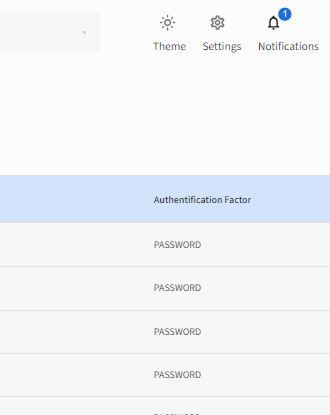
\includegraphics[width=0.3\linewidth ,height=7cm]{img/captures/notifications/notif.png} \\
            
            \end{tabular} 
            \begin{tabular}[b]{c}
            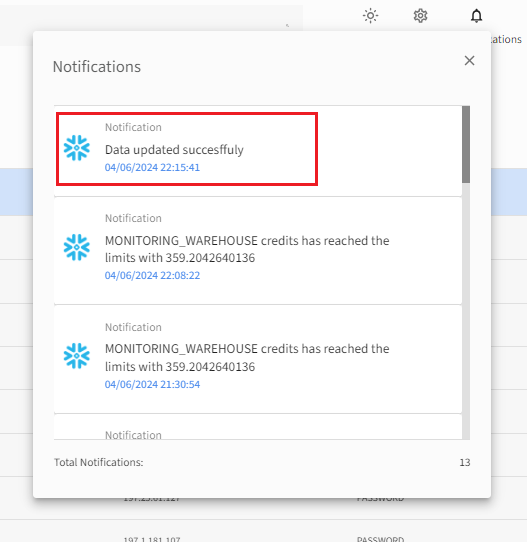
\includegraphics[width=0.3\linewidth ,height=7cm]{img/captures/notifications/update2.png} \\
            
            \end{tabular}
            \caption{Consultation des notifications}
        \label{fig:step4}
        \end{figure}

    \item \textbf{Si les limites de consommation sont atteintes :}
    \par Dans le cas où les limites de consommation sont atteintes pour un des entrepôt de données, une notification est lancée. 
    \par Nous prenons l'exemple de modification de limites à 50\$ dans les paramétres globaux et nous allons surveiller ce que va se passer dans notre application. 
    \par La figure \textbf{\ref{fig:global1}} illustre la modification des paramétres pour surveiller le lancement des notifications:
    \begin{figure}[H]
        \centering
        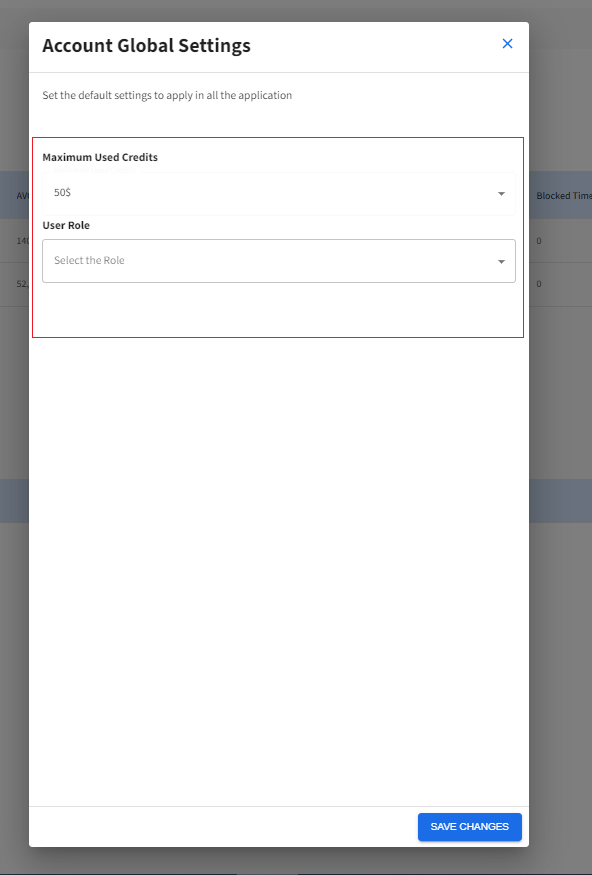
\includegraphics[width=0.3\linewidth ,height=8cm]{img/captures/notifications/settings.png}
        \caption{Modification de limites}
        \label{fig:global1}
    \end{figure}
    \par Une fois la modification est effectuée, nous allons simuler une publication dans le topic <<mqtt/credits>> comme l'indique la figure \textbf{\ref{fig:global2}}. 
    \\ Cette fois ci, la publication dans MQTT est faite par le frontend de ce microservice.
    \begin{figure}[H]
        \centering
        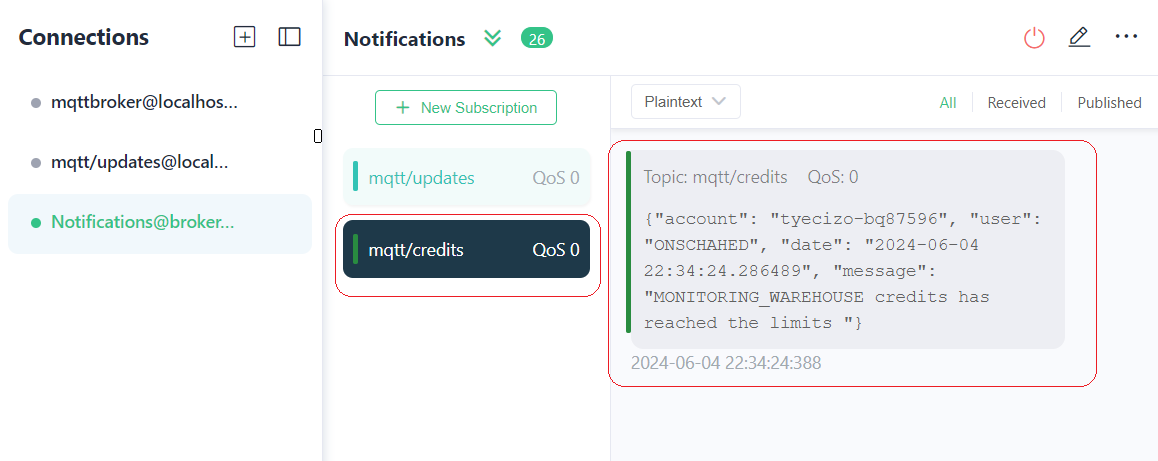
\includegraphics[width =1\linewidth]{img/captures/notifications/mqtt_global.png}
        \caption{Publication dans le topic <<Mqtt/credits>>}
        \label{fig:global2}
    \end{figure}
    \par Parallélement, Une notification est reçue dans l'application et une popup s'affiche pour indiquer la reception de cette dernière. La figure \textbf{\ref{fig:global3}} illustre la récéption de la notification :
    \begin{figure}[H]
        \centering
        \includegraphics[width =1\linewidth]{img/captures/notifications/newglobal.png}
        \caption{Récéption de la nouvelle notification}
        \label{fig:global3}
    \end{figure}
    \par Une fois nous cliquons sur l'icône de notification, la liste s'affiche avec la nouvelle notification.
    \par La figure \textbf{\ref{fig:global4}} représente la nouvelle liste des notifications :
    \begin{figure}[H]
        \centering
        \begin{tabular}[b]{c}
        \includegraphics[width=0.3\linewidth ,height=7cm]{img/captures/notifications/newLimit.png} \\
        
        \end{tabular} 
        \begin{tabular}[b]{c}
        \includegraphics[width=0.3\linewidth ,height=7cm]{img/captures/notifications/notifglobal.png} \\
        
        \end{tabular}
        \caption{Consultation des notifications}
    \label{fig:global4}
    \end{figure}
\end{itemize}
\par En conclusion, ce microservice joue un rôle essentiel dans la chaîne de valeur de l'application. En agissant comme une passerelle entre le service ETL et les utilisateurs finaux, il garantit que les informations 
critiques sont rapidement et efficacement communiquées.  
\subsection{Personnalisation de l'interface utilisateur : thèmes clair et sombre}
\par Dans ce projet, nous avons intégré des fonctionnalités de personnalisation pour améliorer l'expérience utilisateur, notamment le développement de thèmes clair et sombre. \\ Cette double option permet aux 
utilisateurs de choisir entre une interface lumineuse et une interface sombre, en fonction de leurs préférences ou des conditions de luminosité ambiante. Le thème clair offre une visualisation nette et claire idéale
 pour les environnements bien éclairés, tandis que le thème sombre réduit la fatigue oculaire lors d'une utilisation prolongée dans des conditions de faible luminosité. Cette flexibilité assure une meilleure ergonomie 
 et accessibilité de notre application, répondant ainsi aux attentes variées de notre base d'utilisateurs diversifiée.
 La figure \textbf{\ref{fig:theme}} illustre l'option <<theme>> qui nous permet de modifier le théme :
 \begin{figure}[H]
    \centering
    \begin{tabular}[b]{c}
        \includegraphics[width=0.3\linewidth,height=3cm ]{img/captures/dark/5.jpg}
        \end{tabular}
        \begin{tabular}[b]{c}
            \includegraphics[width=0.3\linewidth ,height=3cm]{img/captures/dark/7.jpg}
            \end{tabular}
            \caption{Modification du théme}
            \label{fig:theme}
\end{figure}
\newpage
\par La figure \textbf{\ref{fig:dark1}} suivante illustrent les interfaces de <<Databases Dashboard >> et <<Database Objects List >> en mode sombre :
 \begin{figure}[H]
    \centering
    \begin{tabular}[b]{c}
        \includegraphics[width=1\linewidth,height= 10cm]{img/captures/dark/2.jpg}
        \end{tabular}
        \begin{tabular}[b]{c}
            \includegraphics[width=1\linewidth ,height= 10cm]{img/captures/dark/4.jpg}
            \end{tabular}
            \caption{Interfaces <<Databases Dashboard >> et <<Database Objects List >> en thème sombre}
            \label{fig:dark1}
\end{figure}
\newpage
\par La figure \textbf{\ref{fig:dark2}} suivante illustrent les interfaces de <<Queries Dashboard >> et <<Warehouses List >> en mode sombre :
 \begin{figure}[H]
    \centering
    \begin{tabular}[b]{c}
        \includegraphics[width=1\linewidth ,height=7cm]{img/captures/dark/1.jpg}
        \end{tabular}
        \begin{tabular}[b]{c}
            \includegraphics[width=1\linewidth,height=7cm]{img/captures/dark/3.jpg}
            \end{tabular}
            \caption{Interfaces en <<Queries Dashboard >> et <<Warehouses List >> thème sombre}
            \label{fig:dark2}
\end{figure}


\section*{Conclusion}
\addcontentsline{toc}{section}{Conclusion }
Ce chapitre résume le travail accompli pour donner forme à notre projet. Les choix techniques que nous avons adoptés et 
détaillés nous ont permis de concrétiser notre vision. De plus, nous avons pu présenter la réalisation de ce projet en
 illustrant chaque partie avec des captures explicatives, montrant ainsi le cheminement de notre démarche. 
\\Dans la conclusion générale, nous réunisserons l'ensemble de notre travail et soulignerons les perspectives pour l'avenir. 